\chapter{Resultados}
\label{sec:resultados}

Este capítulo organiza la evidencia por dispositivo. Primero se presentan los resultados de la campaña final de CPU. Después se reportan la validación del instrumento GPU, el diagnóstico exploratorio de su primer conjunto de entrenamiento y el cambio posterior de la estrategia de medición. Esta distinción evita presentar resultados intermedios como conclusiones finales. Las tablas y figuras de sensibilidad, desglose y trazabilidad se conservan en el Anexo \ref{anexo:resultados-complementarios}; el cuerpo principal mantiene la evidencia necesaria para seguir cada conclusión.

\section{Resultados de CPU}
\label{sec:resultados-cpu}

El conjunto de CPU procede de una campaña que cubrió 49 configuraciones de kernel en el nivel nativo y nueve niveles fijos de frecuencia, con tres repeticiones por combinación, y sus 1470 corridas finalizaron aceptadas. En esta campaña, el warmup se calibró a partir de las ventanas medidas para cada kernel y el conjunto se reprocesó con esos valores; los transitorios fueron pequeños, con un máximo de 4.8\% de la duración de corrida y valores inferiores a 2\% en la mayoría de los kernels.

La unidad que alimenta el conjunto de entrenamiento CPU es el intervalo real de \textit{uncore} de aproximadamente 10~ms (sección \ref{sec:granularidad}). La Tabla \ref{tab:cpu-cobertura-conjunto} resume la cobertura obtenida después del filtrado de calidad. De 1\,424\,531 intervalos procesados, 1\,309\,755 cumplieron simultáneamente los criterios de telemetría y de frecuencia. Los restantes se conservaron para auditoría, pero no recibieron una etiqueta de entrenamiento.

\subsection{Composición de fase por kernel}
\label{sec:resultados-cpu-composicion}

Las cargas y su suite de origen se enumeran en la Tabla \ref{tab:catalogo}. La Figura \ref{fig:cpu-composicion-clase-kernel} muestra que el conjunto cubre ambos regímenes y conserva configuraciones próximas al \textit{ridge}.

\begin{figure}[H]
    \centering
    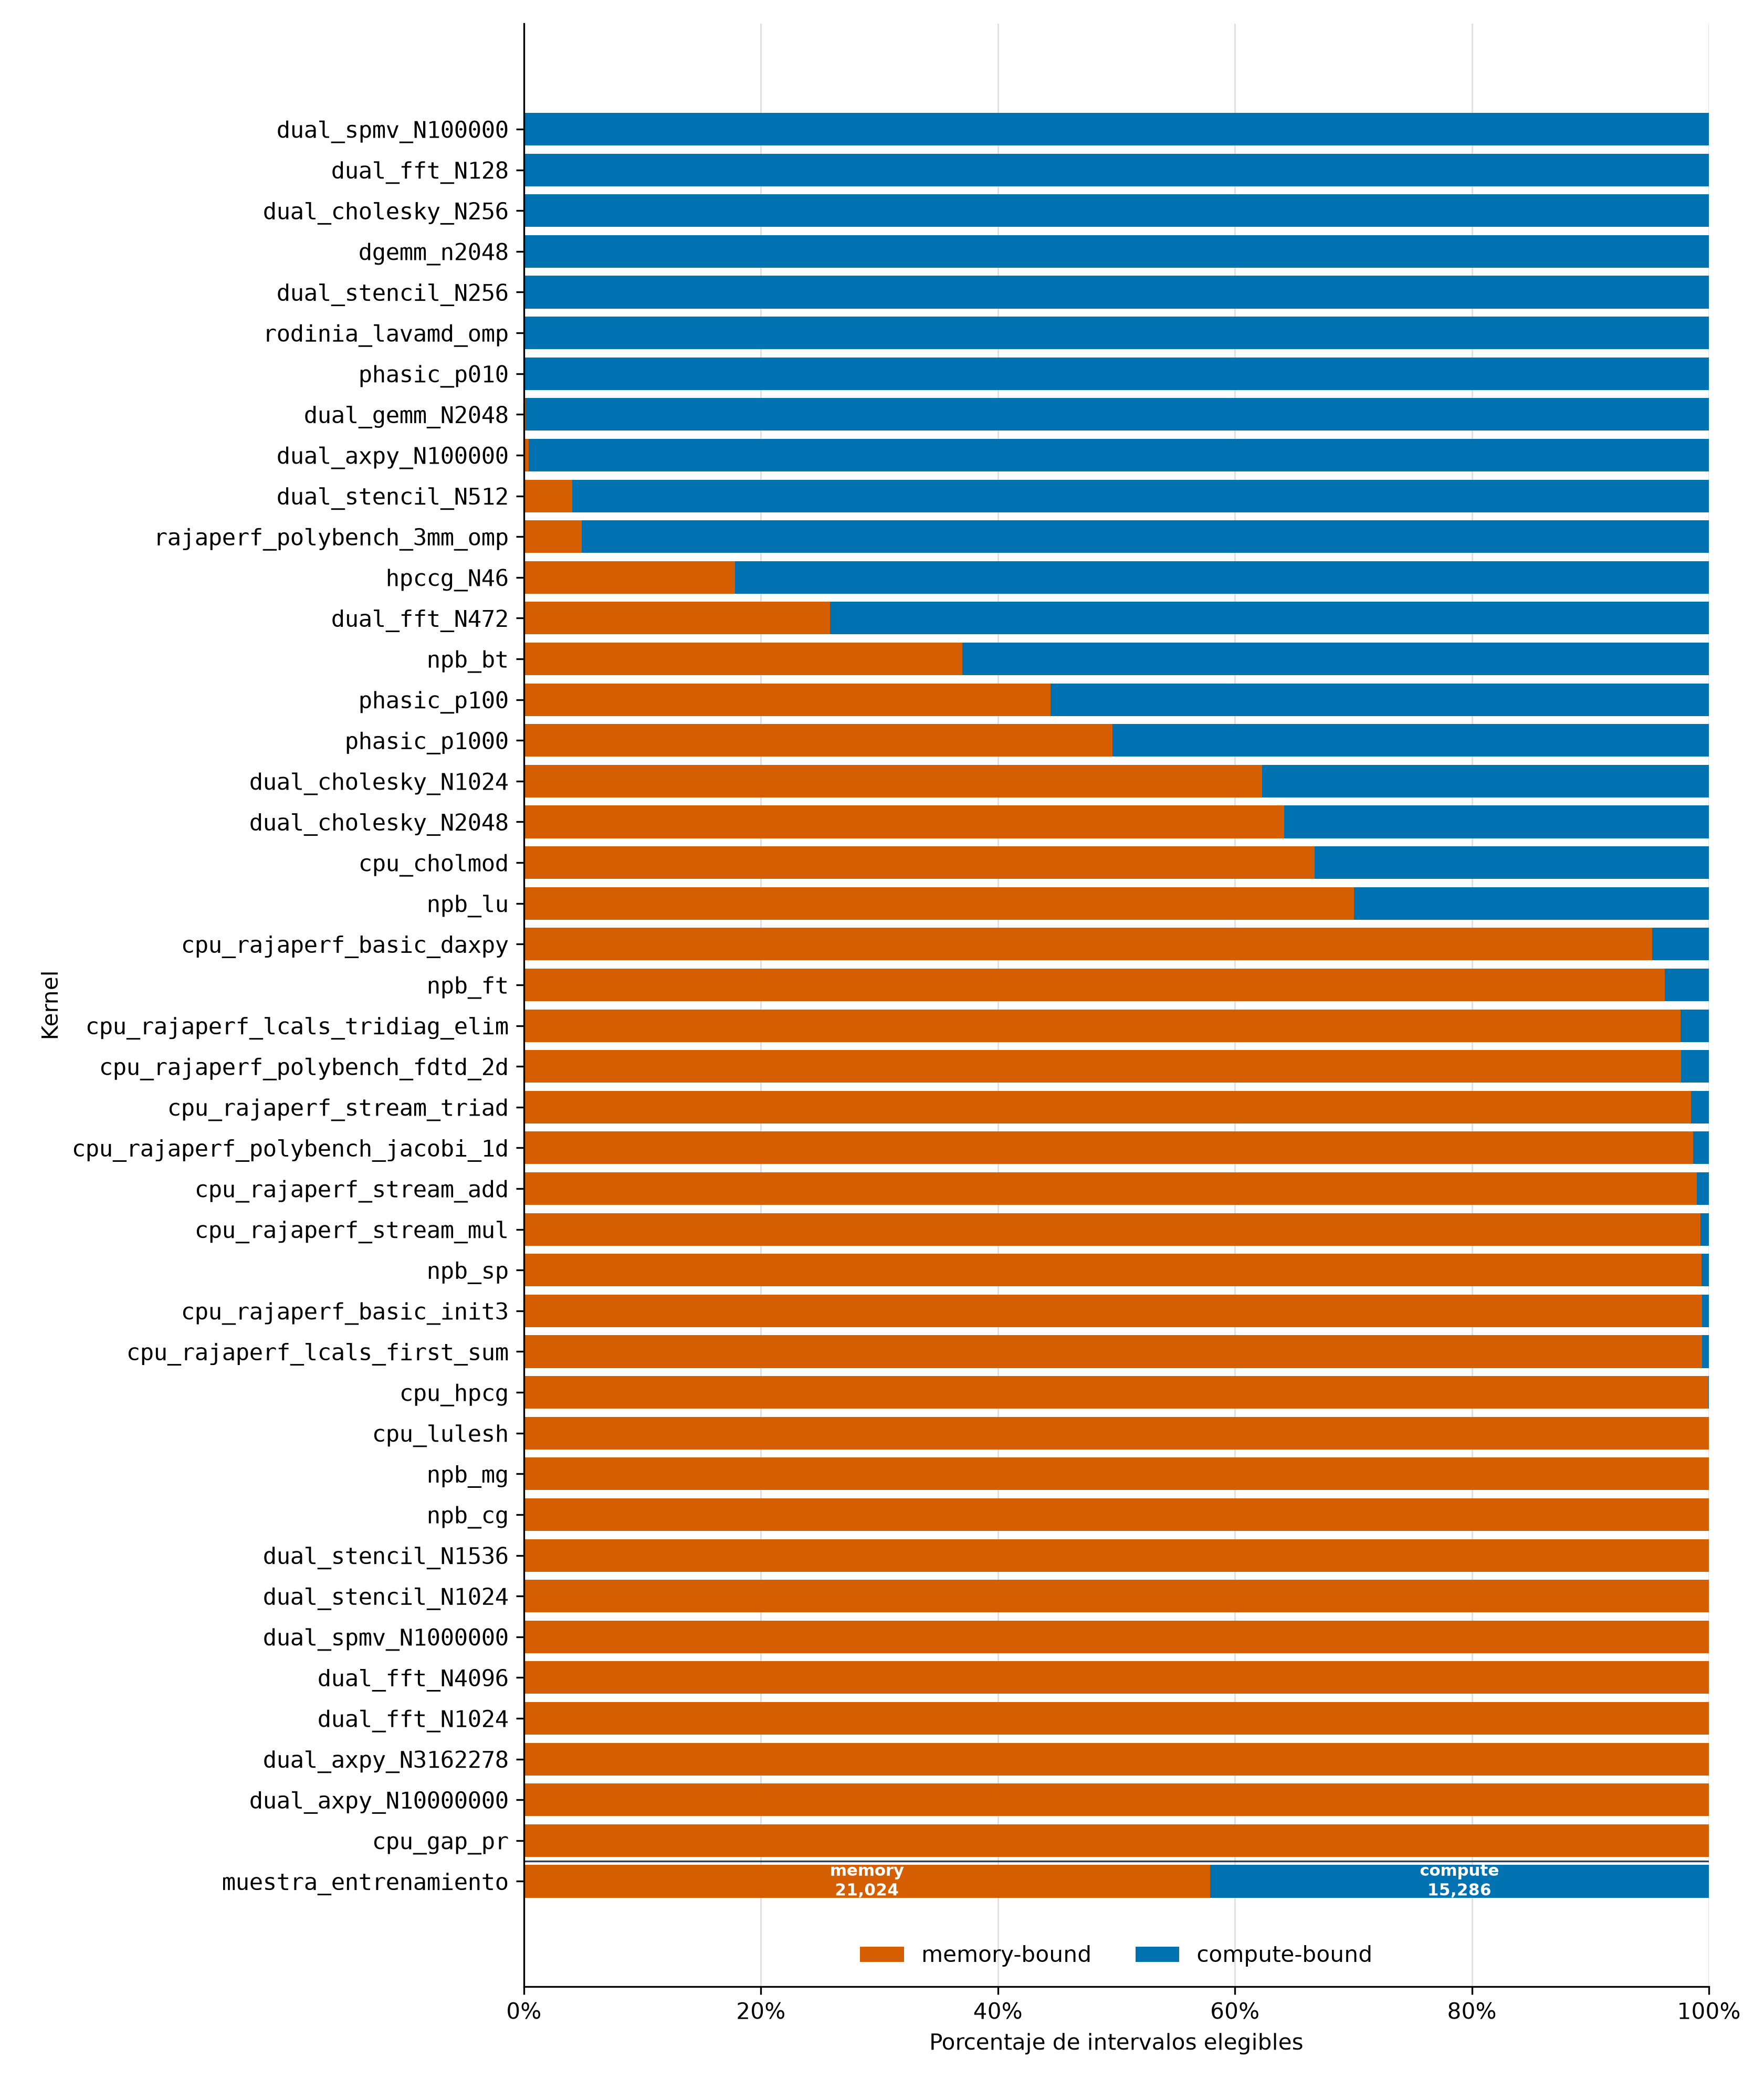
\includegraphics[width=0.60\textheight]
        {figuras/fig_cpu_composicion_clase_por_kernel_20260917.png}
    \caption[Composición de fase por kernel en CPU]{Porcentaje de intervalos elegibles clasificados \textit{compute\_bound} y \textit{memory\_bound} para cada configuración de kernel de la campaña CPU. La barra final resume la muestra usada por el clasificador, con 21\,350 intervalos \textit{compute\_bound} y 21\,108 intervalos \textit{memory\_bound}. Fuente: elaboración propia.}
    \label{fig:cpu-composicion-clase-kernel}
\end{figure}

La composición intermedia no se concentra en un solo algoritmo. \textit{npb\_bt}, \textit{npb\_lu}, \textit{cpu\_cholmod}, \textit{hpccg\_cpu\_N46}, las variantes \textit{phasic} y los tamaños dirigidos de FFT y Cholesky aportan intervalos de ambos regímenes. Estas configuraciones evitan que el conjunto quede limitado a ejemplos alejados del punto de inflexión.

Tres kernels de patrón de acceso irregular de Rodinia (\textit{kmeans}, \textit{srad} y \textit{particlefilter}) se midieron por separado y resultaron casi puramente \textit{memory-bound}; como no aportaban ejemplos \textit{compute-bound} ni mixtos, quedaron fuera del conjunto de entrenamiento por no añadir más que redundancia \textit{memory-bound}.


\subsection{Variación de la composición con la frecuencia}
\label{sec:resultados-cpu-frecuencia}

La proporción global de intervalos \textit{compute\_bound} aumentó desde 29.0\% en el nivel nativo hasta 46.4\% en F8, el nivel fijo más bajo. La Figura \ref{fig:cpu-composicion-clase-frecuencia} presenta esta variación. El resultado es consistente con un \textit{ridge} que disminuye cuando baja el techo de cómputo, de modo que una parte de los intervalos cercanos a la frontera cambia de etiqueta. La figura agrega todas las configuraciones y debe leerse junto con la composición por kernel, porque las cargas no aportan el mismo número de intervalos.

\begin{figure}[H]
    \centering
    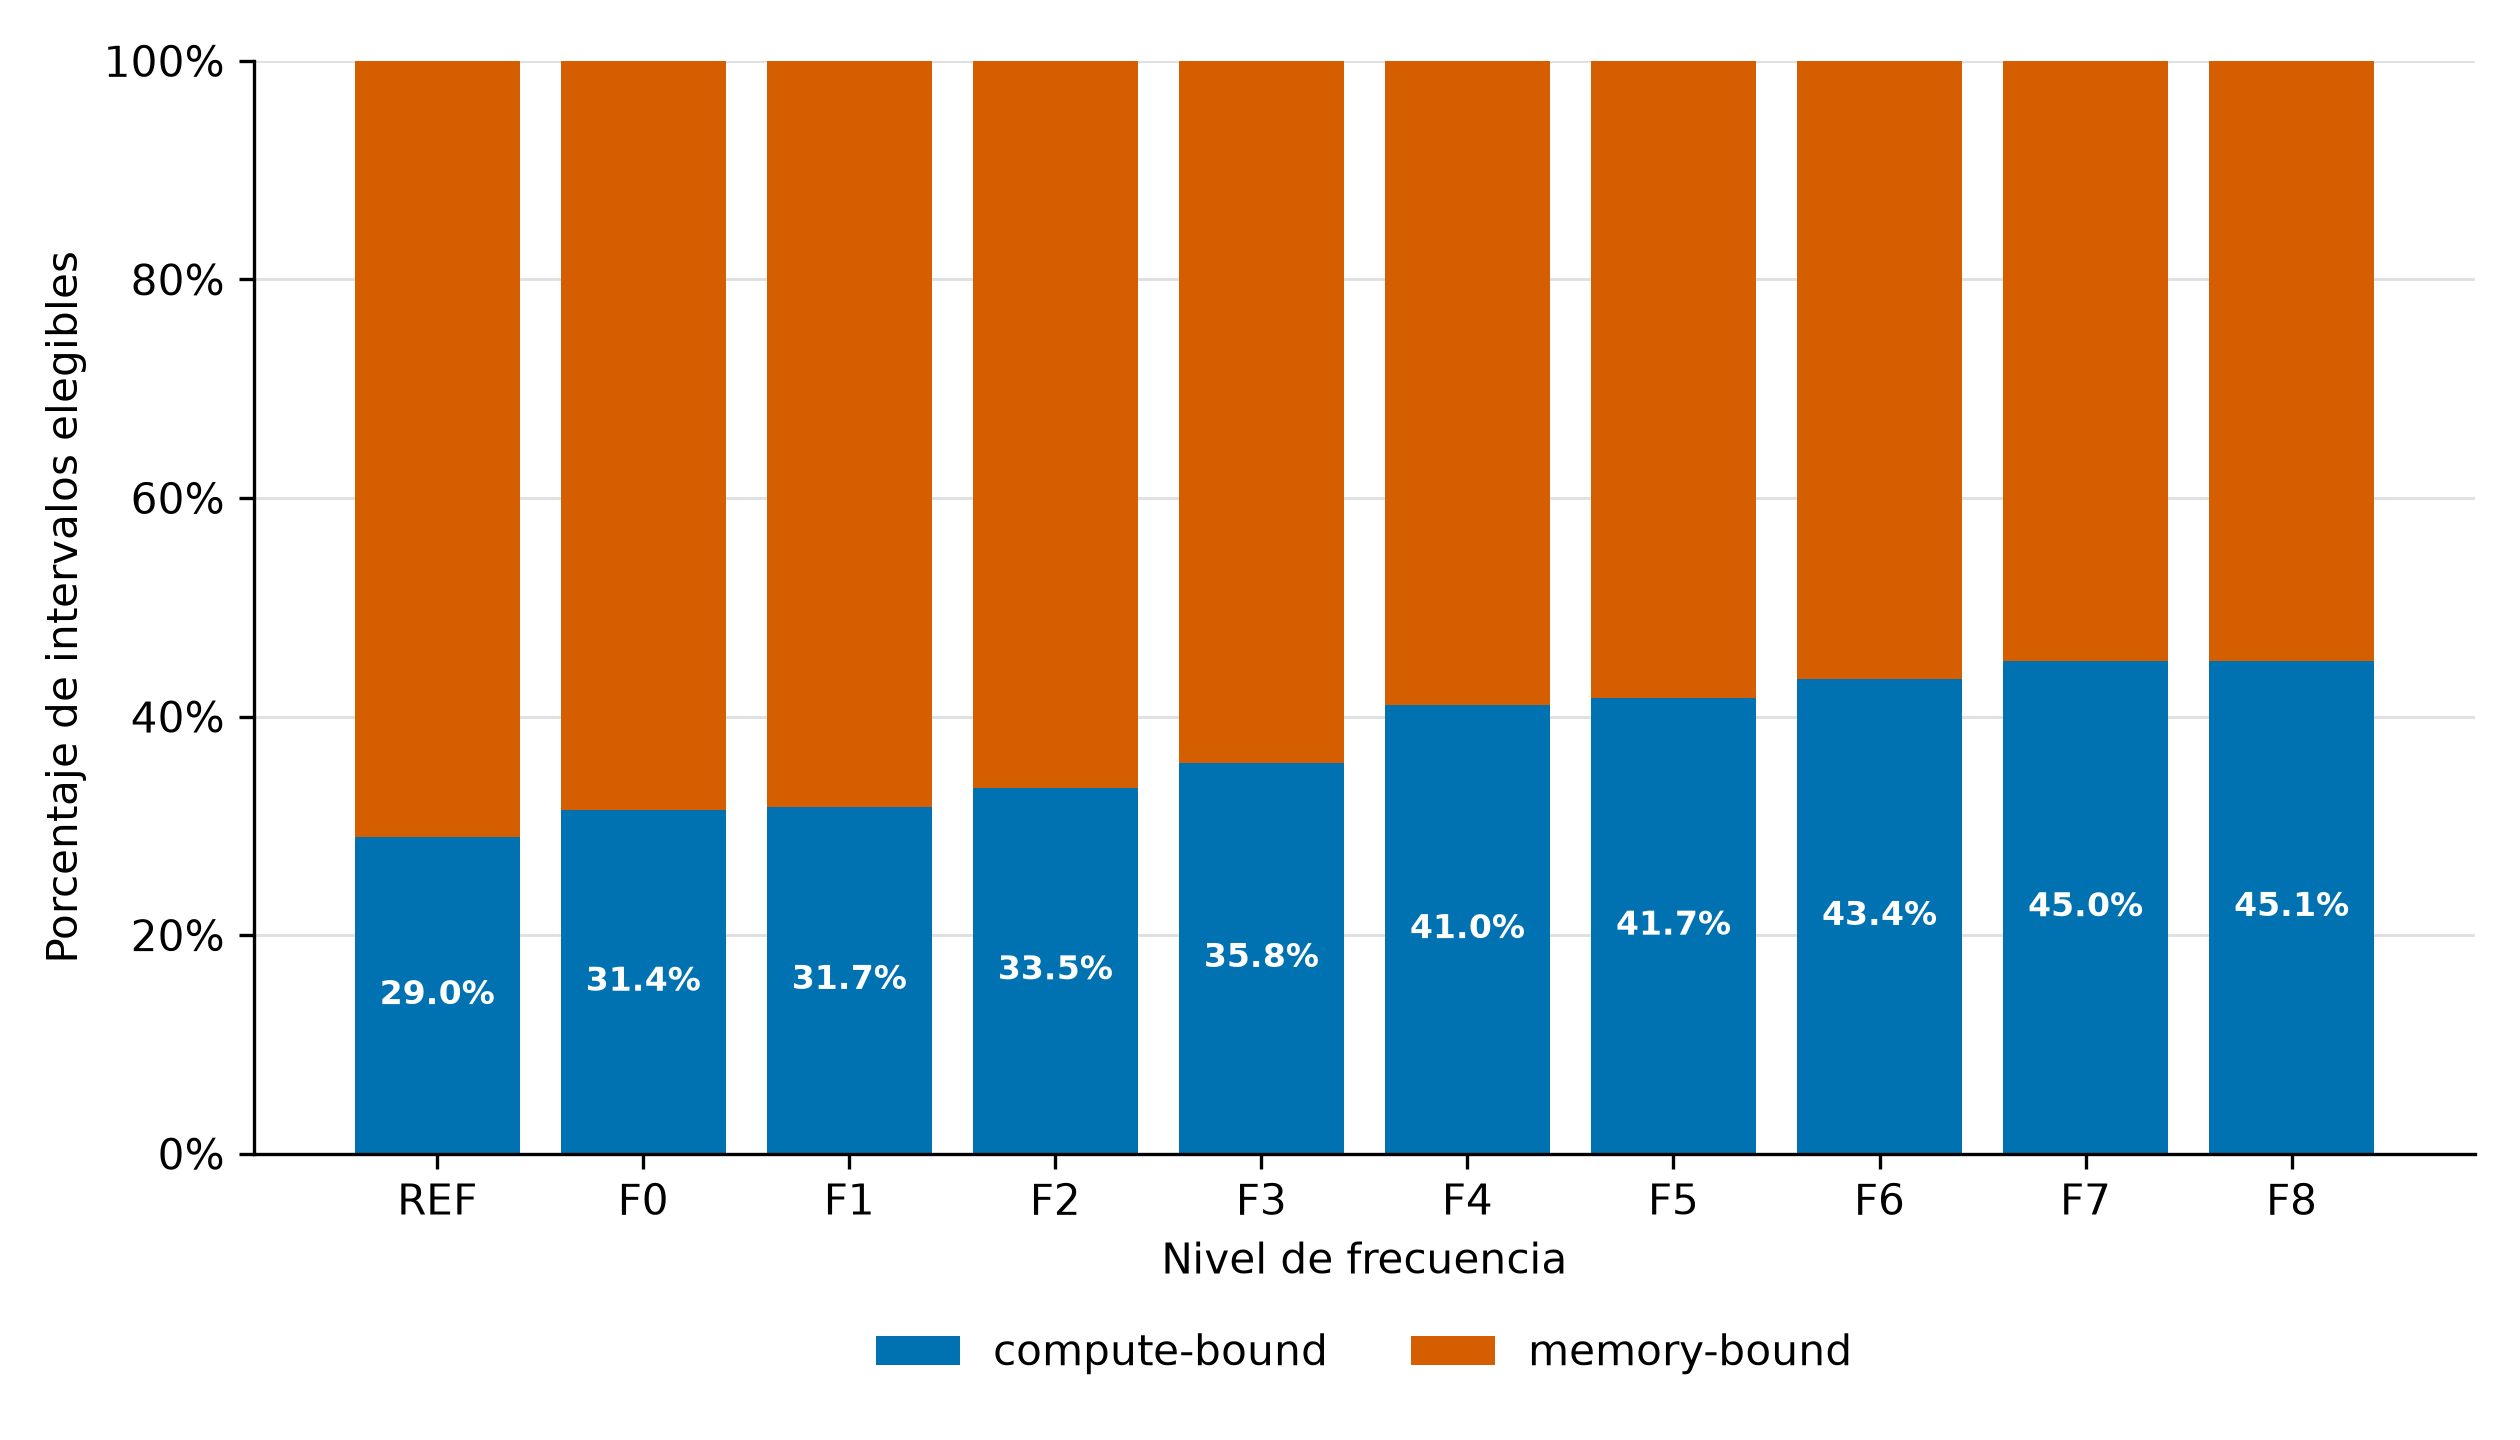
\includegraphics[width=0.9\textwidth]
        {figuras/fig_cpu_composicion_clase_por_frecuencia_20260917.png}
    \caption[Composición de fase por nivel de frecuencia en CPU]{Porcentaje de intervalos elegibles clasificados \textit{compute\_bound} y \textit{memory\_bound} en cada nivel de frecuencia de la campaña CPU. Fuente: elaboración propia.}
    \label{fig:cpu-composicion-clase-frecuencia}
\end{figure}


\subsection{Calidad del conjunto de datos}
\label{sec:resultados-cpu-dvfs}

Las 1470 corridas CPU se aceptaron con turbo desactivado y verificación del reloj observado dentro de $\pm5\%$. Se descartaron los márgenes de transición (unos 10~ms) y de inicio y final (0.15~s), además de las ventanas con frecuencia o telemetría no utilizable. En total, el 91.9\% de los 1\,424\,531 intervalos procesados quedó elegible (Tabla \ref{tab:cpu-rechazos}). La prueba de actuación confirmó que era necesario restringir también los hilos hermanos de \textit{SMT}.

\paragraph{Medición de bytes y etiqueta.}\label{sec:resultados-uncore}
Los bytes movidos en memoria se leen de los contadores de \textit{uncore} del controlador de memoria (sección \ref{sec:uncore}), y son la única fuente de bytes de la etiqueta. La etiqueta de cada intervalo compara los FLOPs medidos con esos bytes contra el \textit{ridge} calibrado para su nivel de frecuencia. La Figura \ref{fig:ridge-frecuencia} presenta cómo desciende el \textit{ridge} conforme baja la frecuencia. El presupuesto simultáneo es de nueve eventos de PMU y no diez, porque el vigilante NMI del sistema operativo reserva un contador físico por núcleo. Los contadores de \textit{uncore} son de alcance de sistema, por lo que cada campaña exige el nodo en exclusiva; con esa condición, la cadencia de intervalos se sostuvo en los $\sim$10~ms esperados a lo largo de toda una corrida de prueba. Antes de la campaña completa se ejecutaron dos campañas de humo a escala reducida (18 y 21 combinaciones) que ejercitaron el mismo camino de código y se aceptaron por completo; con clasificaciones coherentes: la multiplicación densa de matrices fue \textit{compute-bound} en el 100\% de sus ventanas y los kernels de NAS resultaron predominantemente \textit{memory-bound}.\label{sec:resultados-interferencia-uncore}

\begin{figure}[H]
\centering
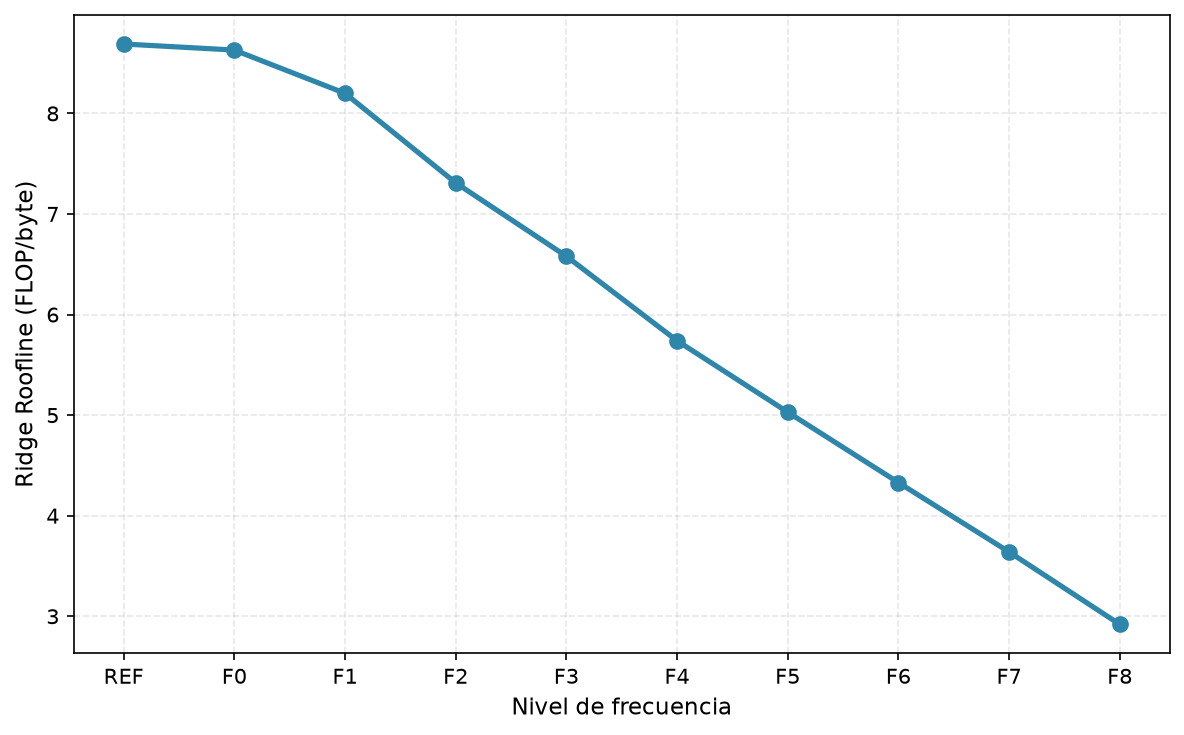
\includegraphics[width=0.6\textwidth]{figuras/fig_ridge_por_frecuencia_20260920.png}
\caption{\textit{Ridge} Roofline según el nivel de frecuencia CPU. El punto de inflexión desciende de 8.69~FLOP/byte en referencia nativa a 2.92~FLOP/byte en F8. Fuente: elaboración propia.}
\label{fig:ridge-frecuencia}
\end{figure}

La Figura \ref{fig:cpu-roofline-scatter} sitúa los intervalos del conjunto de entrenamiento directamente en el plano Roofline, contra el techo calibrado de cada nivel. Los FLOPs y bytes por intervalo no forman parte del vector de entrada del clasificador (sección \ref{sec:contrato-features}), por lo que esta vista se reconstruye aparte, sobre las mismas corridas de la campaña, y se muestra solo para REF y F8 como los extremos del rango de frecuencia. La nube \textit{memory-bound} queda, en su mayoría, bajo la rampa de ancho de banda a la izquierda del \textit{ridge}, y la nube \textit{compute-bound} bajo el techo plano de cómputo a la derecha; ambas quedan muy por debajo del techo teórico, porque los kernels reales sostienen una fracción de la tasa aritmética pico que un microbenchmark de registro alcanza (sección \ref{sec:roofline}). La franja de intervalos que cruza el \textit{ridge} en ambos sentidos es la misma ambigüedad que cuantifica la Figura \ref{fig:cpu-margen-ridge}.

\begin{figure}[H]
\centering
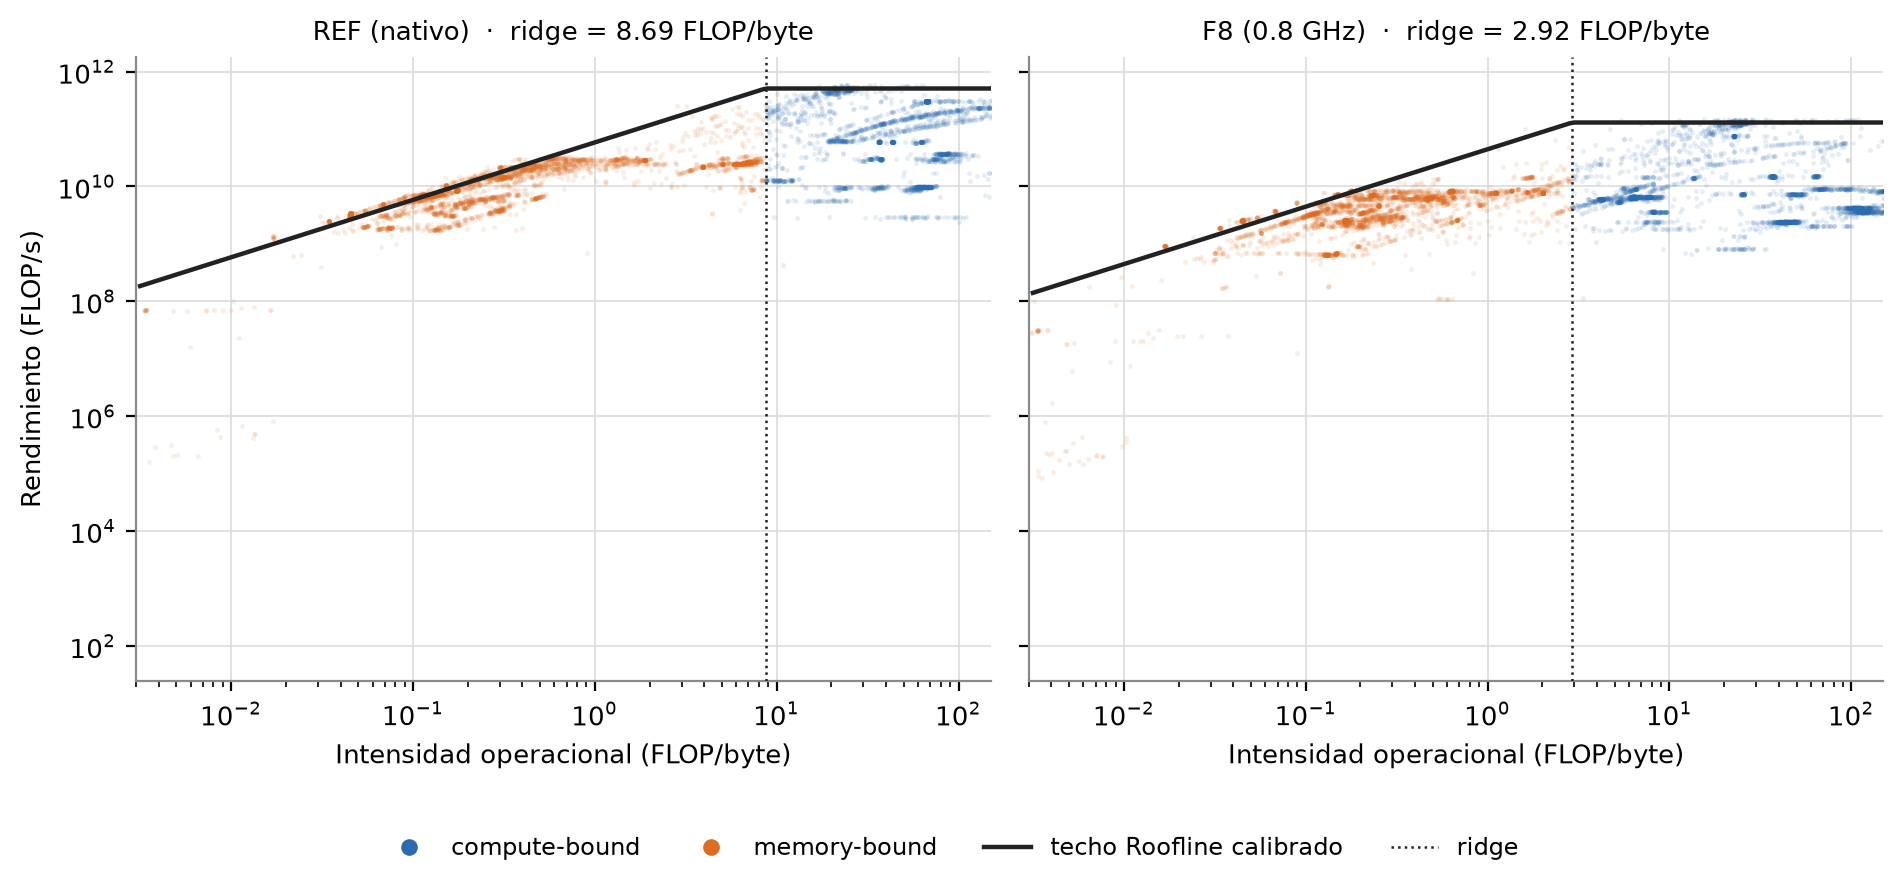
\includegraphics[width=0.98\textwidth]{figuras/fig_cpu_roofline_scatter_20260922.png}
\caption[Intervalos del conjunto de entrenamiento en el plano Roofline]{Submuestreo estratificado (4000 por nivel y clase, semilla 20260918) de los intervalos elegibles de REF y F8 en el plano intensidad--rendimiento, con el techo Roofline calibrado de cada nivel. Fuente: elaboración propia, reconstruido desde \path{training_cpu_intervals.csv} de la campaña \texttt{pacca\_cpu\_final\_20260913}.}
\label{fig:cpu-roofline-scatter}
\end{figure}

\paragraph{Validación de los techos Roofline.}\label{sec:resultados-ppico}
Los techos del modelo Roofline se calibraron de forma empírica sobre la propia plataforma (sección \ref{sec:roofline}). Para verificar esa calibración con un mecanismo independiente se empleó Intel Advisor, que contabiliza FLOPs y bytes mediante instrumentación binaria y no mediante contadores de PMU \cite{Advisor2026}. El ancho de banda calibrado coincide con el de Advisor dentro de 12 a 15\% (58.4 a 58.8~GB/s frente a 64.0 a 66.8~GB/s) y el techo de cómputo (417.8 a 555~GFLOP/s) es consistente con la referencia de Advisor, que midió 577.7~GFLOP/s sobre los mismos seis núcleos. El punto de inflexión del nivel nativo queda entre 7.0 y 9.3~FLOP/byte, compatible con los 8.69~FLOP/byte usados en la campaña, y desciende con el reloj hasta 2.92~FLOP/byte en F8, porque baja el techo de cómputo mientras el ancho de banda sigue limitado por memoria.


\subsection{Clasificador de fase en CPU}
\label{sec:resultados-cpu-clasificador}

Esta sección sigue el orden de construcción del clasificador: la muestra de entrenamiento, las variables de entrada, la elección del modelo, las métricas con que se evalúa y, por último, el resultado. El procedimiento está descrito en las secciones \ref{sec:metodologia-features-cpu} a \ref{sec:metodologia-congelacion-cpu}.

Dos convenciones se usan desde la primera cifra y se definen por completo solo en la sección \ref{sec:resultados-cpu-metricas}: toda evaluación sigue el protocolo \emph{dejar una familia fuera} (\textit{LOFO}), es decir, cada familia algorítmica se retira por completo, el modelo se ajusta con las 29 restantes y se evalúa exclusivamente sobre la retirada; y la métrica principal es la \textbf{exactitud balanceada por celda}, el promedio de la fracción de aciertos de cada combinación de familia y clase, que pesa cada celda por igual con independencia de cuántos intervalos aporte.

\subsubsection{Muestra de entrenamiento}
\label{sec:resultados-cpu-muestra}

El modelo CPU se ajusta con 42\,458 intervalos de 30 familias y un máximo de 1000 por celda de familia y clase; la evaluación usa todos los intervalos elegibles de la familia retirada (Tabla \ref{tab:cpu-flujo-modelo}). La Figura \ref{fig:cpu-muestreo-familia} muestra el submuestreo por familia. La sensibilidad entre topes de 100 y 30\,000 mantuvo la exactitud entre 0.720 y 0.739, sin tendencia creciente (Tabla \ref{tab:cpu-tope-muestreo}). La diferencia entre sortear por celda o repartir el tope entre niveles de frecuencia fue compatible con cero. La unidad de generalización sigue siendo la familia, no cada intervalo.


\begin{figure}[H]
    \centering
    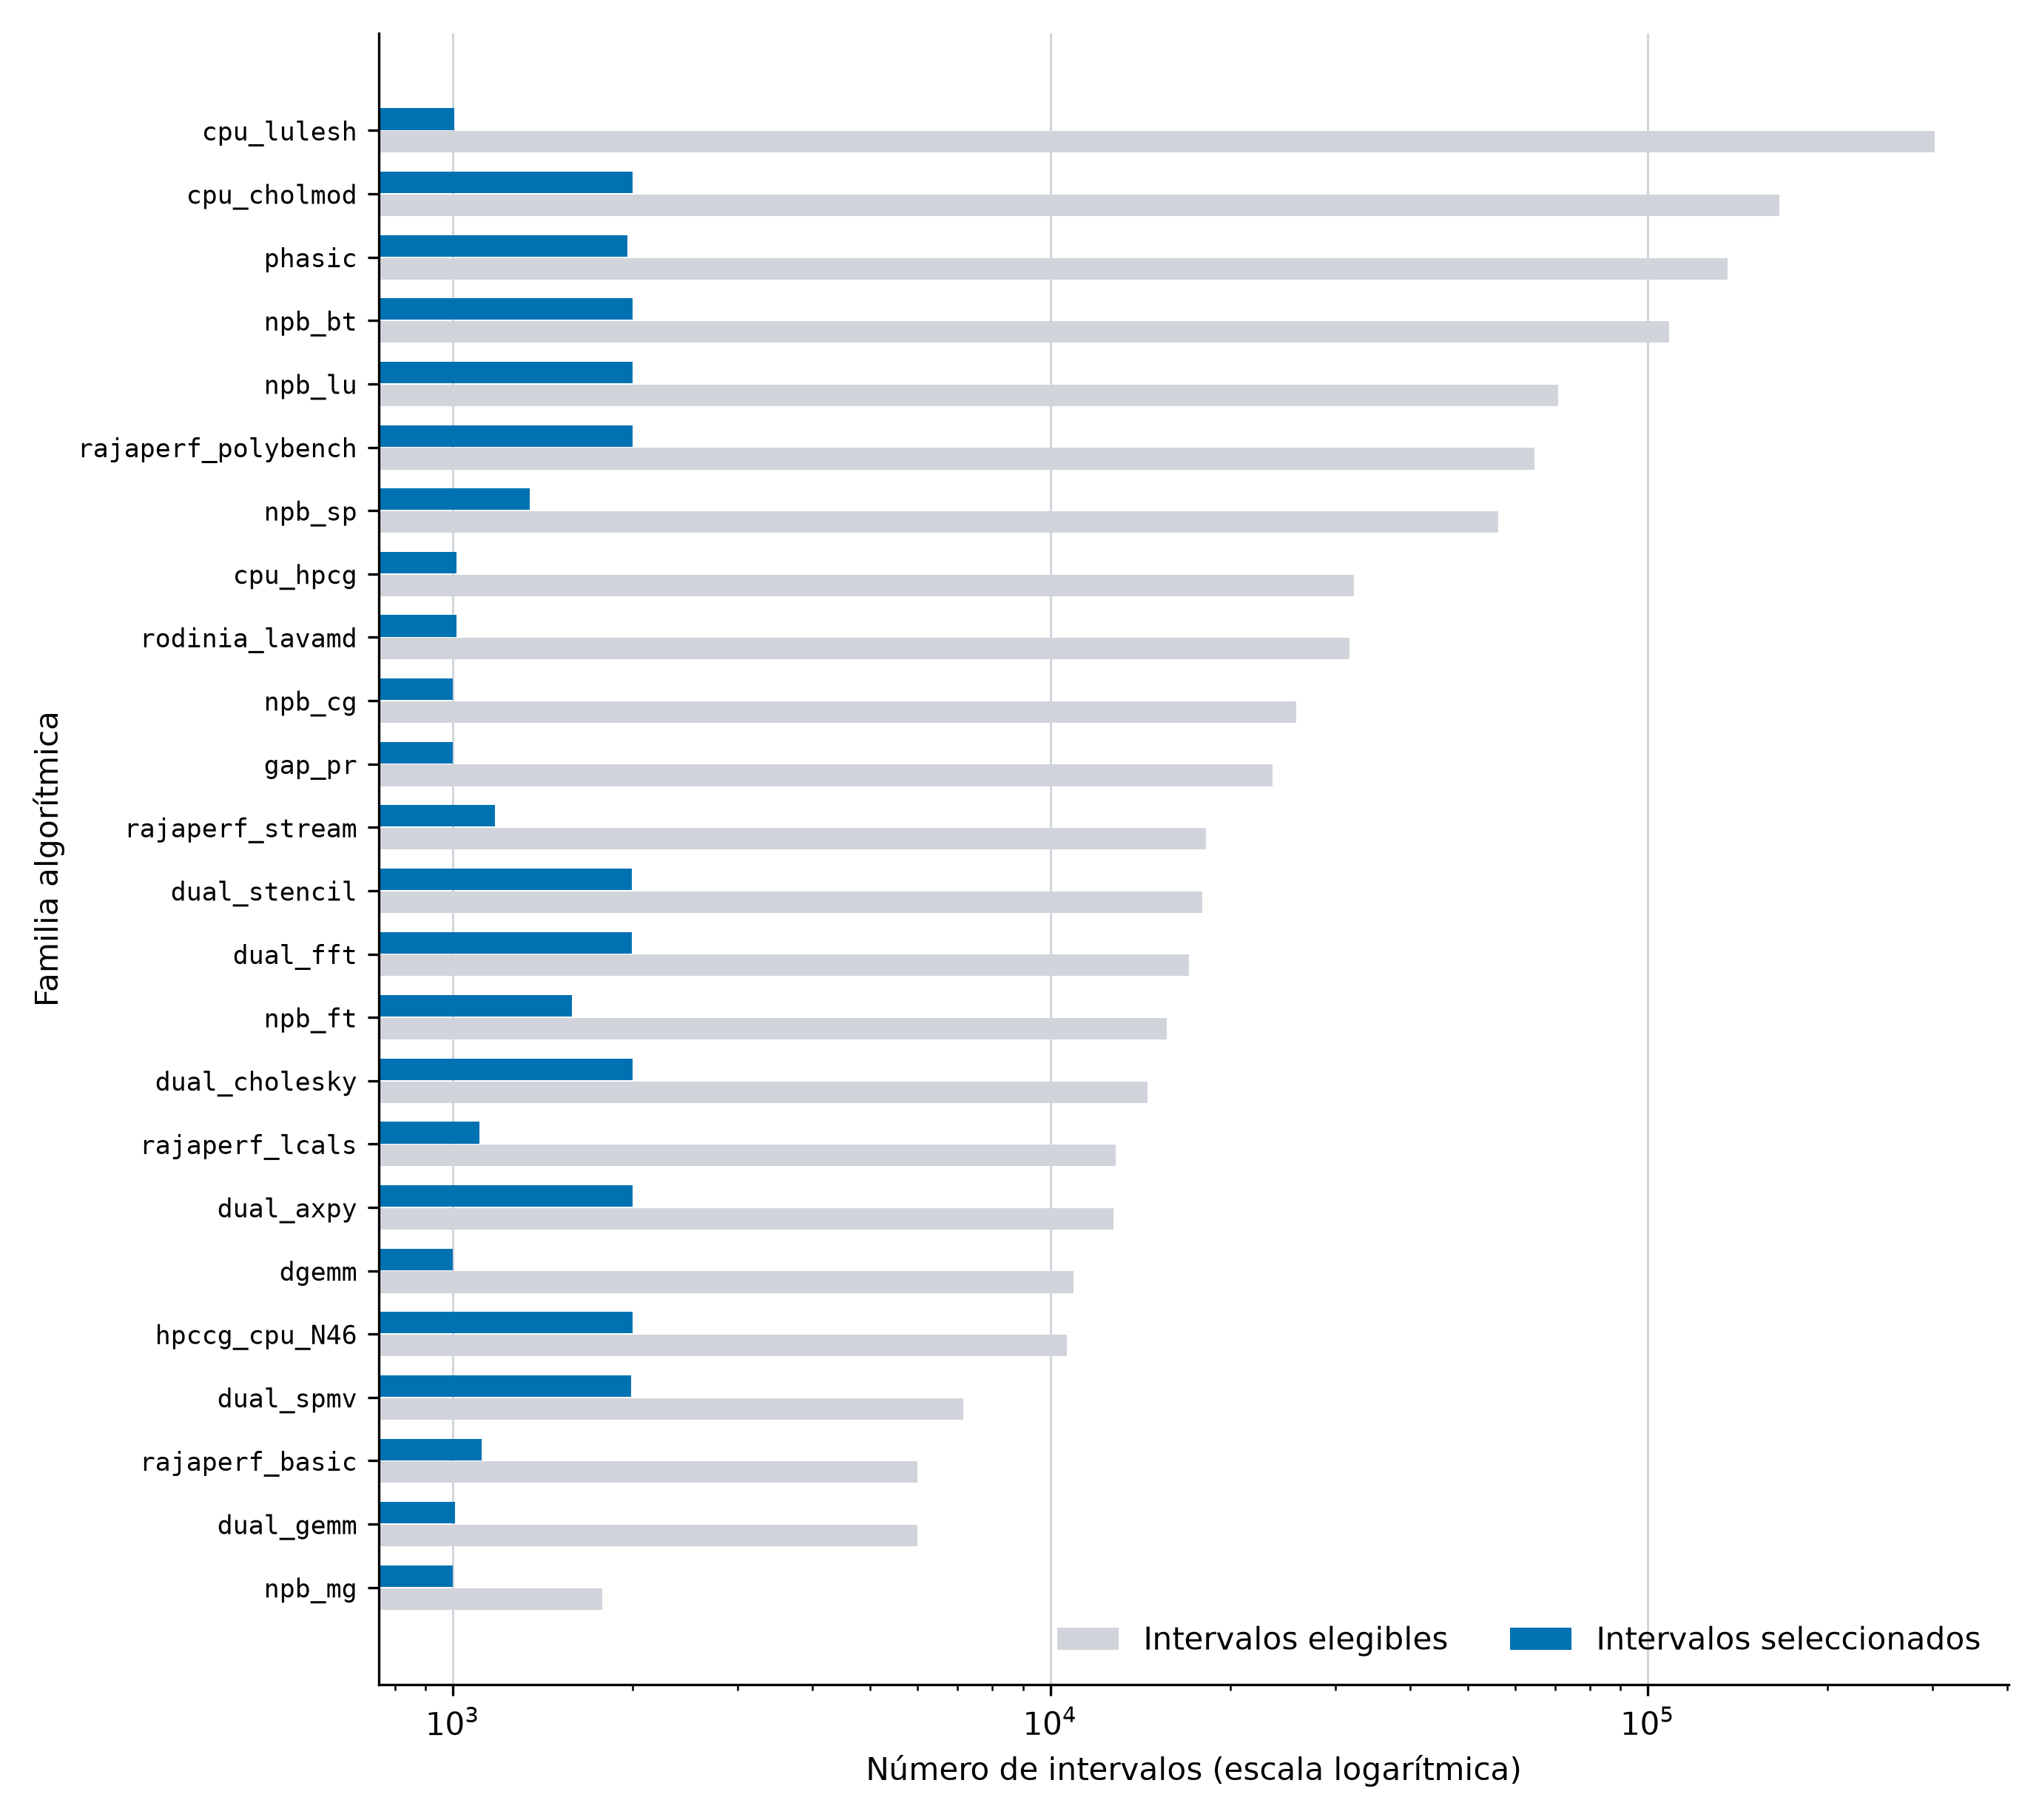
\includegraphics[width=0.92\textwidth]{figuras/fig_cpu_muestreo_familia_20260918.png}
    \caption[Muestreo estratificado del conjunto CPU]{Intervalos elegibles y seleccionados por familia algorítmica. El eje logarítmico permite comparar familias cuyo volumen original difiere en varios órdenes de magnitud. Fuente: elaboración propia.}
    \label{fig:cpu-muestreo-familia}
\end{figure}

\subsubsection{Variables de entrada}
\label{sec:resultados-cpu-entradas}

El modelo usa las seis variables de la Tabla \ref{tab:cpu-features-modelo}: cinco tasas normalizadas calculadas con los contadores del intervalo y la frecuencia física observada.

\begin{table}[H]
\centering
\caption{Variables de entrada del candidato CPU congelado.}
\label{tab:cpu-features-modelo}
\footnotesize
\setlength{\tabcolsep}{3pt}
\begin{tabular}{@{}p{3.6cm}p{4.6cm}p{4.8cm}@{}}
\toprule
\textbf{Variable} & \textbf{Cálculo} & \textbf{Interpretación} \\
\midrule
\texttt{ipc} & $N_{\mathrm{inst}}/N_{\mathrm{cyc}}$ & Trabajo retirado por ciclo \\
\texttt{mpki} & $1000N_{\mathrm{miss}}/N_{\mathrm{inst}}$ & Fallos de caché por millar de instrucciones \\
\texttt{cache\_miss\_rate} & $N_{\mathrm{miss}}/N_{\mathrm{ref}}$ & Fracción de referencias que fallan \\
\texttt{stall\_mem\_ratio} & $N_{\mathrm{stall}}/N_{\mathrm{cyc}}$ & Fracción de ciclos detenidos por memoria \\
\texttt{ips} & $N_{\mathrm{inst}}/\Delta t$ & Tasa de instrucciones del intervalo \\
\texttt{freq\_khz\_observed} & Mediana de las lecturas cubiertas & Frecuencia física observada \\
\bottomrule
\end{tabular}
\end{table}

Quedaron fuera las columnas con las que se calcula la etiqueta (FLOPs, bytes de DRAM, intensidad operacional y \textit{ridge}), porque con ellas el modelo no predeciría la etiqueta sino que la calcularía; los identificadores de kernel, nivel y repetición, que permiten reconocer la carga en lugar de su régimen; las señales de calidad del contador, que describen la adquisición y no la carga; y los deltas crudos, que dependen de la duración del intervalo y son redundantes frente a sus tasas.

La auditoría de correlación (sección \ref{sec:metodologia-correlacion-cpu}) se calculó sobre las doce columnas candidatas, antes de descartar las seis redundantes (Figura \ref{fig:cpu-correlacion-entradas}): el par más alto es 0.89 (Pearson), entre MPKI y las referencias de caché por millar de instrucciones, dos normalizaciones distintas de la misma señal de fallos de caché, y de ese par se retuvo MPKI. Sobre el vector final de seis variables, ningún par supera ya la correlación de 0.85: la correlación absoluta más alta es 0.74 (de Spearman), negativa, entre IPC y la fracción de ciclos detenidos por memoria, y la siguiente es 0.72 entre IPC e IPS. El factor de inflación de la varianza máximo es 5.5 con la correlación de Pearson y 7.3 con la de rangos, ambos de IPC, por debajo del umbral de alerta de 10, de modo que no fue necesario retirar ninguna variable adicional.

\begin{figure}[H]
    \centering
    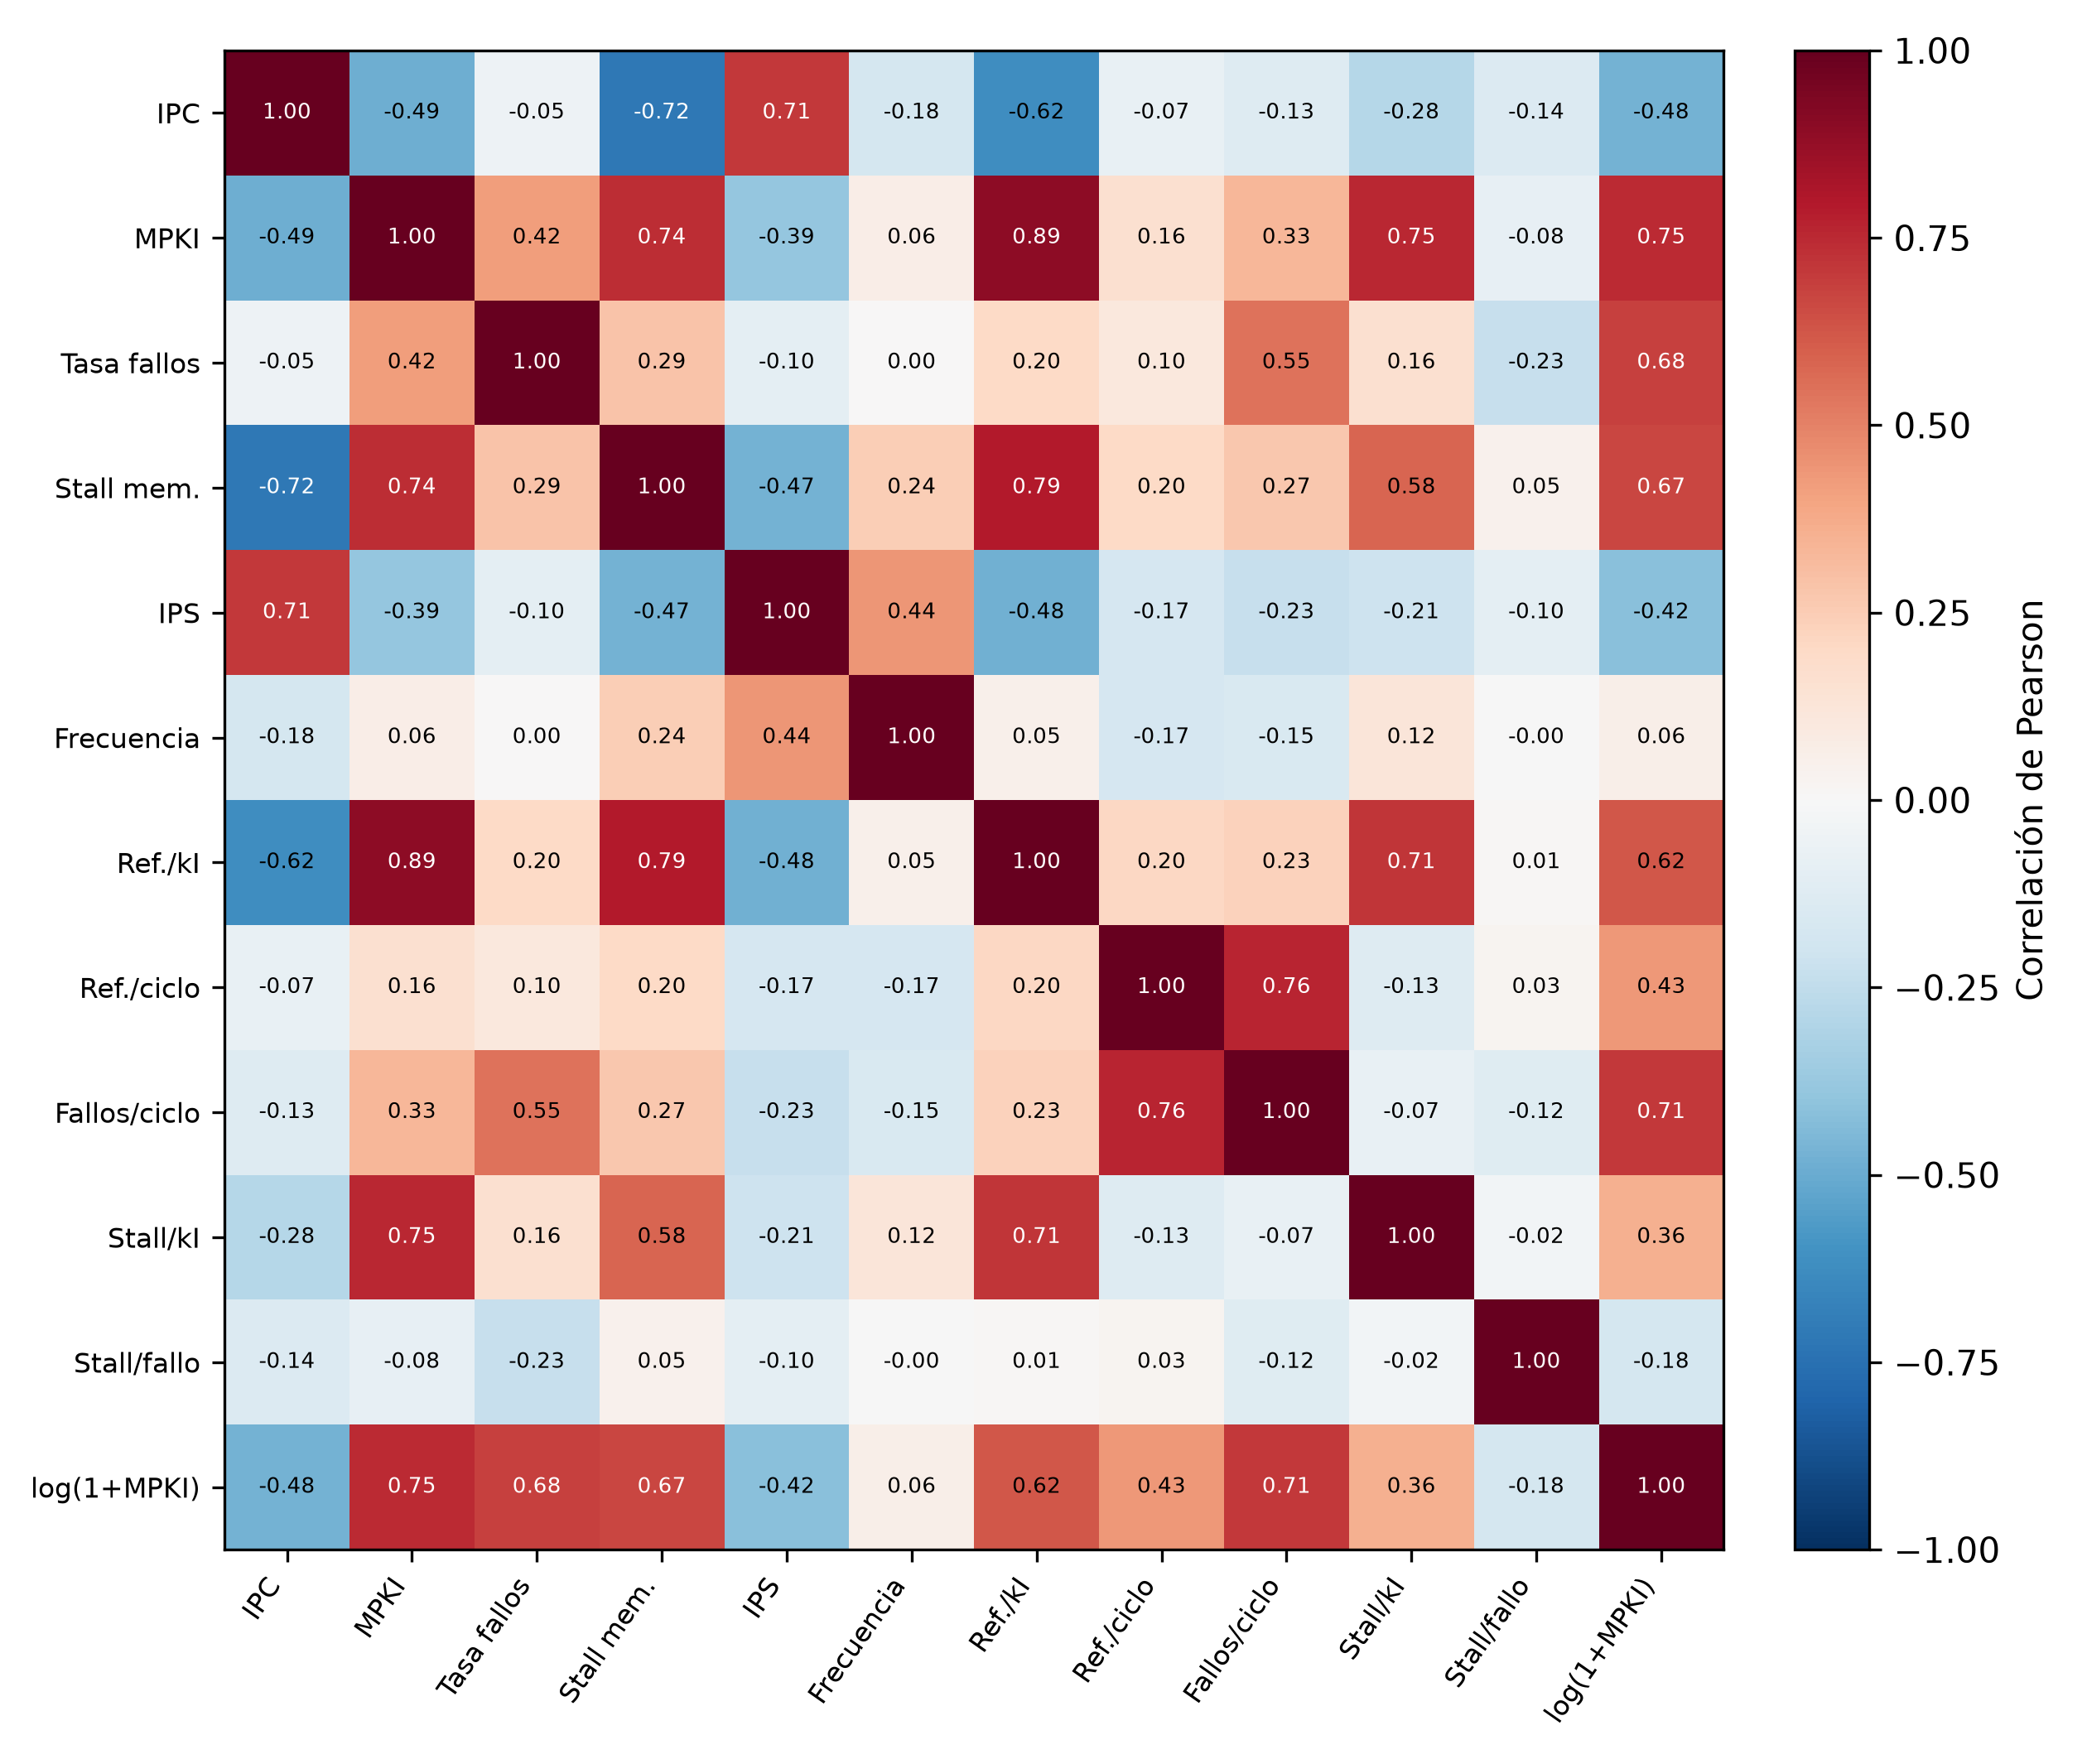
\includegraphics[width=0.72\textwidth]{figuras/fig_cpu_correlacion_entradas_20260918.png}
    \caption[Correlación entre las variables candidatas del clasificador CPU]{Correlación de Pearson entre las doce columnas candidatas, sobre los 1\,309\,755 intervalos elegibles, calculada antes de la selección del vector final de seis variables. Los pares más altos (MPKI con las dos normalizaciones de referencias de caché, 0.89 y 0.75) motivan retirar las columnas derivadas y conservar la medición más directa. Fuente: elaboración propia.}
    \label{fig:cpu-correlacion-entradas}
\end{figure}

Ampliar el vector de seis a doce entradas redundantes cambió la exactitud balanceada de 0.728 a 0.724 (IC95 de la diferencia, $-0.026$ a $+0.011$; Tabla \ref{tab:cpu-variantes-entrada}). Por ello se conservaron seis variables. La redundancia perjudicó más a la regresión logística, sin ofrecer a XGBoost una mejora medible de inferencia o precisión.

La frecuencia observada podría servir de atajo para deducir la etiqueta, porque el \textit{ridge} depende de ella. No ocurre: un modelo que solo la recibe alcanza 0.592, apenas por encima del azar, y retirarla del vector completo reduce el resultado solo 0.008 (IC95 de $-0.018$ a $+0.001$). En términos prácticos, el clasificador es un detector de presión sobre la jerarquía de memoria: al permutarlas, las variables que más deterioran el resultado son MPKI (0.055), la tasa de fallos de caché (0.038) y, en menor medida, la frecuencia (0.021), de modo que las seis columnas contienen bastante menos información que seis variables independientes.




\subsubsection{Selección de modelo e hiperparámetros}
\label{sec:resultados-cpu-modelo}

La Tabla \ref{tab:cpu-comparacion-modelos} y la Figura \ref{fig:cpu-comparacion-modelos} comparan los candidatos con hiperparámetros fijos, cinco semillas y el mismo protocolo LOFO. XGBoost, Extra Trees y Random Forest quedan dentro del mismo intervalo de incertidumbre; la regresión logística rinde menos. Se seleccionó XGBoost por su menor latencia entre los modelos de árboles, más de trece veces inferior a la de los dos bosques.

\begin{table}[H]
\centering
\caption{Comparación de modelos con hiperparámetros fijos, los seis a su vector final de seis variables. La sensibilidad de cada modelo al tamaño del vector de entrada se reporta por separado en la Tabla \ref{tab:cpu-variantes-entrada}. La latencia corresponde a una fila y un hilo, medida en el nodo de destino (paccaA100) con el proceso fijado a cuatro núcleos.}
\label{tab:cpu-comparacion-modelos}
\small
\setlength{\tabcolsep}{3pt}
\begin{tabular}{@{}p{3.9cm}>{\centering\arraybackslash}p{1.7cm}>{\centering\arraybackslash}p{2.8cm}>{\centering\arraybackslash}p{1.5cm}>{\centering\arraybackslash}p{1.8cm}@{}}
\toprule
\textbf{Modelo} & \textbf{Exact. bal.} & \textbf{IC95} & \textbf{F1 macro} & \textbf{Latencia p99} \\
\midrule
Regla mayoritaria & 0.464 & 0.423 a 0.492 & 0.205 & -- \\
Árbol de profundidad 1 & 0.630 & 0.566 a 0.700 & 0.713 & 109~\textmu s \\
Regresión logística & 0.680 & 0.618 a 0.742 & 0.765 & 475~\textmu s \\
Extra Trees & 0.732 & 0.666 a 0.804 & 0.717 & 5477~\textmu s \\
Random Forest & 0.737 & 0.675 a 0.803 & 0.763 & 5453~\textmu s \\
\textbf{XGBoost} & \textbf{0.728} & 0.669 a 0.790 & 0.760 & 404~\textmu s \\
\bottomrule
\end{tabular}
\end{table}

\begin{figure}[H]
    \centering
    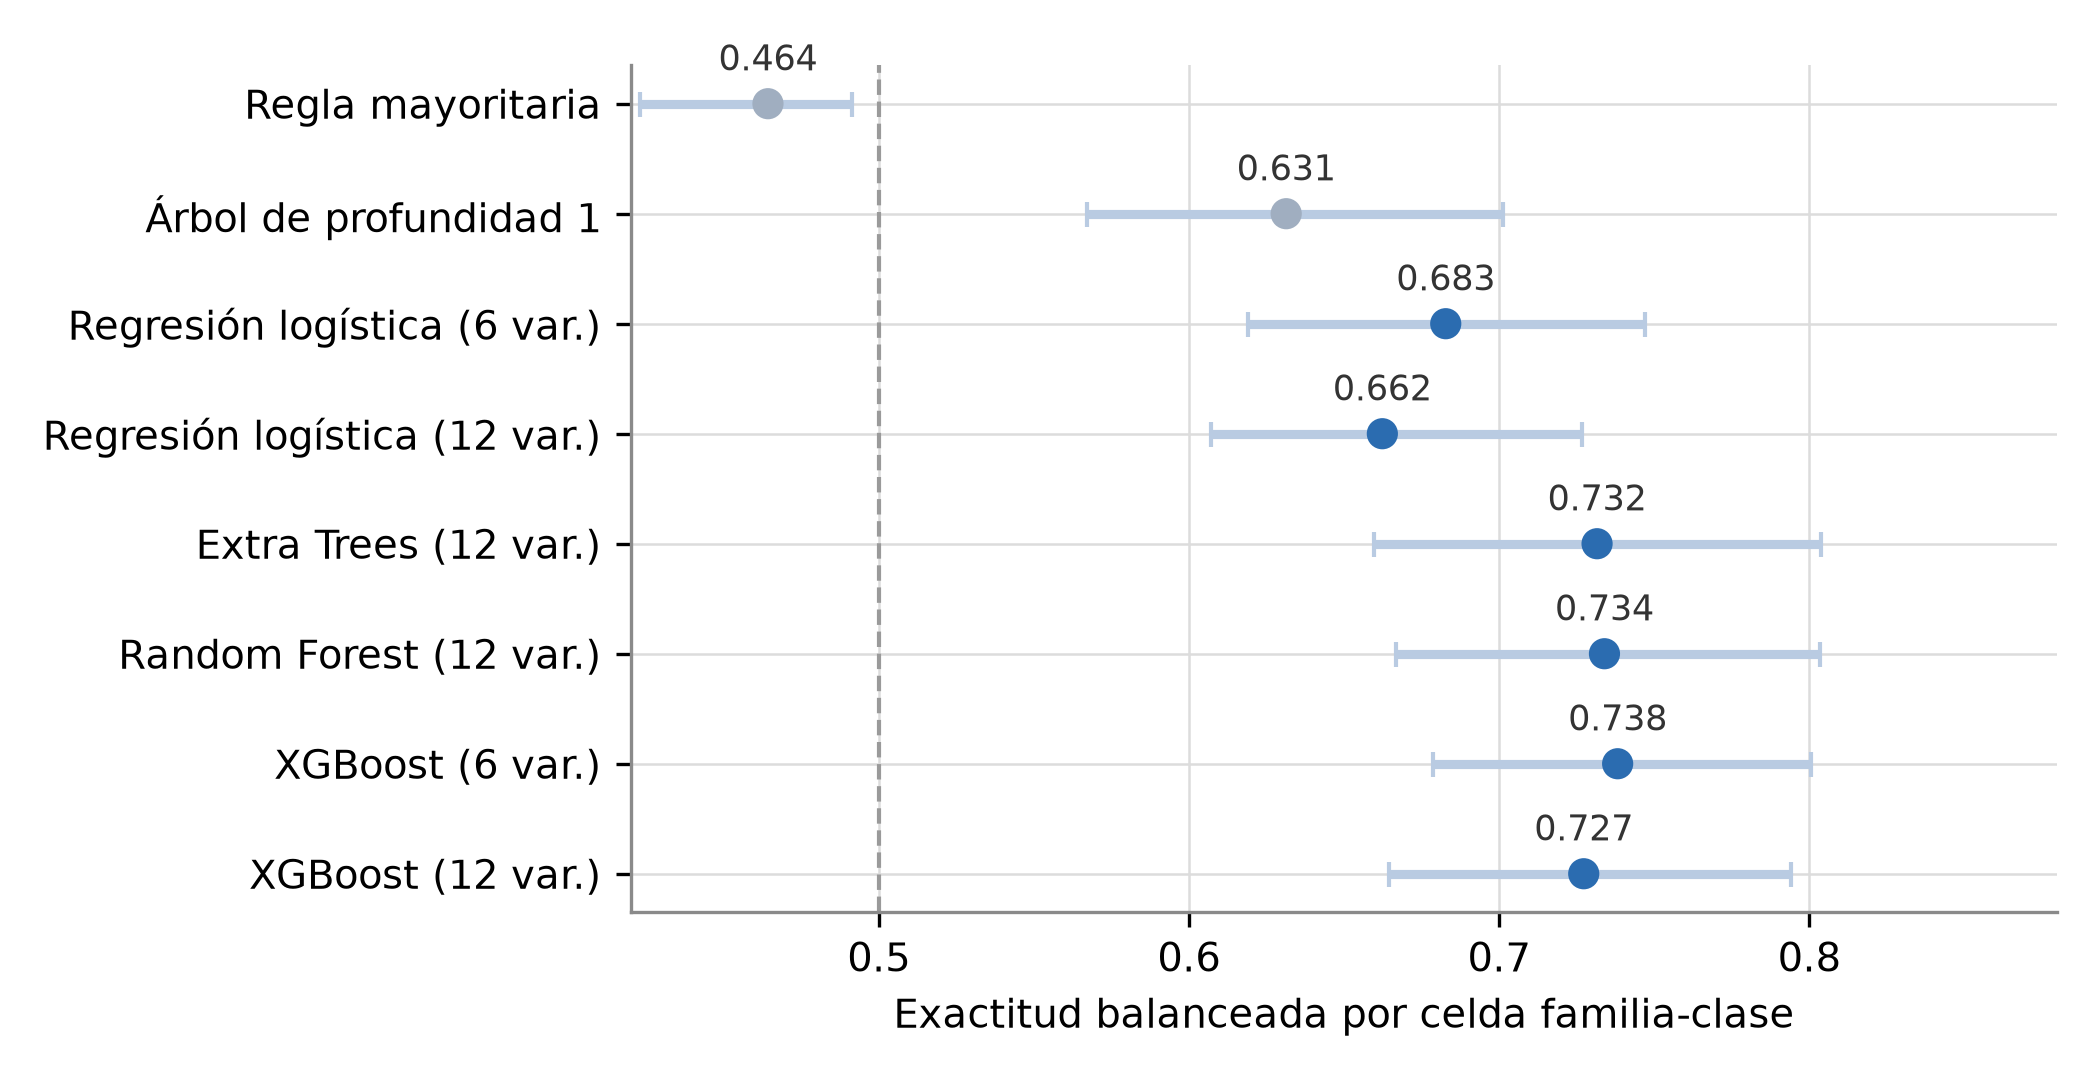
\includegraphics[width=0.92\textwidth]{figuras/fig_cpu_comparacion_modelos_20260919.png}
    \caption[Comparación de modelos del clasificador CPU]{Exactitud balanceada por celda de familia y clase de cada modelo, con intervalo de confianza del 95\% obtenido por remuestreo de las 30 familias. Los intervalos se solapan entre todos los modelos con capacidad suficiente. Fuente: elaboración propia.}
    \label{fig:cpu-comparacion-modelos}
\end{figure}

\paragraph{Búsqueda de hiperparámetros.} Sobre esa base se ejecutó una búsqueda con el muestreador TPE de Optuna \cite{Akiba2019}, anidada dentro de cada pliegue: con la familia retirada apartada, se puntúan las configuraciones con un LOFO interno sobre las 29 restantes, se ajusta la mejor y solo entonces se evalúa la familia retirada. La anidación impide que el resultado se infle por escoger la configuración que mejor se ajusta a la familia reportada. Se evaluaron 15 configuraciones por pliegue para XGBoost y 8 para la regresión logística.

Para XGBoost la búsqueda no mejora de forma distinguible la configuración fija: la diferencia pareada por familia es de $+0.019$, con un intervalo de confianza del 95\% de $-0.007$ a $+0.050$ que incluye el cero (14 familias mejoran, 8 empeoran, de 30). Para la regresión logística el efecto es, en cambio, estadísticamente distinguible de cero (IC95 de $+0.0004$ a $+0.0042$; 5 familias mejoran, 2 empeoran), pero de una magnitud irrelevante, $+0.002$: la búsqueda encuentra una configuración mejor de forma consistente, no por azar, y aun así no cambia en ninguna medida práctica el modelo desplegable. El puntaje interno de cada pliegue se mueve en un rango estrecho (de 0.734 a 0.761) mientras el resultado externo va de 0.487 a 1.000, de modo que el criterio interno no distingue configuraciones buenas de malas para una familia nueva. Por eso se conservó la configuración fija de XGBoost, que además es la más simple de reproducir. La conclusión, coherente con la comparación de modelos y con las variantes del vector de entrada, es que el desempeño no está limitado por la capacidad del modelo ni por el ajuste de sus hiperparámetros.



La configuración congelada es la de la Tabla \ref{tab:cpu-configuracion-final}.


\subsubsection{Métricas de evaluación}
\label{sec:resultados-cpu-metricas}
\label{sec:resultados-cpu-protocolo}

\paragraph{Esquema de evaluación.} Un \emph{pliegue} consiste en retirar una familia completa, ajustar el modelo con las 29 restantes y clasificar después los intervalos de la familia retirada. El procedimiento se repite 30 veces, una por familia, y ningún intervalo de la familia evaluada interviene en el ajuste ni en ninguna decisión de diseño. Responde la pregunta operativa pertinente: si el agente encuentra un algoritmo que nunca vio, ¿acierta su régimen? La alternativa más débil, acertar sobre otra ejecución de un algoritmo ya conocido, da resultados muy distintos con el mismo modelo y los mismos datos (Tabla \ref{tab:cpu-protocolos}): repartir intervalos al azar produce 0.874, porque dos intervalos consecutivos de una misma corrida son casi idénticos y el modelo reconoce la carga en lugar de su régimen. Todas las cifras de este capítulo corresponden a dejar una familia fuera.



\paragraph{Qué es una celda.} Una \emph{celda} es la combinación de una familia algorítmica y una clase de fase; por ejemplo, los intervalos \textit{compute-bound} de \texttt{cpu\_cholmod} forman una celda y sus intervalos \textit{memory-bound} forman otra. El conjunto tiene 56 celdas: 30 familias por dos clases son 60 combinaciones, de las cuales cuatro están vacías porque esa familia nunca presenta esa clase. Cada celda tiene su tamaño, de 5 a más de 300\,000 intervalos, y su fracción de aciertos (Figura \ref{fig:cpu-celdas}).

\begin{figure}[H]
    \centering
    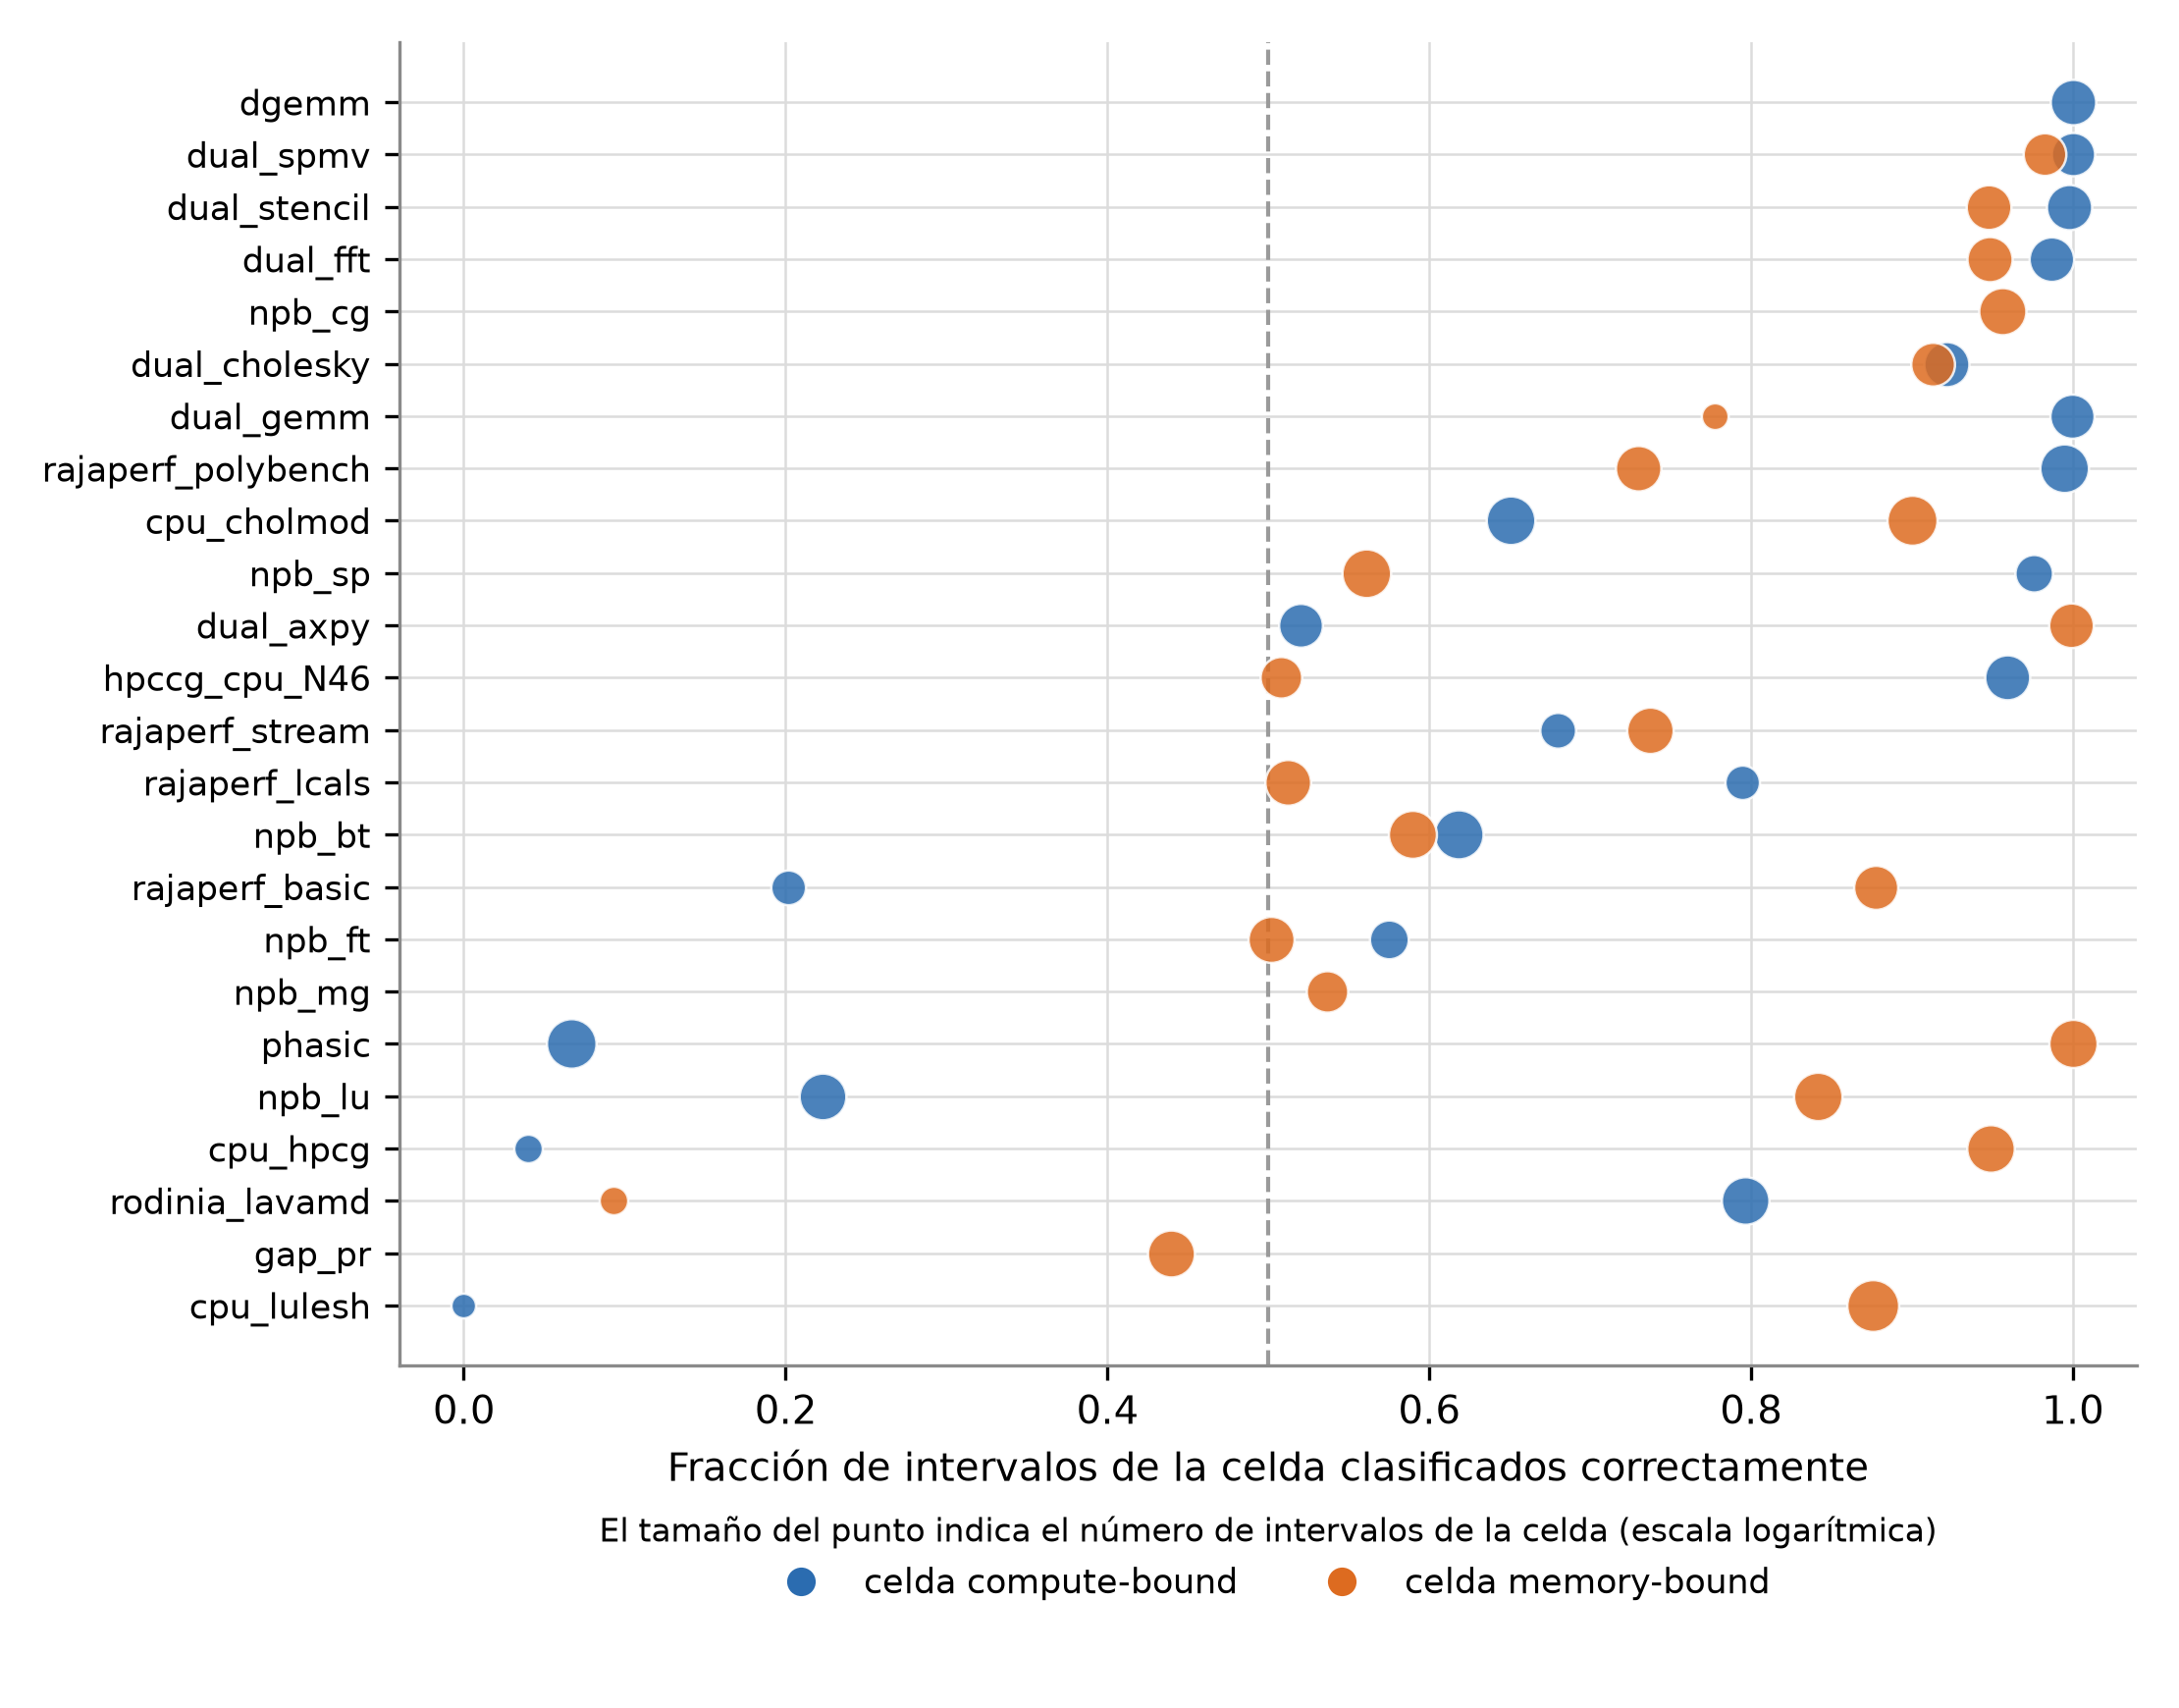
\includegraphics[width=0.94\textwidth]{figuras/fig_cpu_celdas_20260919.png}
    \caption[Acierto del modelo final en cada celda de familia y clase]{Fracción de aciertos del modelo final en cada una de las 56 celdas de familia y clase, con evaluación sobre todos los intervalos de la familia retirada. Las familias con una sola celda son las de una sola clase. Fuente: elaboración propia.}
    \label{fig:cpu-celdas}
\end{figure}

\paragraph{Métricas empleadas.} La Tabla \ref{tab:cpu-metricas-definicion} define las nueve métricas. Para una clase $c$, $\mathrm{VP}_c$ son los intervalos de esa clase correctamente clasificados, $\mathrm{FP}_c$ los de otra clase clasificados como $c$ y $\mathrm{FN}_c$ los de $c$ clasificados como otra clase. Las ocho primeras agrupan todos los intervalos y por ello pesan cada familia según su volumen; la última pesa cada celda por igual.



\paragraph{Por qué la exactitud por celda es la métrica principal.} No depende del volumen, de modo que una corrida larga no decide el resultado; no depende de la proporción entre clases dentro de una familia; y está definida también para las cuatro familias de una sola clase (\texttt{dgemm}, \texttt{gap\_pr}, \texttt{npb\_cg} y \texttt{npb\_mg}), donde el F1 macro calculado dentro de cada familia queda acotado a 0.5 aunque todos sus intervalos se clasifiquen bien. La Tabla \ref{tab:cpu-metricas-valores} reúne todas las métricas del modelo final sin abstención.



La exactitud balanceada clásica (0.760) y la F1 macro agrupada (0.760) coinciden entre sí; la exactitud por celda (0.728) queda unos tres puntos por debajo porque, al pesar cada celda por igual, castiga las celdas de muy pocos intervalos en las que el modelo falla. La exactitud global de 0.769 es la más alta de las tres, pero es la que más depende de la composición del conjunto y no debe leerse como la capacidad del modelo.

\paragraph{Límite de la métrica.} La exactitud por celda asigna el mismo peso a una celda de 5 intervalos que a una de 300\,000. Diez de las 56 celdas tienen menos de 100 intervalos evaluados: suman 128 intervalos y pesan 17.9\% de la métrica; excluirlas la subiría de 0.728 a 0.777. Se conservan porque retirar celdas después de ver que fallan sería seleccionar datos por el resultado, y porque son informativas: muestran que las clases raras dentro de una familia casi pura no se reconocen.

\paragraph{Incertidumbre.} Se informan dos fuentes. La semilla del submuestreo se varió cinco veces. La composición del catálogo se evaluó mediante remuestreo con reemplazo de las 30 familias, con 2000 réplicas. Esta segunda fuente domina y es la que debe usarse al comparar configuraciones: con 30 familias, cualquier diferencia menor que 0.03 es indistinguible del ruido.


\subsubsection{Evaluación del modelo final}
\label{sec:resultados-cpu-final}

Se evaluó el modelo sobre los 1\,309\,755 intervalos elegibles, cada uno clasificado por el modelo del pliegue que no vio su familia, promediando las cinco semillas de muestreo. Si debe emitir siempre una clase, la exactitud balanceada por celda es 0.728, la F1 macro agrupada 0.760 y la exactitud global 0.769. La Tabla \ref{tab:cpu-metricas-clase} desagrega el resultado por clase y la Figura \ref{fig:cpu-matriz-confusion} muestra las matrices de confusión. En el promedio agrupado por intervalo, la sensibilidad de \textit{memory-bound} (0.806) supera en nueve puntos a la de \textit{compute-bound} (0.714); en el promedio por celda de familia y clase la diferencia se invierte y se estrecha (0.700 y 0.759, respectivamente). Ambos promedios describen la misma asimetría: los intervalos \textit{compute-bound} de una familia nueva se parecen más a intervalos \textit{memory-bound} de familias ya vistas que en sentido contrario (sección \ref{sec:resultados-cpu-limite}), y no al desbalance del ajuste, que está corregido por la ponderación.

\begin{figure}[H]
    \centering
    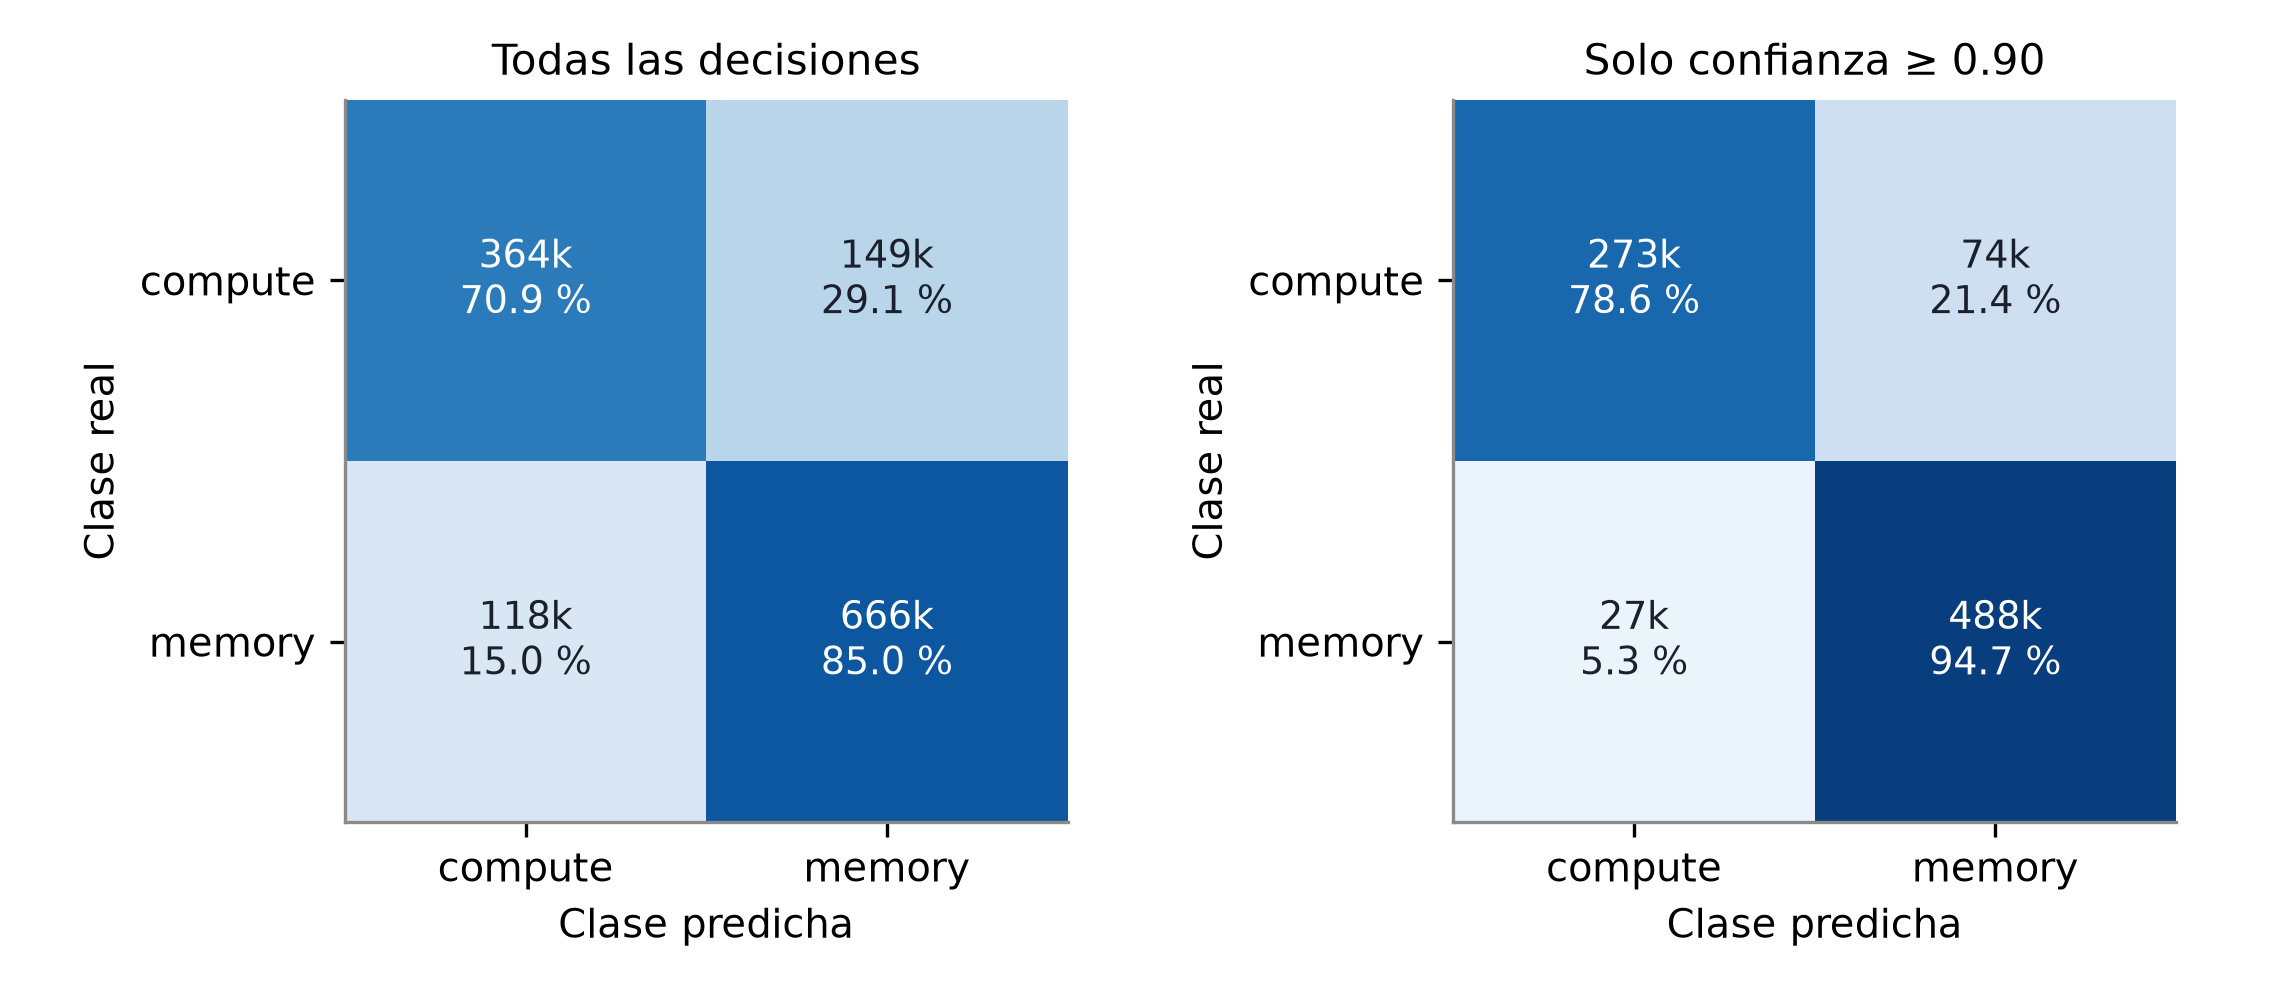
\includegraphics[width=0.94\textwidth]{figuras/fig_cpu_matriz_confusion_20260919.png}
    \caption[Matrices de confusión del clasificador CPU]{Matrices de confusión del modelo final. A la izquierda, cuando se obliga a emitir una clase en todos los intervalos; a la derecha, solo sobre los intervalos con confianza mayor o igual a 0.85. El porcentaje está calculado por fila, es decir, respecto de la clase real. Fuente: elaboración propia.}
    \label{fig:cpu-matriz-confusion}
\end{figure}

El resultado no es uniforme entre familias (Figura \ref{fig:cpu-resultado-familia}). Catorce familias superan 0.9 de exactitud y cinco quedan por debajo de 0.55, con \textit{npb\_ft} en 0.314. Las mejores son las de comportamiento extremo y estable; las peores, aquellas cuyo perfil de contadores coincide con el de familias de la clase contraria.

\begin{figure}[H]
    \centering
    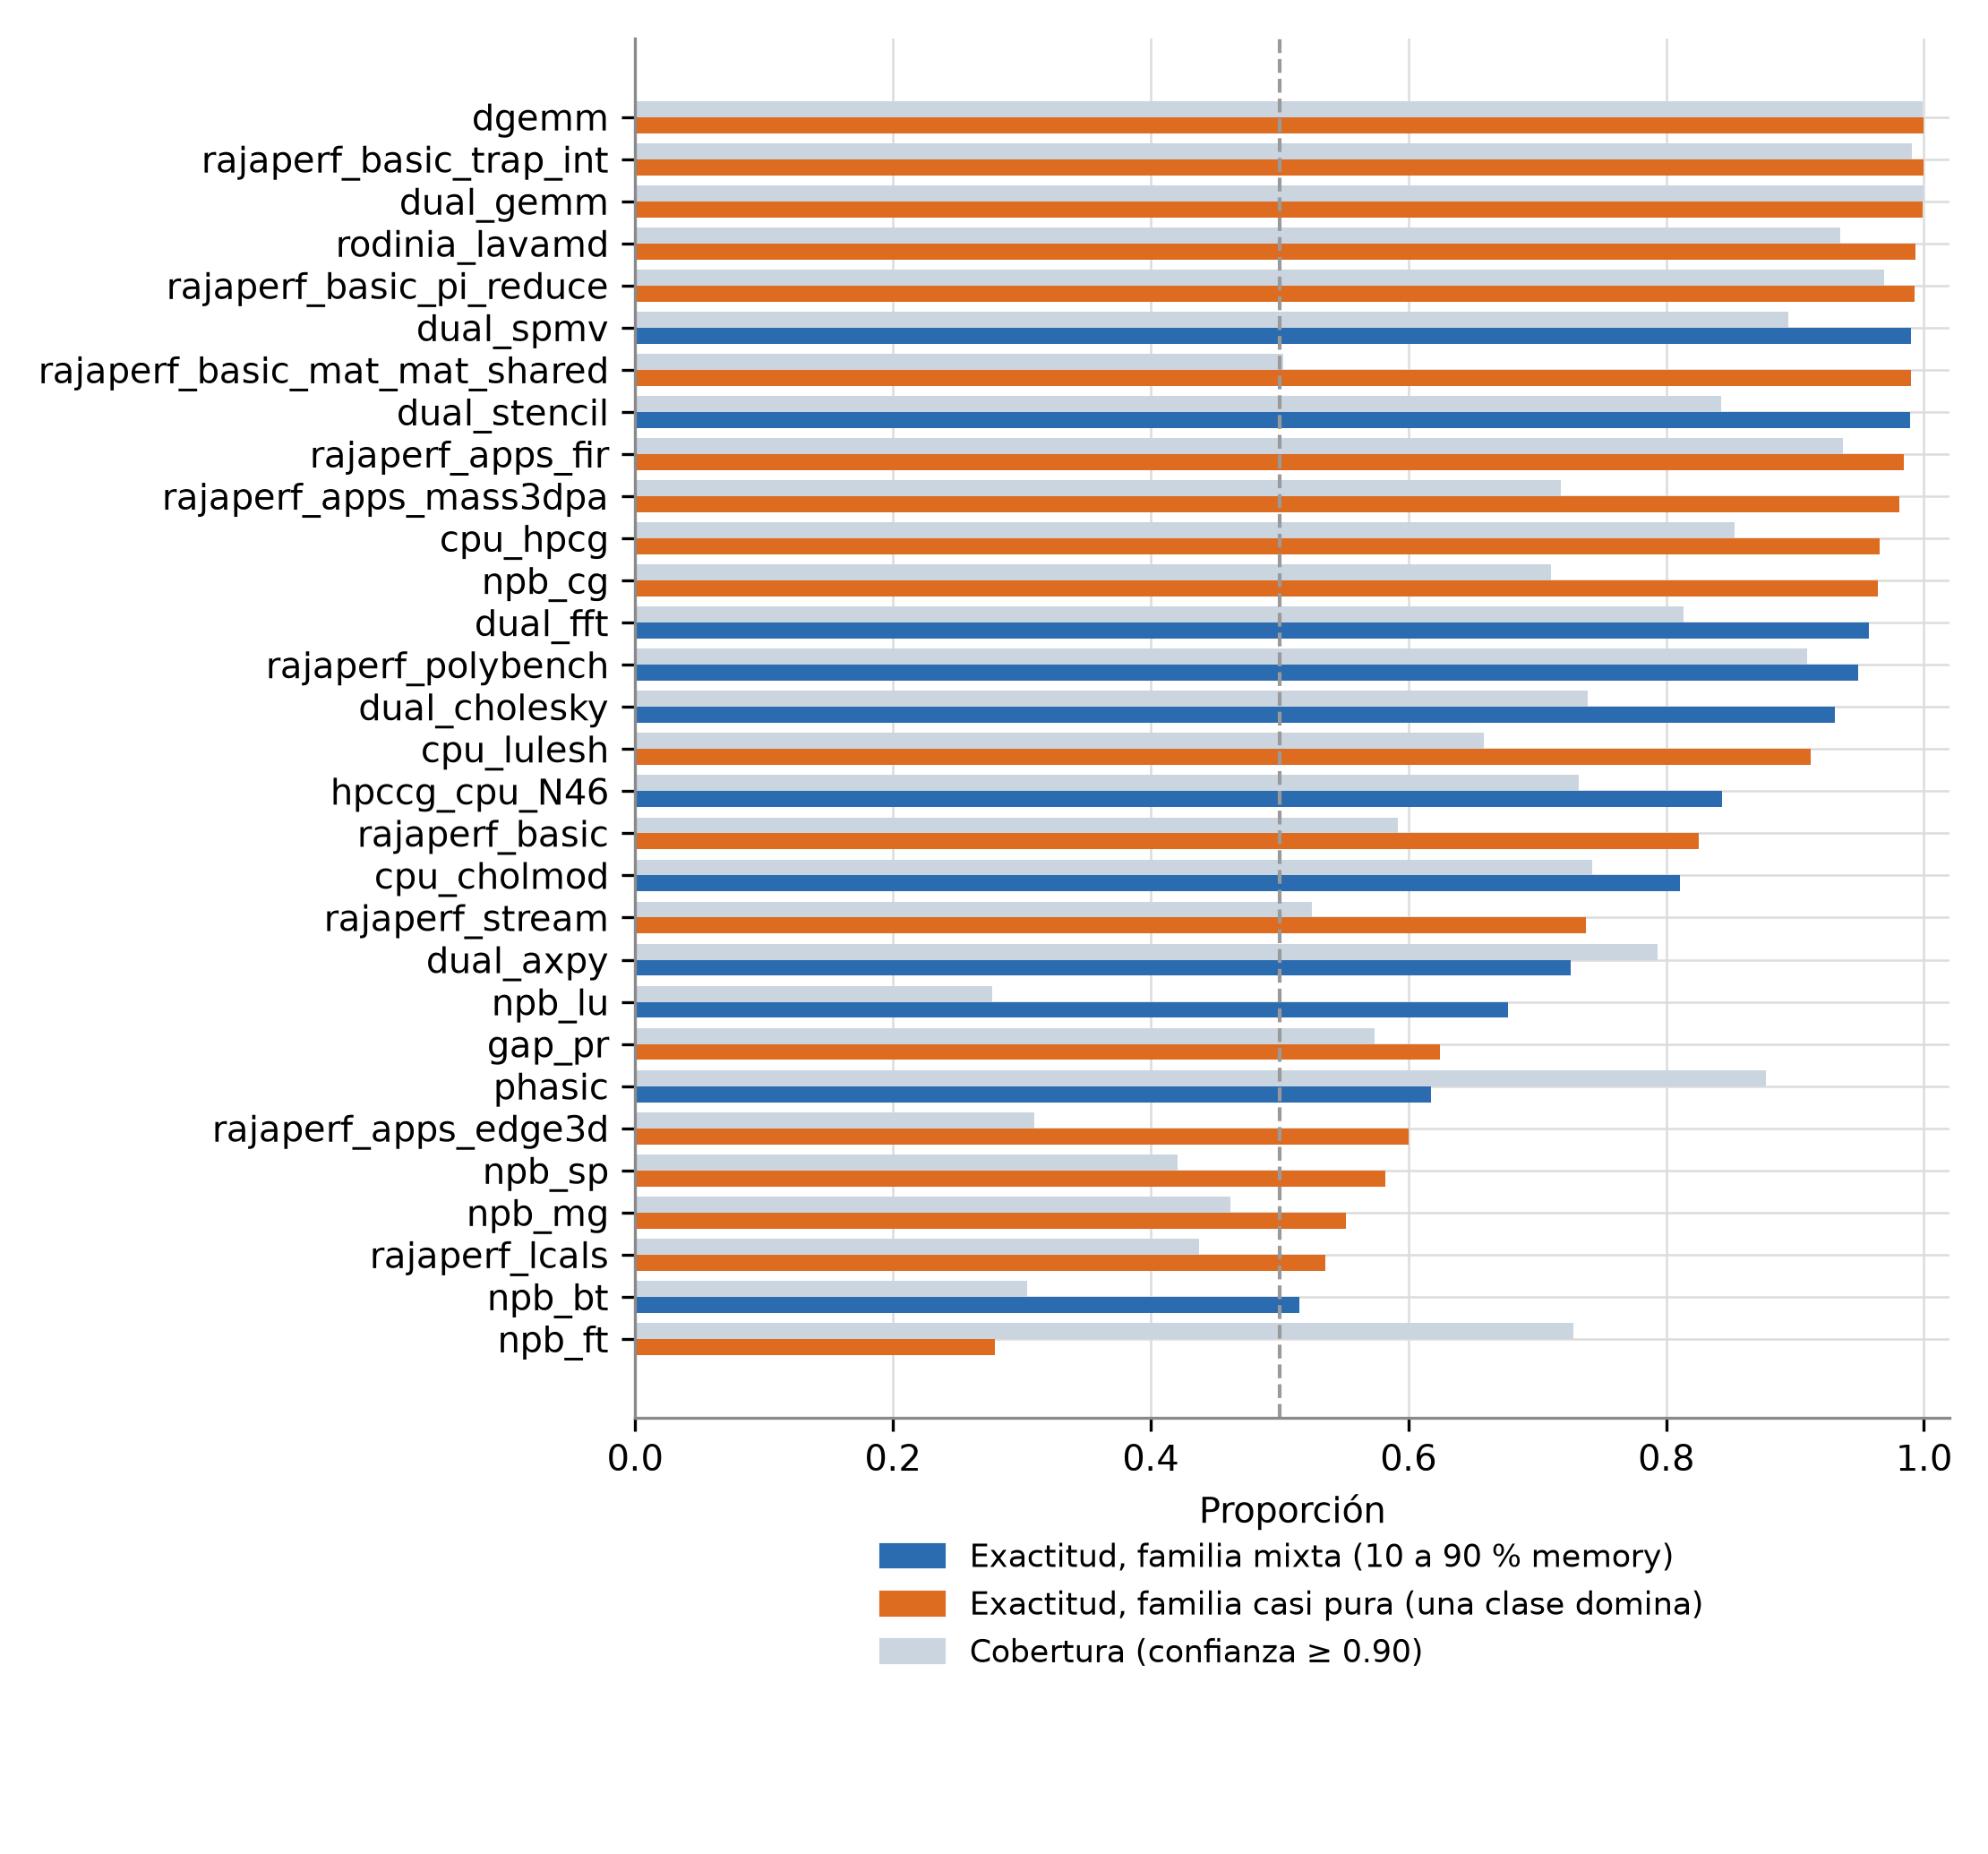
\includegraphics[width=0.94\textwidth]{figuras/fig_cpu_resultado_por_familia_20260919.png}
    \caption[Resultado del clasificador CPU por familia]{Exactitud del modelo final y cobertura de la decisión automática para cada familia retirada. El color distingue las familias mixtas (entre 10 y 90 \% de intervalos memory-bound) de las casi puras. Fuente: elaboración propia.}
    \label{fig:cpu-resultado-familia}
\end{figure}

La Figura \ref{fig:cpu-exactitud-cobertura-frecuencia} resume el desempeño por nivel. Por nivel de frecuencia, en la métrica principal el resultado va de 0.823 en el nivel nativo a 0.657 en F7 (Tabla \ref{tab:cpu-resultado-frecuencia}) y decrece, en general, al bajar el reloj. En los niveles bajos el \textit{ridge} desplaza más intervalos hacia la clase de cómputo (la fracción \textit{memory-bound} baja de 0.71 a 0.54) y la cobertura de la decisión automática cae de 0.85 a 0.64, lo que es consistente con que allí más intervalos quedan cerca de la frontera entre clases. La exactitud global repunta en F8 (0.757, frente a 0.710 en F7), pero ese repunte es casi enteramente un efecto de composición de clases: en la exactitud balanceada por celda, que no depende de cuántos intervalos aporta cada clase, F8 (0.659) queda prácticamente igualado con F7 (0.657) y no rebota. F8 es también el nivel con más intervalos (256\,531, frente a 85\,447--186\,309 en los demás), de modo que su exactitud global pesa más hacia la clase \textit{compute-bound} mayoritaria en ese régimen, que el modelo reconoce mejor a esa frecuencia.




\begin{figure}[H]
    \centering
    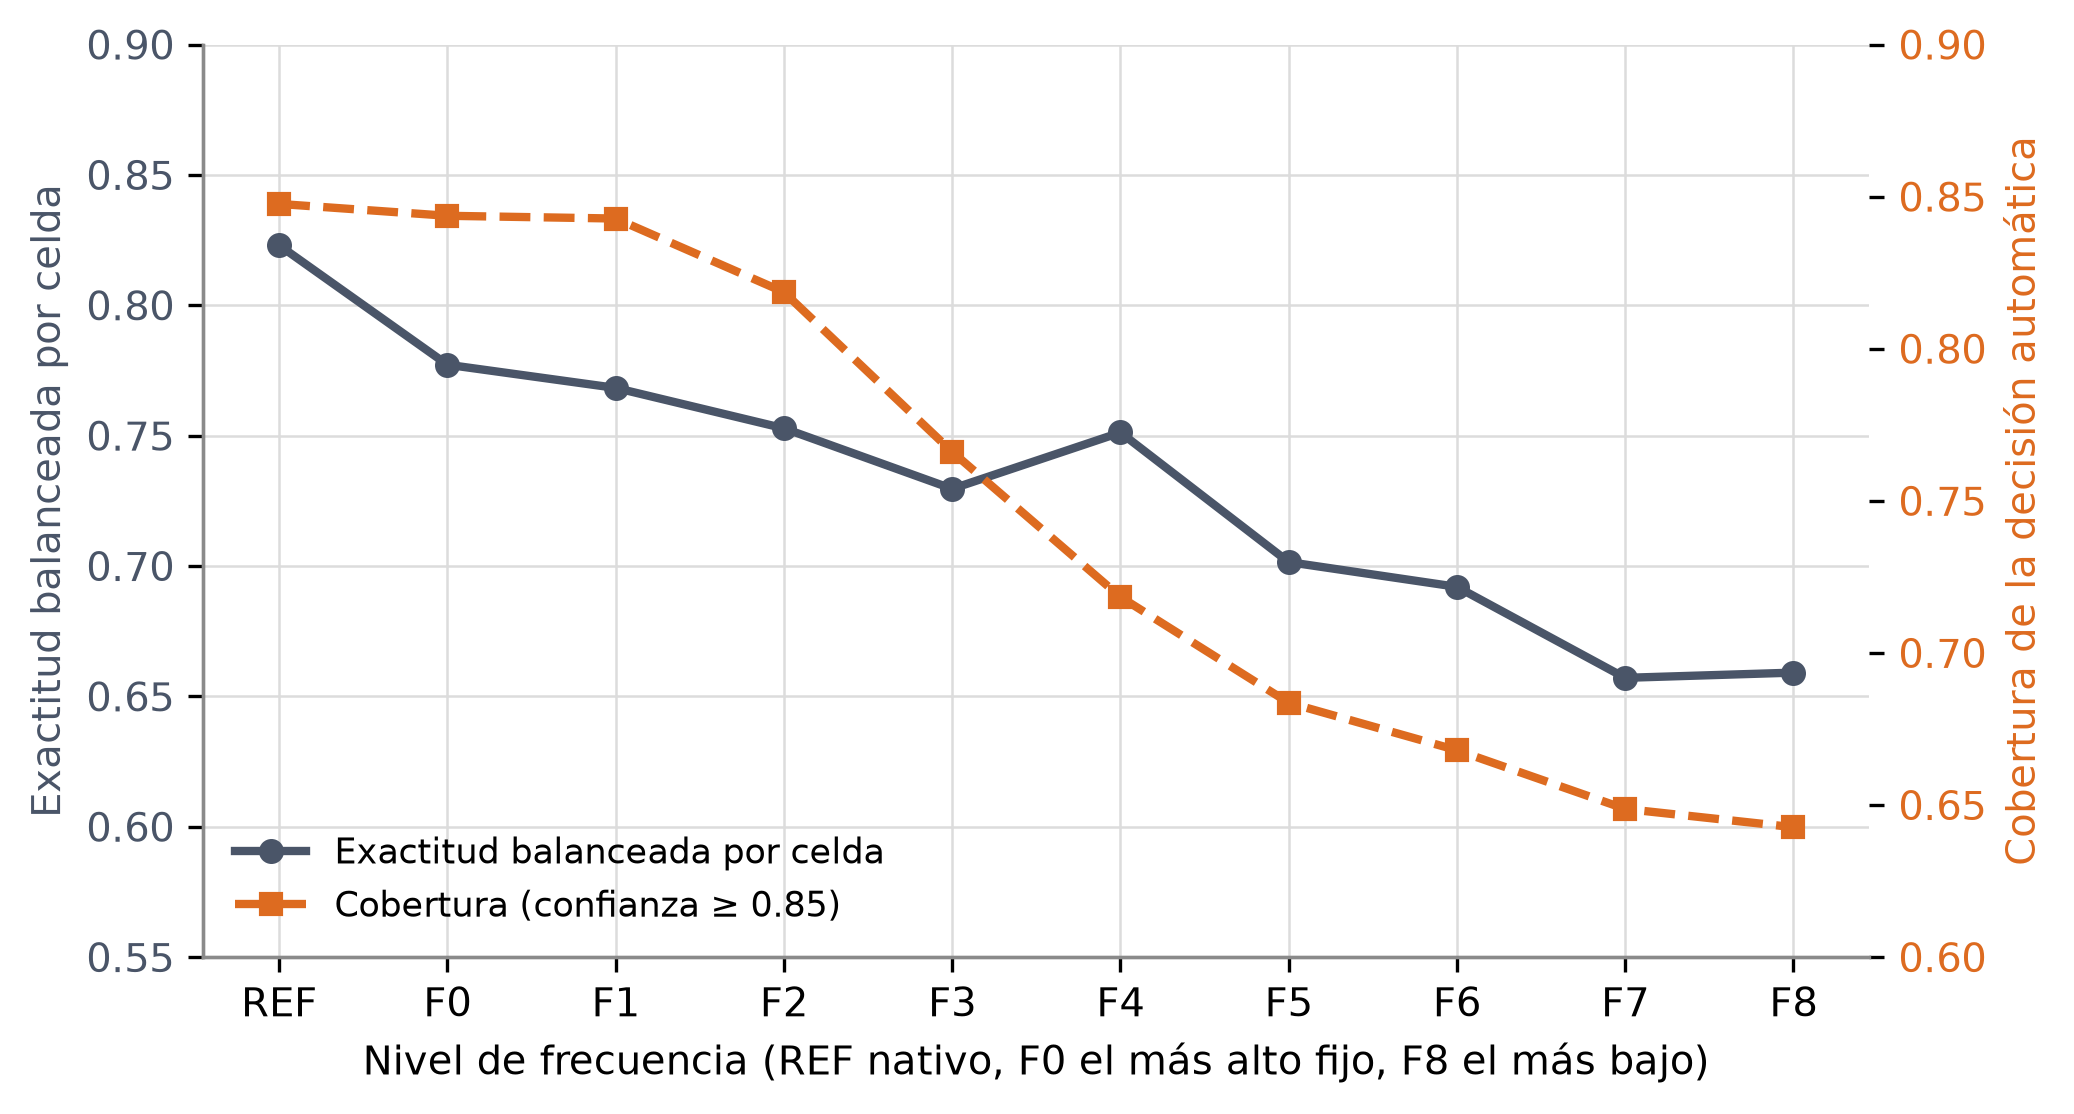
\includegraphics[width=0.78\textwidth]{figuras/fig_cpu_exactitud_cobertura_frecuencia_20260922.png}
    \caption[Exactitud y cobertura del clasificador CPU por nivel de frecuencia]{Exactitud balanceada por celda y cobertura de la decisión automática (confianza $\geq 0.85$) en función del nivel de frecuencia. Ambas caen de forma conjunta al bajar el reloj. Fuente: elaboración propia.}
    \label{fig:cpu-exactitud-cobertura-frecuencia}
\end{figure}

\subsubsection{Decisión selectiva y costo de inferencia}
\label{sec:resultados-cpu-selectiva}

El umbral de abstención CPU se eligió con LOFO interno y un piso de cobertura media por celda de 0.60 (Tabla \ref{tab:cpu-umbral-rejilla}). Aunque la rejilla proponía 0.90, se congeló 0.85: el aumento de exactitud de selección era solo de 0.003 y reducía la cobertura en 6.5 puntos. La evaluación externa del modelo ya congelado se presenta a continuación; el criterio interno y ese resultado no son la misma estimación.

Con el umbral 0.85 ya congelado, evaluado externamente sobre el modelo final, la cobertura es del 72.2\% de los intervalos (75.1\% promediando por familia); el resto recibe \textit{revisar}. Sobre lo que decide, la exactitud balanceada por celda sube de 0.728 a 0.738, la F1 macro agrupada de 0.760 a 0.842 y la sensibilidad de \textit{compute-bound} de 0.714 a 0.762 (Tabla \ref{tab:cpu-selectiva}); la ganancia por celda es modesta y la mayor parte de la mejora se ve en las métricas agrupadas. Abstenerse al azar en una proporción equivalente de intervalos deja la exactitud balanceada en 0.716 y la F1 macro en 0.752, sin mejora, de modo que la ganancia proviene de que la confianza identifica casos difíciles y no de decidir menos.





El límite de la abstención es que la confianza está mal calibrada fuera de la familia de entrenamiento (Figura \ref{fig:cpu-umbral-calibracion}): la confianza media declarada es 0.890 frente a una exactitud observada de 0.764, con un error de calibración esperado de 0.126. Hay familias que fallan \emph{con} confianza alta y a las que el umbral no protege: entre los intervalos con confianza mayor o igual a 0.9, \textit{npb\_ft} acierta el 32\% y \textit{npb\_mg} el 35\%.

\begin{figure}[H]
    \centering
    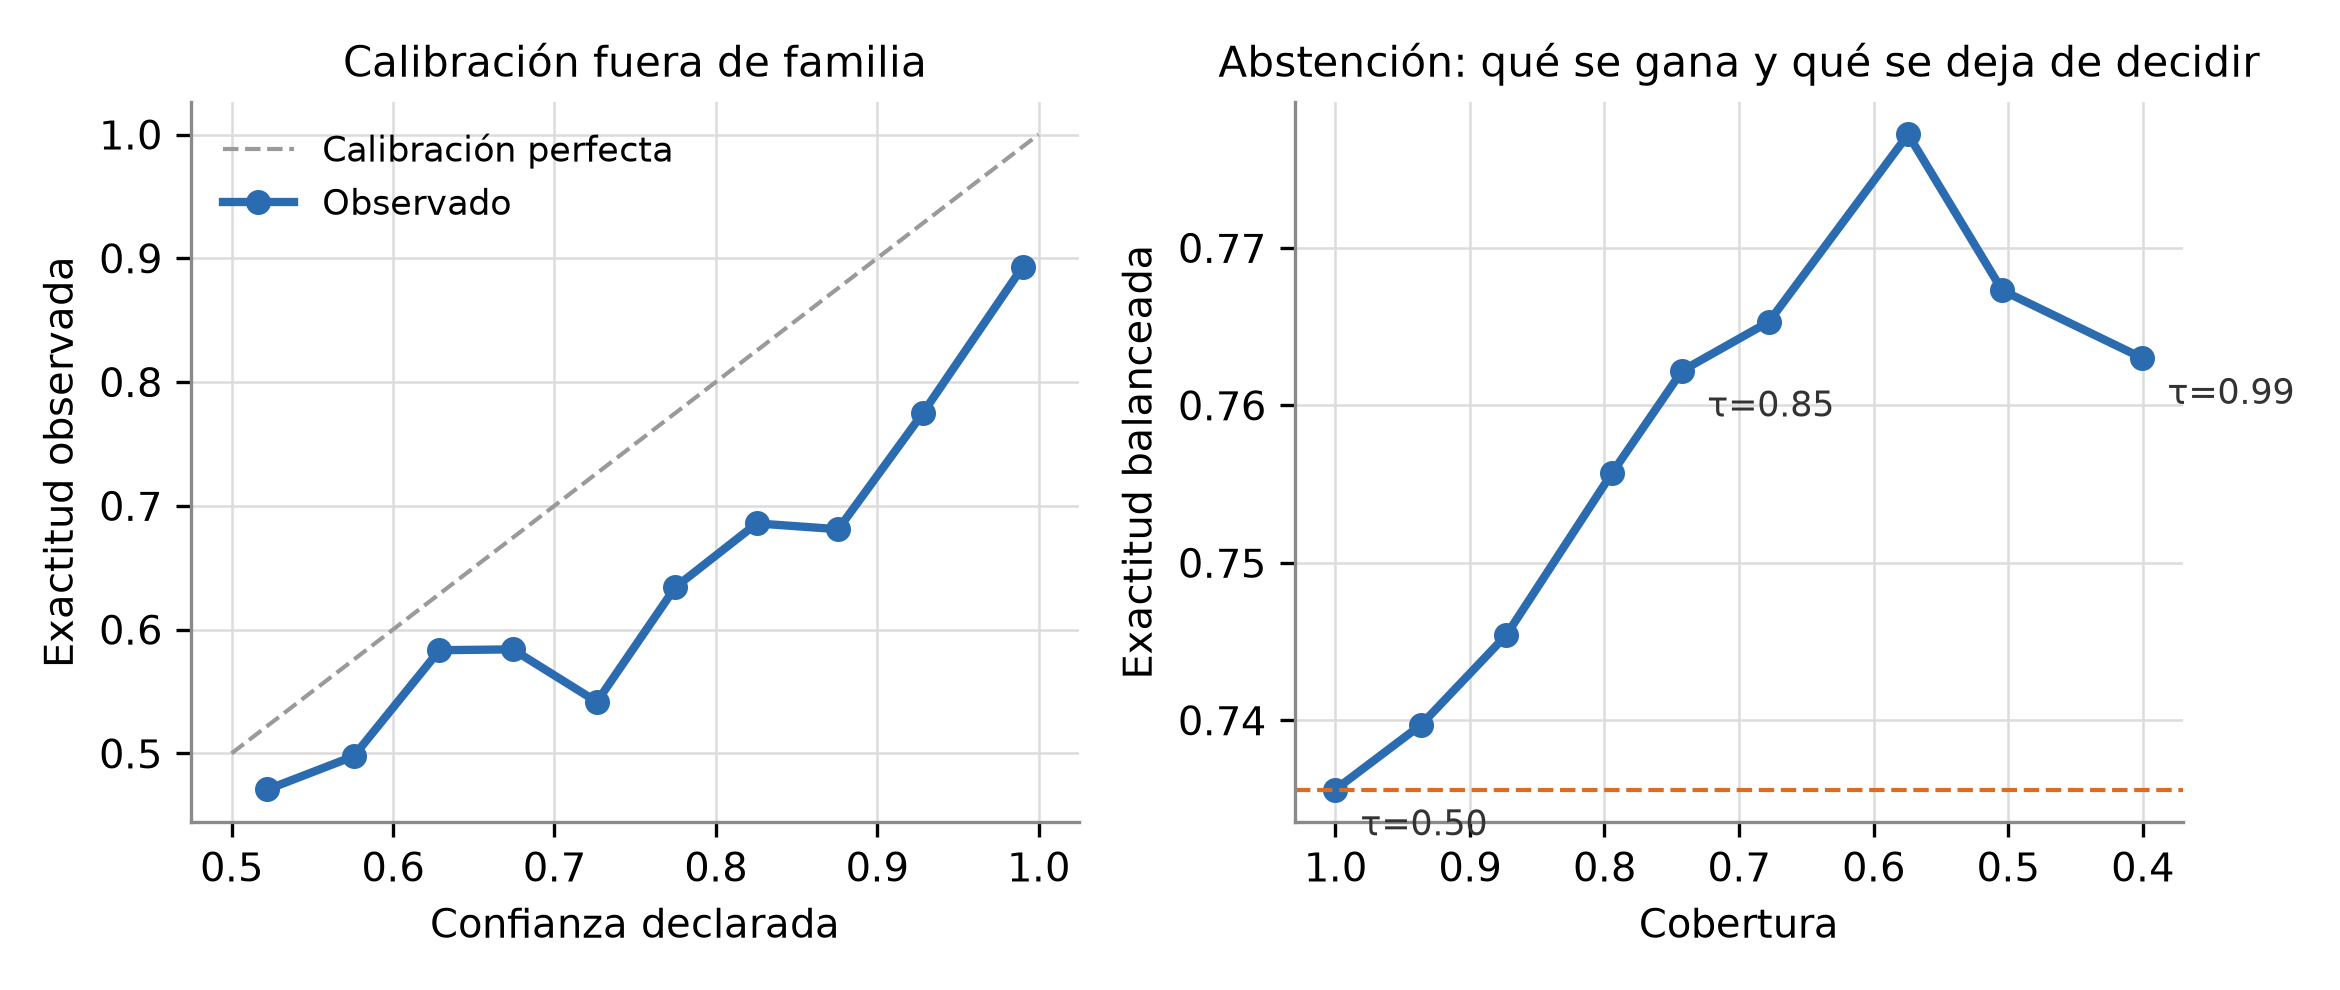
\includegraphics[width=0.96\textwidth]{figuras/fig_cpu_umbral_calibracion_20260919.png}
    \caption[Calibración y compromiso de la abstención en CPU]{A la izquierda, confianza declarada frente a exactitud observada sobre familias no vistas; la curva por debajo de la diagonal indica sobreconfianza. A la derecha, exactitud balanceada alcanzable en función de la cobertura al variar el umbral; ambas curvas usan una sola semilla de muestreo, por lo que sus valores difieren ligeramente de los promedios de cinco semillas de la Tabla \ref{tab:cpu-selectiva}. Fuente: elaboración propia.}
    \label{fig:cpu-umbral-calibracion}
\end{figure}

La salida \textit{revisar} activa una política conservadora: el sistema conserva la frecuencia vigente y espera dos intervalos \textit{uncore} válidos consecutivos antes de aceptar una caracterización física. En cuanto al costo, la inferencia de una fila toma 243~\textmu s de mediana y 404~\textmu s en el percentil 99 para XGBoost, frente a 450 y 475~\textmu s de la regresión logística y 5.3 y 5.5~ms de los bosques, medidos en paccaA100. Estas cifras incluyen la sobrecarga del intérprete de Python y son una cota superior para una implementación integrada en el agente.


\subsubsection{Dónde está el límite del resultado}
\label{sec:resultados-cpu-limite}

Cuatro resultados independientes indican que el límite proviene de la información contenida en los contadores y no del modelo.

El primero es que un clasificador sin ajuste, de 25 vecinos más cercanos sobre cuatro tasas estandarizadas, alcanza 0.684 con el mismo protocolo, y 0.699 si recibe además la frecuencia: queda a menos de 0.045 del modelo final. El segundo es la existencia de perfiles gemelos entre familias de clase opuesta (Figura \ref{fig:cpu-perfiles-gemelos}). El caso más simétrico enfrenta a \textit{gap\_pr}, \textit{memory-bound}, con la fase \textit{compute-bound} de \textit{phasic}: la primera tiene MPKI de 0.82, IPC de 1.11 y tasa de fallos de 0.76; la segunda, MPKI de 0.94, IPC de 0.97 y tasa de fallos de 0.72. El par más cercano en distancia estandarizada, sin embargo, es otro: la celda rara \textit{memory-bound} de \textit{rajaperf\_basic\_mat\_mat\_shared} (apenas el 0.1\% de sus intervalos; la familia es, en conjunto, \textit{compute-bound}) queda a la mitad de distancia de la celda \textit{compute-bound} típica de \textit{rajaperf\_basic\_pi\_reduce}, dos kernels de la misma suite. Ningún modelo que reciba solo esas señales puede separar estos pares, y las tres familias involucradas están entre las de peor resultado.

\begin{figure}[H]
    \centering
    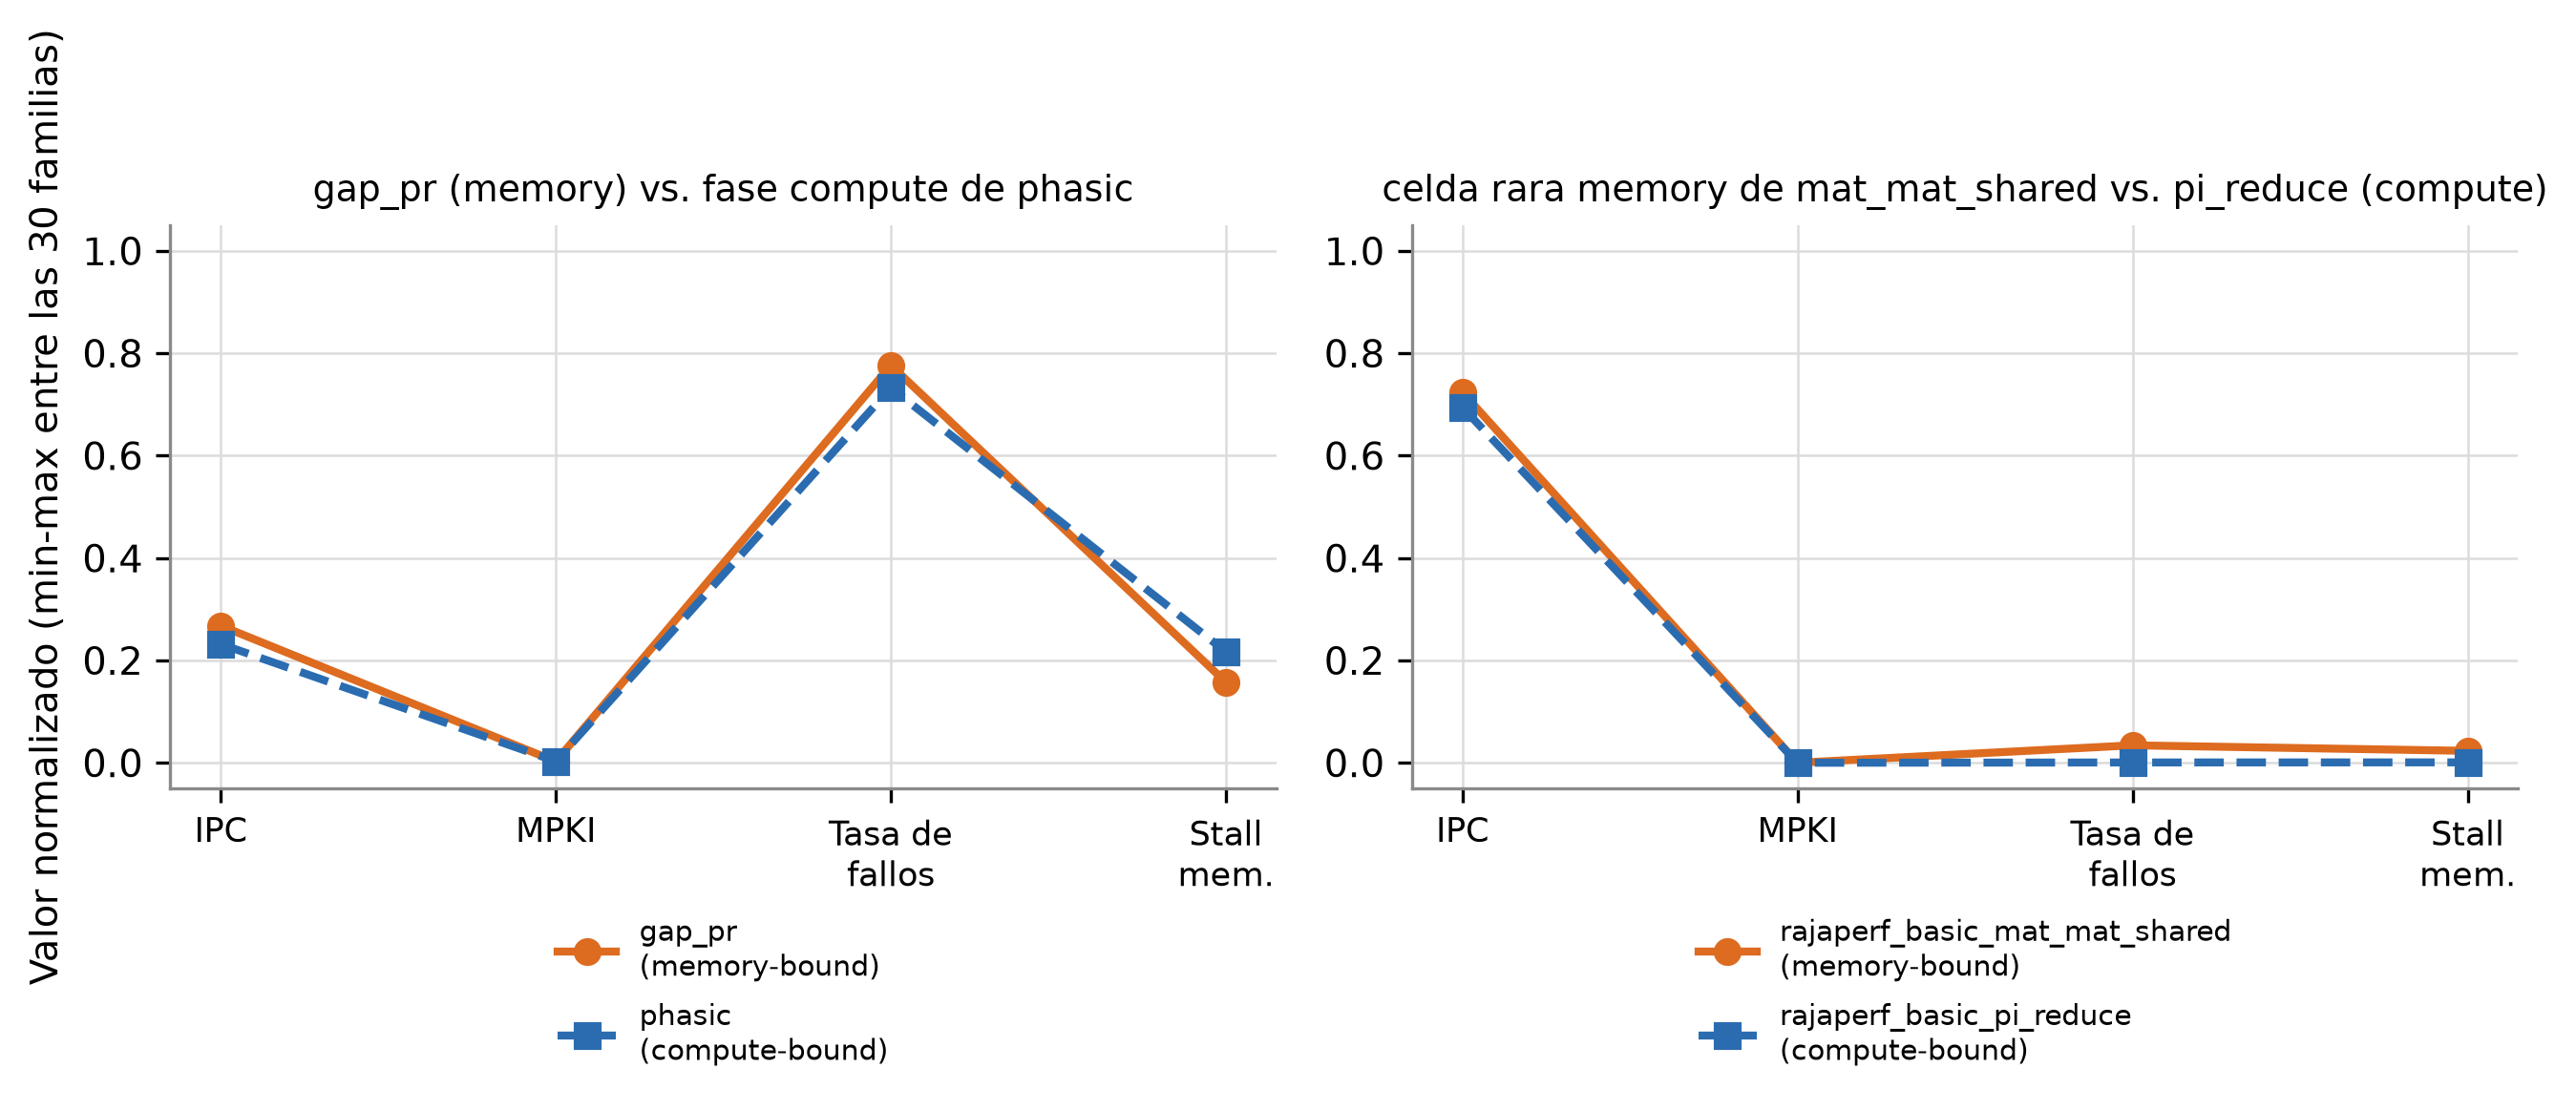
\includegraphics[width=0.96\textwidth]{figuras/fig_cpu_perfiles_gemelos_20260922.png}
    \caption[Perfiles de celdas confusables entre clases opuestas]{Cuatro variables de entrada, normalizadas al rango de las 30 familias, para los dos pares de celdas más confusables entre clases opuestas. Fuente: elaboración propia.}
    \label{fig:cpu-perfiles-gemelos}
\end{figure}

El tercero es la posición respecto del \textit{ridge} (Figura \ref{fig:cpu-margen-ridge}). Los intervalos situados a menos de un factor dos del punto de inflexión son el 12.5\% del total y se clasifican con 0.521 de exactitud, frente a 0.799 en el resto; concentran el 25.3\% de los errores. La ambigüedad cerca de la frontera explica una parte del error, pero tres cuartas partes de los fallos ocurren lejos del \textit{ridge}, donde la etiqueta no es ambigua. Ese error residual, además, no es simétrico alrededor de la frontera: en la franja inmediatamente \textit{compute-bound} (de 0 a 0.5 octavas por encima del \textit{ridge}) la exactitud es 0.318, mientras que en la franja simétrica del lado \textit{memory-bound} (de $-0.5$ a 0 octavas) es 0.766. El modelo no se equivoca por igual a ambos lados de la frontera: cerca de ella, empuja sistemáticamente hacia \textit{memory-bound}, lo mismo que ya se observa en el déficit de sensibilidad de \textit{compute-bound} frente a \textit{memory-bound} (sección \ref{sec:resultados-cpu-final}), y es consistente con los perfiles gemelos del párrafo anterior, en los que la fase \textit{compute-bound} de \textit{phasic} se confunde con \textit{memory-bound}.

\begin{figure}[H]
    \centering
    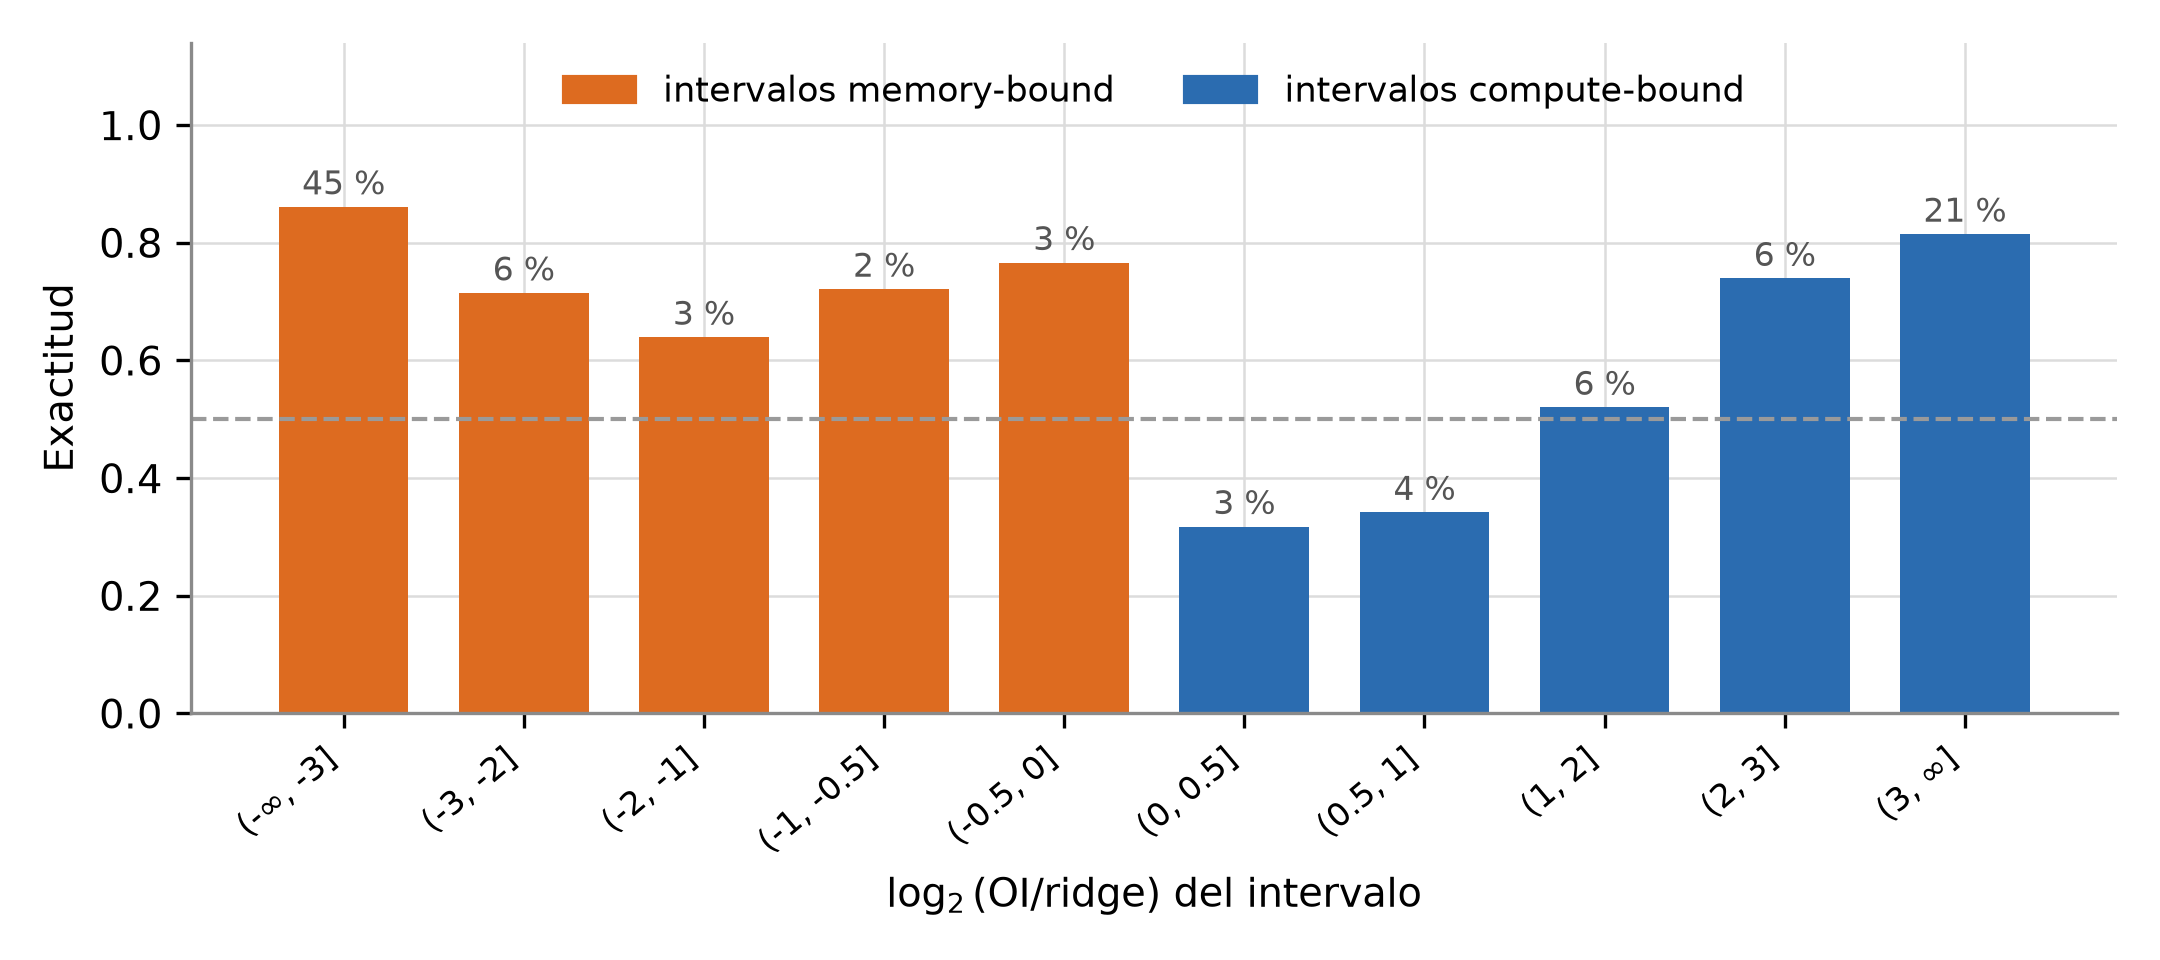
\includegraphics[width=0.94\textwidth]{figuras/fig_cpu_margen_ridge_20260919.png}
    \caption[Exactitud según la distancia al \textit{ridge}]{Exactitud del modelo final por franja de $\log_2(\mathrm{OI}/\mathrm{ridge})$. El porcentaje sobre cada barra indica qué fracción de los intervalos cae en esa franja. Las franjas negativas corresponden a intervalos \textit{memory-bound} y las positivas a \textit{compute-bound}. Fuente: elaboración propia.}
    \label{fig:cpu-margen-ridge}
\end{figure}

El cuarto es la curva de aprendizaje por número de familias (Figura \ref{fig:cpu-curva-aprendizaje}). Al ajustar con subconjuntos de 3 a 23 familias, el resultado sobre la familia retirada sube de 0.615 a 0.718, lo que implica aproximadamente 0.037 de ganancia cada vez que se duplica el catálogo. La diversidad algorítmica gobierna el resultado, y la mejora disponible por esa vía, dentro del alcance de este trabajo, es pequeña.

\begin{figure}[H]
    \centering
    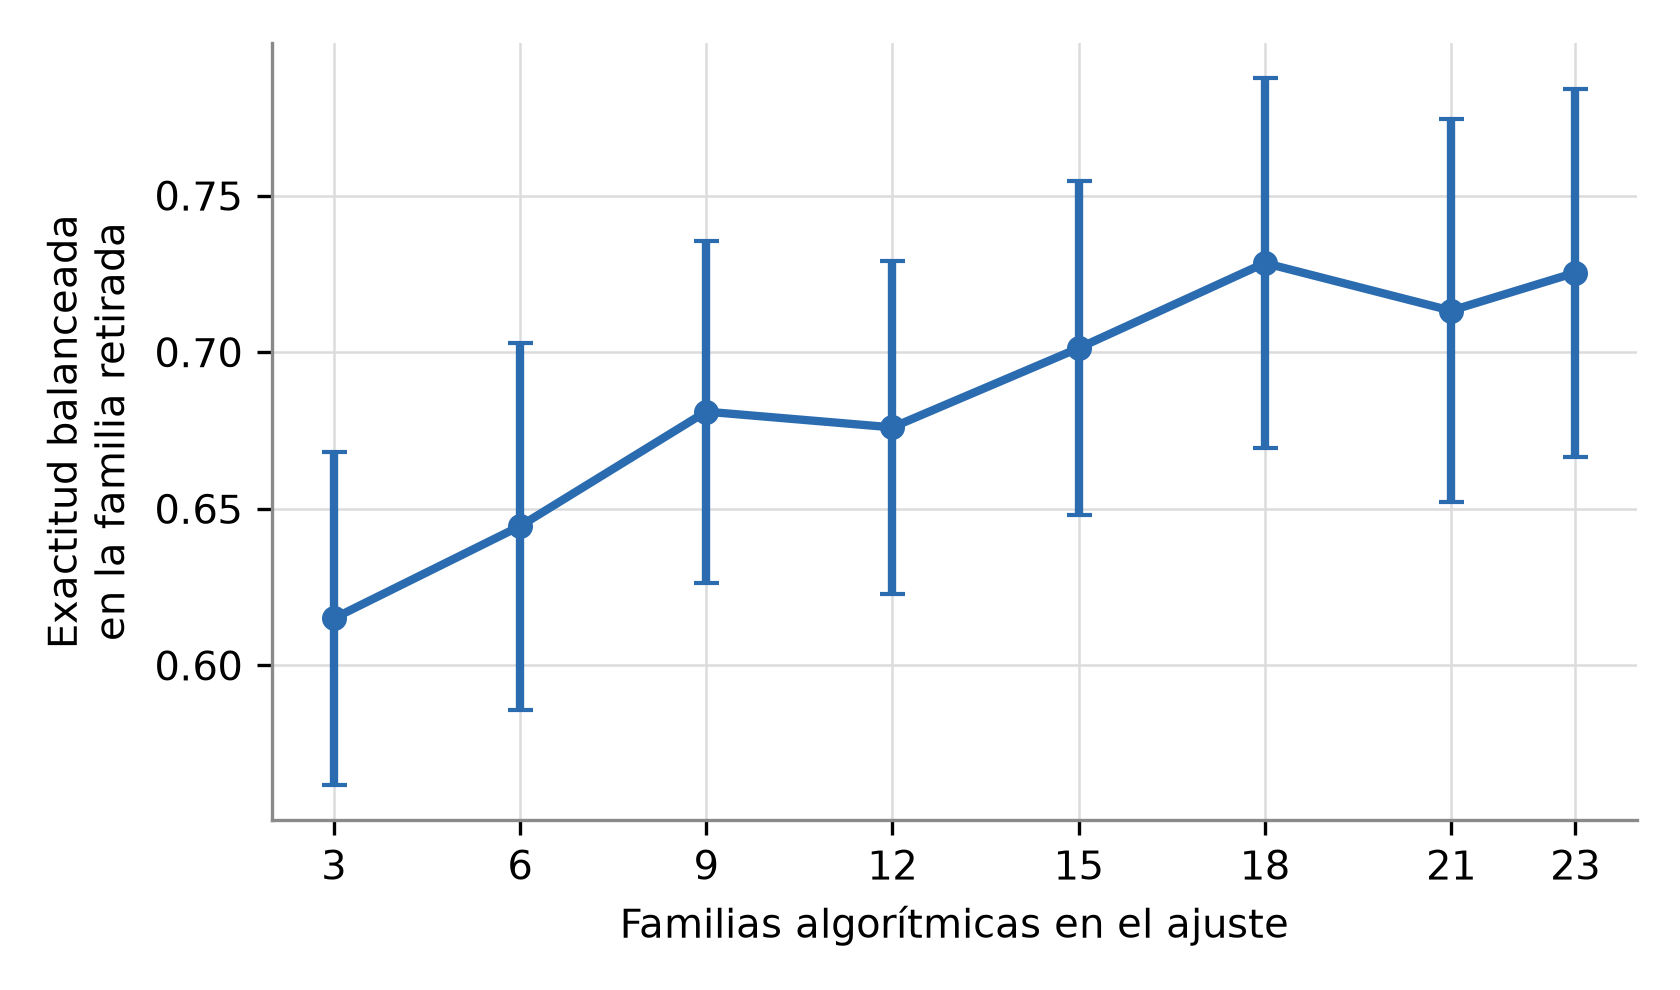
\includegraphics[width=0.72\textwidth]{figuras/fig_cpu_curva_aprendizaje_20260919.png}
    \caption[Curva de aprendizaje por número de familias]{Exactitud balanceada sobre la familia retirada en función del número de familias empleadas en el ajuste. Cada punto promedia las 30 familias retiradas y tres repeticiones de la selección; las barras indican el intervalo de confianza del 95\% entre familias. Fuente: elaboración propia.}
    \label{fig:cpu-curva-aprendizaje}
\end{figure}

Como referencia de límite superior, el mismo modelo con la intensidad operacional medida como entrada adicional alcanza 0.9989, frente a 0.728 sin ella. No es una mejora del modelo, porque la intensidad operacional es la cantidad con la que se define la etiqueta; por eso queda fuera del vector de entrada y solo muestra que la brecha entre 0.728 y 1 es información que los contadores de rendimiento no transportan.


\subsubsection{Síntesis del clasificador CPU}
\label{sec:resultados-cpu-sintesis}

El modelo es un XGBoost de 100 árboles y profundidad 6 que recibe seis variables derivadas de los contadores de rendimiento (cinco tasas normalizadas y la frecuencia observada), se ajusta dando el mismo peso total a cada combinación de familia y clase, y responde \textit{compute-bound}, \textit{memory-bound} o \textit{revisar} según su confianza supere o no 0.85. Ante un algoritmo que nunca vio clasifica correctamente el 72.8\% de los casos en la métrica balanceada por celda, cifra que sube a 73.8\% si se le permite abstenerse en el 27.8\% de los intervalos. La referencia sin capacidad de discriminar queda en 0.464 y la inferencia cuesta 404~\textmu s en el peor percentil medido.

Tres decisiones de diseño resultaron indiferentes: el algoritmo de aprendizaje, el tamaño del vector de entrada y los hiperparámetros. Elegir Random Forest en lugar de XGBoost, usar seis variables en lugar de doce o ajustar los hiperparámetros mueve el resultado menos de lo que lo mueve cambiar de conjunto de familias. Lo que gobierna el resultado es la diversidad del catálogo frente a la información de los contadores: la etiqueta se define por FLOPs sobre bytes de DRAM, mientras que el modelo observa fallos de caché, ciclos detenidos e instrucciones retiradas, que no guardan una relación fija con esa razón cuando cambia el algoritmo.

Quedan tres líneas de trabajo, fuera del alcance de esta fase. La primera es dar contenido a la salida \textit{revisar}: en lugar de solo esperar, el agente de la Fase 3 podría medir la etiqueta física de una fracción mínima de intervalos de la carga en ejecución; esa capacidad se diseña y evalúa allí, con su propio método y protocolo, y no se anticipa aquí con una cifra suelta. La segunda es ampliar el catálogo con familias elegidas por su distancia a los perfiles ya cubiertos y reservar algunas para una prueba externa sellada; las seis familias de cómputo denso de RAJAPerf provienen de una misma suite, de modo que su independencia entre sí es menor que la de familias de suites distintas. La tercera es medir la latencia dentro del agente y no en el intérprete.

Los datos, las figuras y las tablas de esta sección se reproducen con \path{fase2_clasificador/analysis/cpu_quality_report.py} y \path{docs/libro/scripts/generar_figuras_modelo_cpu.py}, sobre los artefactos de \path{docs/libro/datos/cpu_calidad_30fam}.

\subsection{Política de frecuencia por clase en CPU}
\label{sec:resultados-cpu-politica}

La política CPU compara la mediana de tres repeticiones por kernel y frecuencia con su propio REF. Un nivel debía mejorar el EDP agregado con evidencia estadística y al menos 1\% para adoptarse; ese mínimo se fijó después de ver el resultado y se declara como tal. Se excluyeron las variantes \textit{phasic}, cuyo trabajo cambia con la frecuencia pese a su duración fija. La Tabla \ref{tab:cpu-politica-ic} resume la decisión; la rejilla completa está en la Tabla \ref{tab:cpu-politica-detalle} del anexo.

La política resultante es \textit{no actuar} en ambas clases (Tabla \ref{tab:cpu-politica-ic} y Figura \ref{fig:cpu-politica-forest}). La Figura \ref{fig:cpu-energia-relativa} separa la energía y el tiempo que producen ese resultado. En cómputo, F0 mejora 0.56\% frente a REF, menos que el efecto mínimo relevante de 1\%; todos los niveles inferiores empeoran el EDP. En memoria tampoco hay ganancia agregada a menor reloj. Algunos kernels STREAM presentan ahorros puntuales entre 4 y 11\% en su mejor nivel, pero el signo y la magnitud varían entre niveles y repeticiones; no justifican una regla común.

\begin{table}[H]
\centering
\caption{Síntesis de la política CPU. Las ganancias son de EDP frente a REF; la rejilla completa se conserva en la Tabla \ref{tab:cpu-politica-detalle} del Anexo \ref{anexo:resultados-complementarios}.}
\label{tab:cpu-politica-ic}
\small
\begin{tabular}{@{}p{2.5cm}p{7.7cm}p{3.1cm}@{}}
\toprule
\textbf{Clase} & \textbf{Evidencia decisiva} & \textbf{Política} \\
\midrule
Cómputo & F0: $+0.56\%$ (IC95 $[0.27;1.38]$), por debajo del mínimo relevante de $1\%$; F1--F8 empeoran & No actuar \\
Memoria & F1: $-5.4\%$ (IC95 $[-6.8;-3.4]$); ningún nivel bajo mejora el agregado & No actuar \\
\bottomrule
\end{tabular}
\end{table}

\begin{figure}[H]
    \centering
    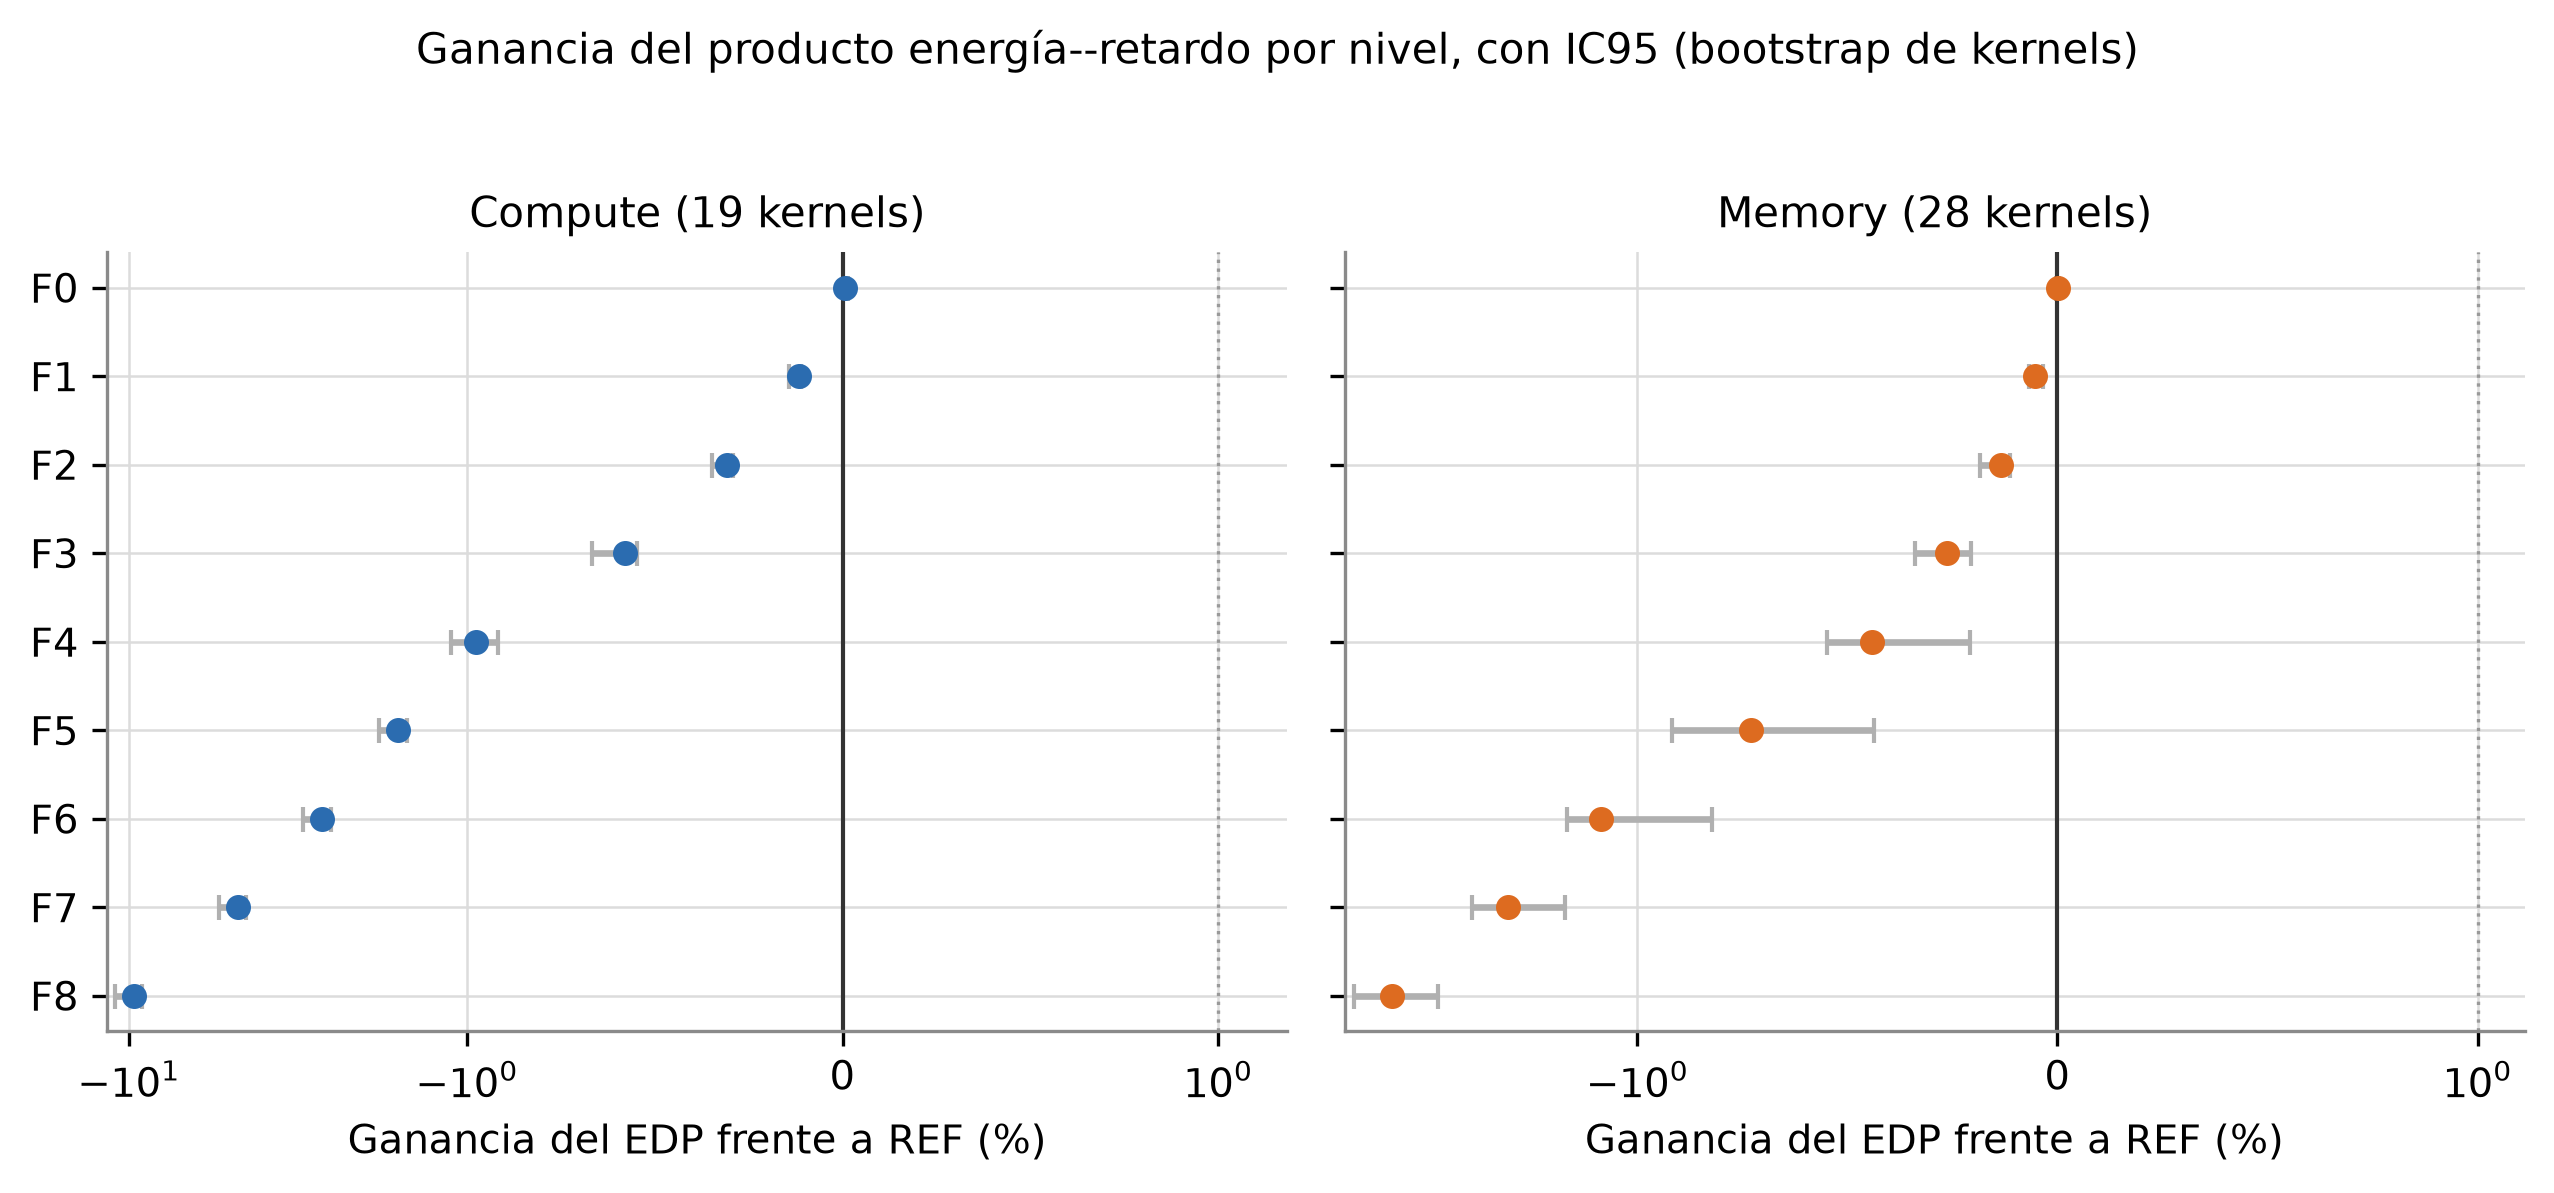
\includegraphics[width=0.85\textwidth]{figuras/fig_cpu_politica_forest_20260922.png}
    \caption[Ganancia del EDP por nivel y clase, en forma de \textit{forest plot}]{La rejilla completa de la Tabla \ref{tab:cpu-politica-detalle}, en forma gráfica. El eje horizontal es simétrico-logarítmico para mostrar a la vez F0, cercano a cero, y F8, con una pérdida de casi un orden de magnitud. Ningún nivel deja el intervalo de confianza por encima de cero de forma útil. Fuente: elaboración propia.}
    \label{fig:cpu-politica-forest}
\end{figure}

\begin{figure}[H]
    \centering
    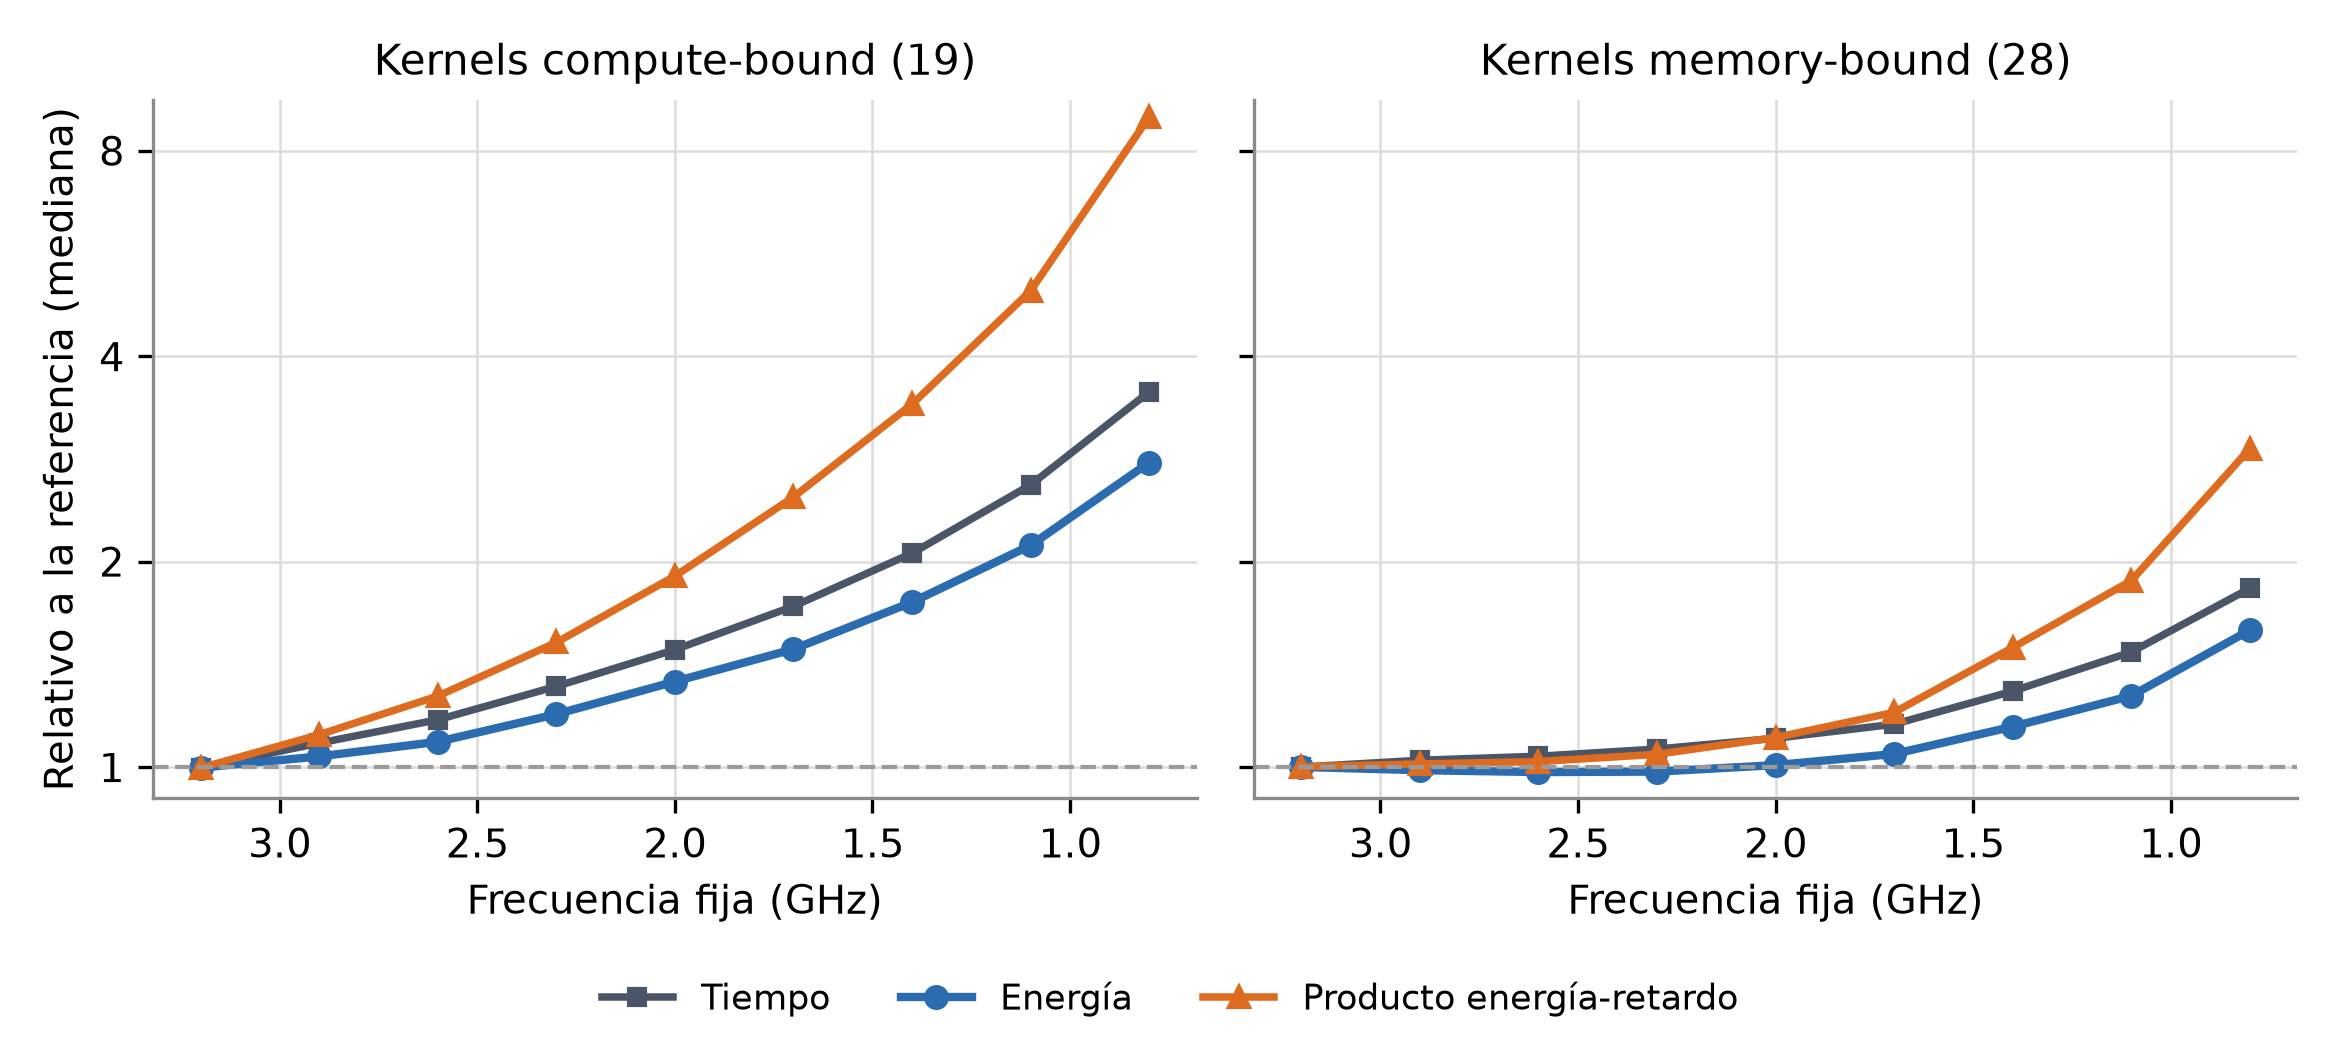
\includegraphics[width=0.94\textwidth]{figuras/fig_cpu_energia_relativa_20260920.png}
    \caption[Energía, tiempo y producto energía--retardo por nivel de frecuencia]{Mediana entre kernels de la energía (paquete y DRAM), el tiempo y el producto energía--retardo de cada nivel fijo, relativos a la referencia nativa, para las dos clases. El eje vertical es logarítmico. Fuente: elaboración propia.}
    \label{fig:cpu-energia-relativa}
\end{figure}

El intervalo de confianza \textit{bootstrap} y el valor $p$ de Wilcoxon de la Tabla \ref{tab:cpu-politica-detalle} responden preguntas distintas y pueden discrepar en apariencia: el primero remuestrea kernels para acotar la ganancia agregada, y el segundo prueba, kernel por kernel, si el signo de la diferencia frente a REF es consistente. Es el caso de F1 y F2 en memory, donde el IC95 excluye el cero pero $p$ no baja de 0.05: con solo 28 kernels y una ganancia heterogénea entre ellos, ambas lecturas son compatibles.

El mecanismo es un piso de potencia de unos 85~W, equivalente al 84\% de la potencia a 3.2~GHz (Figura \ref{fig:cpu-energia-piso}). Reducir la frecuencia a 0.8~GHz ahorra solo 15\% de potencia mientras alarga la ejecución. Incluso un oráculo que eligiera el mejor nivel medido por kernel ganaría 2.2\% en promedio; 22 de 47 kernels quedarían por debajo del efecto mínimo de 1\%. Esta cota es optimista porque el mejor nivel también captura ruido de medición.

\begin{figure}[H]
    \centering
    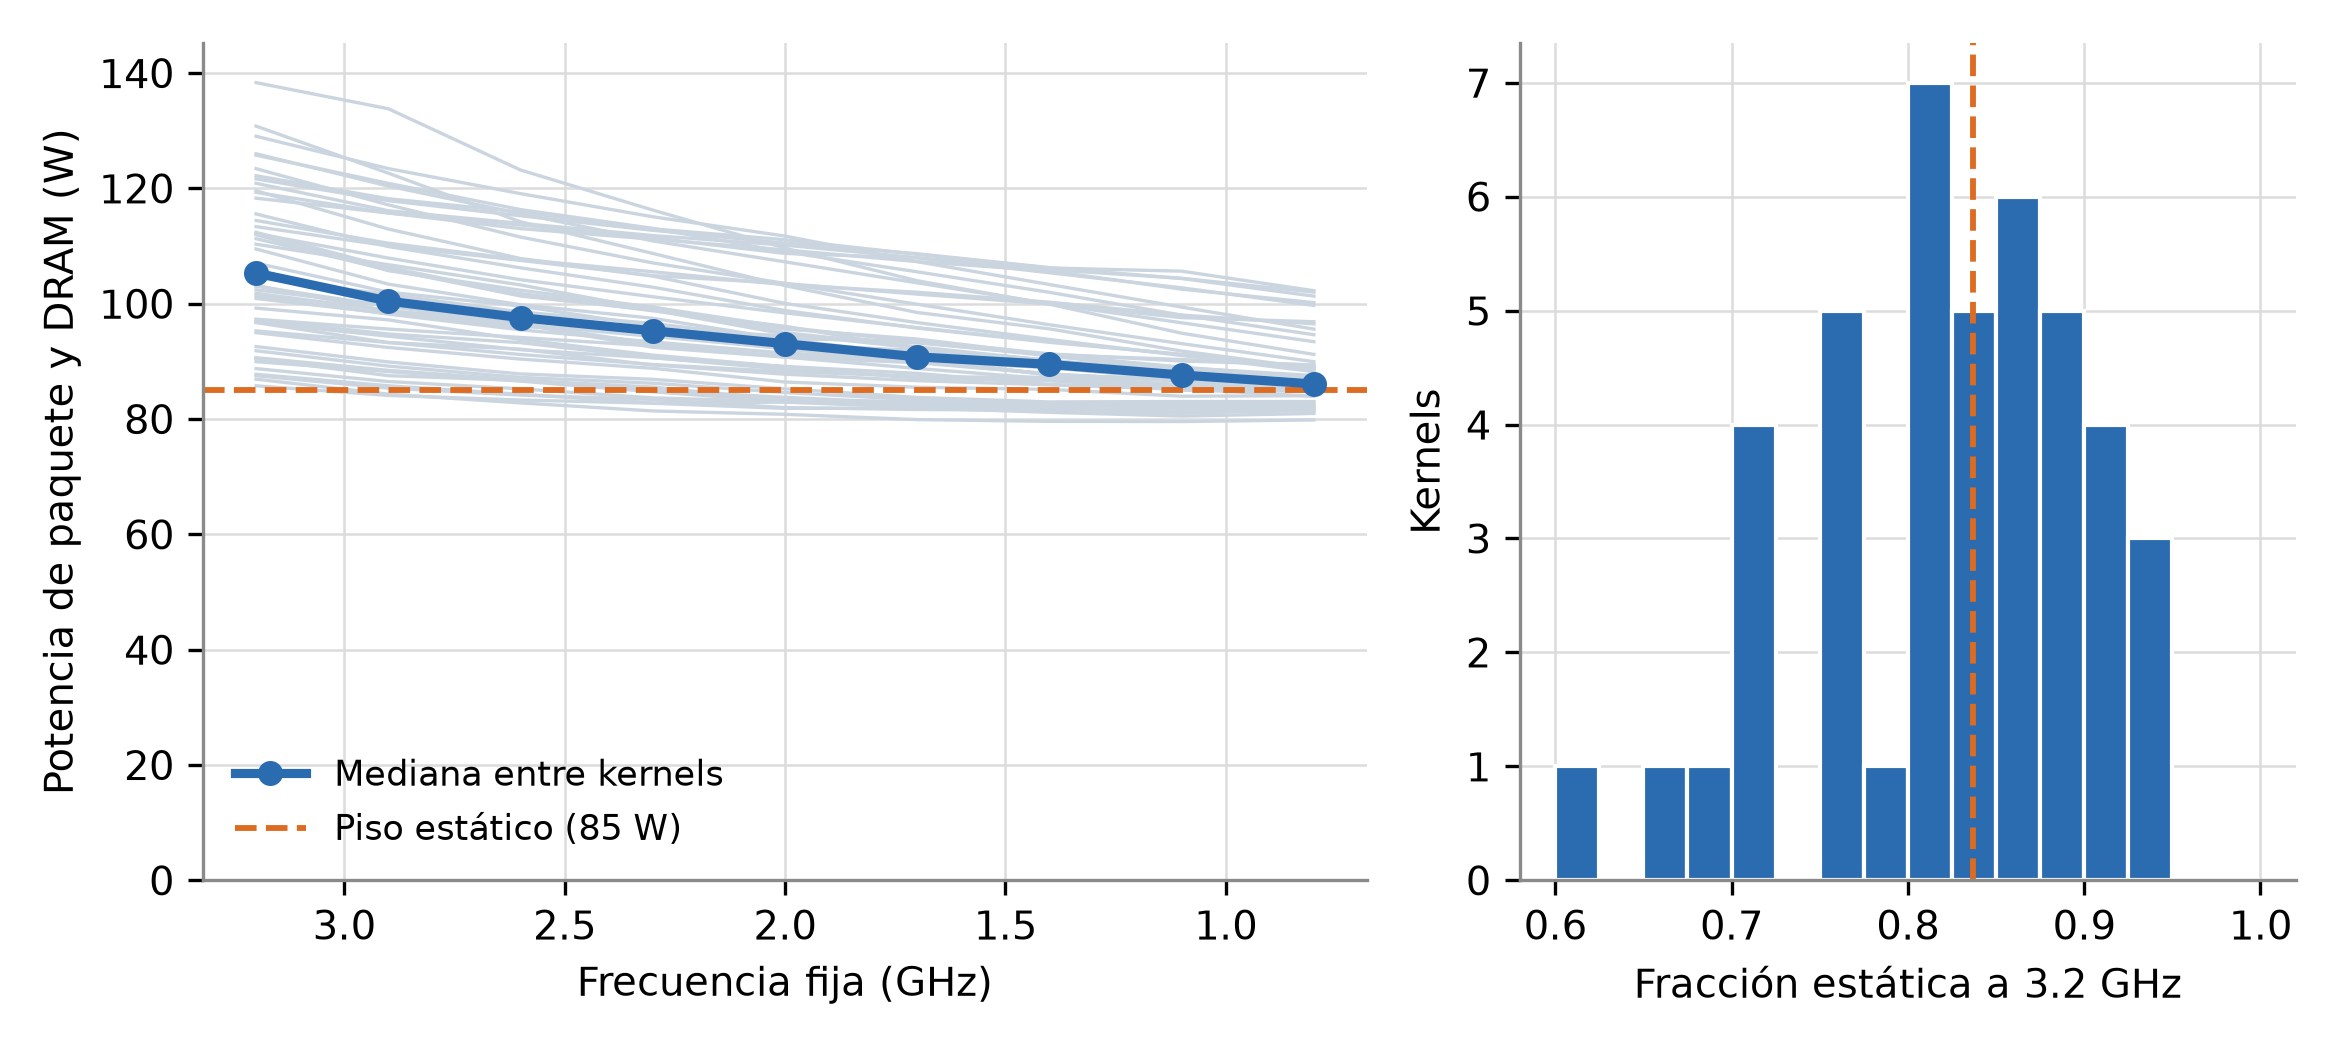
\includegraphics[width=0.94\textwidth]{figuras/fig_cpu_energia_piso_20260920.png}
    \caption[Potencia de paquete y DRAM frente a la frecuencia]{A la izquierda, potencia media de paquete y DRAM de cada kernel (líneas grises) y su mediana en cada nivel fijo, con el piso estático ajustado. A la derecha, distribución entre kernels de la fracción de la potencia a 3.2~GHz que corresponde al piso. Fuente: elaboración propia.}
    \label{fig:cpu-energia-piso}
\end{figure}

\subsubsection{Qué tamaño de efecto podía detectar este diseño}
\label{sec:resultados-cpu-potencia-diseno}

Un resultado de \textit{no actuar} solo es informativo si se acompaña del tamaño de efecto que el experimento podía distinguir, porque de lo contrario no separa la ausencia de efecto de la falta de sensibilidad. Tomando la familia algorítmica como unidad, que es la agrupación con la que se valida el clasificador, la desviación estándar del logaritmo del producto energía--retardo entre repeticiones de una misma combinación tiene mediana de 1.05\%, mientras que la dispersión entre las 19 familias \textit{memory\_bound} es de 5.35\% en F1 y 9.70\% en F2. Es decir, la varianza que limita la conclusión es heterogeneidad física entre cargas, entre cinco y diez veces mayor que el error de medición; aumentar el número de repeticiones no la habría reducido de forma apreciable.

De esas dispersiones se sigue el efecto mínimo detectable con potencia de 80\%: 1.75\% en F0, 3.38\% en F1, 6.05\% en F2 y 9.5\% en F3. La lectura correcta del resultado es, entonces, que con este catálogo quedan descartadas mejoras uniformes superiores a 3.4\% en F1, y que una mejora del orden del 1\%, el efecto mínimo relevante declarado, es indetectable por construcción con 19 familias. Esto acota el resultado en lugar de dejarlo abierto, y es consistente con el piso de potencia descrito arriba: el margen físico disponible es menor que la resolución que el diseño puede ofrecer.

Dado que la clase agregada mezcla cargas con respuestas de signo opuesto, se evaluó además si una regla más fina, condicionada a una variable del vector de entrada, permitía actuar sobre una subpoblación. La regla se congeló antes de medir y se probó en familias nuevas, ajenas a las 30 de entrenamiento, en dos pruebas externas independientes; ambas quedaron refutadas según los criterios declarados de antemano. El detalle queda registrado junto a la tabla de política en \texttt{policy\_cpu.json}. La conclusión operativa de la fase es, por tanto, \textit{no actuar} en ambas clases, sustentada en el piso de potencia medido y no en la ausencia de intentos de refinamiento.

\subsection{Invarianza del clasificador de CPU frente a la acción del agente}
\label{sec:resultados-cpu-frecuencia-contrafactual}

La frecuencia observada es una de las seis variables del clasificador de CPU y el agente la modifica, de modo que se aplicó la misma auditoría contrafactual de la GPU. Sobre el modelo final y sus 1.31 millones de intervalos de 49 kernels, forzar la frecuencia a un valor fijo cambia entre 4 y 11\% de las predicciones (Tabla \ref{tab:cpu-contrafactual-frecuencia}), de modo que existe una dependencia moderada. Pero el cambio que el agente ejecuta es acotado, de F0 (3.2~GHz) a F1 (2.9~GHz): sobre las 179\,774 filas observadas cerca de 3.2~GHz solo cambia el 0.42\% de las predicciones. Con ese espacio de acción la retroalimentación por esta variable es despreciable, y el modelo de CPU se despliega sin modificaciones.



\section{Resultados de GPU}
\label{sec:resultados-gpu}

\subsection{Validación de control y etiquetado}
\label{sec:resultados-gpu-dvfs}
\label{sec:resultados-precision-gpu}

El actuador de GPU sostuvo el bloqueo del reloj de \textit{streaming multiprocessors} bajo carga. Las pruebas con objetivos de 600 y 1200~MHz registraron, respectivamente, 305 y 174 lecturas activas coincidentes con el valor solicitado. La restauración de frecuencia se verificó al finalizar las campañas dedicadas.

La etiqueta Roofline se construyó con la precisión observada mediante Nsight Compute. Este control excluyó kernels con precisión mixta cuya intensidad operacional no admite comparación con un único techo y evitó atribuir a los contadores convencionales el trabajo ejecutado por Tensor Cores. En el nivel de referencia, los puntos de inflexión medidos fueron 14.965852~FLOP/byte para FP32 y 6.898377~FLOP/byte para FP64.

\subsection{Diagnóstico del primer conjunto GPU}
\label{sec:resultados-gpu-dataset-final}
\label{sec:resultados-gpu-separabilidad}

La primera campaña GPU reunió 540 corridas planificadas para 18 kernels. Después de calibrar el warmup, 334 corridas de 16 kernels y 11 familias quedaron disponibles para el diagnóstico inicial. El conjunto estaba desbalanceado (Figura \ref{fig:gpu-balance-clases-final}), con 73 corridas \textit{compute\_bound} y 261 \textit{memory\_bound}, y la mayoría de las familias era homogénea respecto de su etiqueta.

El árbol de profundidad 1 obtuvo un F1 macro de 0.617 bajo validación \textit{leave-one-familia-out}, frente a 0.553 del clasificador mayoritario. Este valor no se adopta como resultado final. La evaluación mostró que, al retirar familias completas, muchos pliegues quedaban sin ejemplos de una clase. Además, la utilización de SM no separó de forma universal los dos regímenes. \textit{rodinia\_gaussian}, por ejemplo, fue \textit{memory\_bound} según Roofline, pero alcanzó utilizaciones de SM suficientemente altas para que el modelo lo confundiera con una carga \textit{compute\_bound}.

La evidencia no indicó que bastara ajustar el modelo sobre el mismo conjunto. Mostró que faltaban familias \textit{compute\_bound} variadas y alejadas del punto de inflexión. Por esta razón se cambió la estrategia desde la búsqueda de hiperparámetros hacia la ampliación experimental del catálogo y la revisión del protocolo de validación.

\begin{figure}[H]
    \centering
    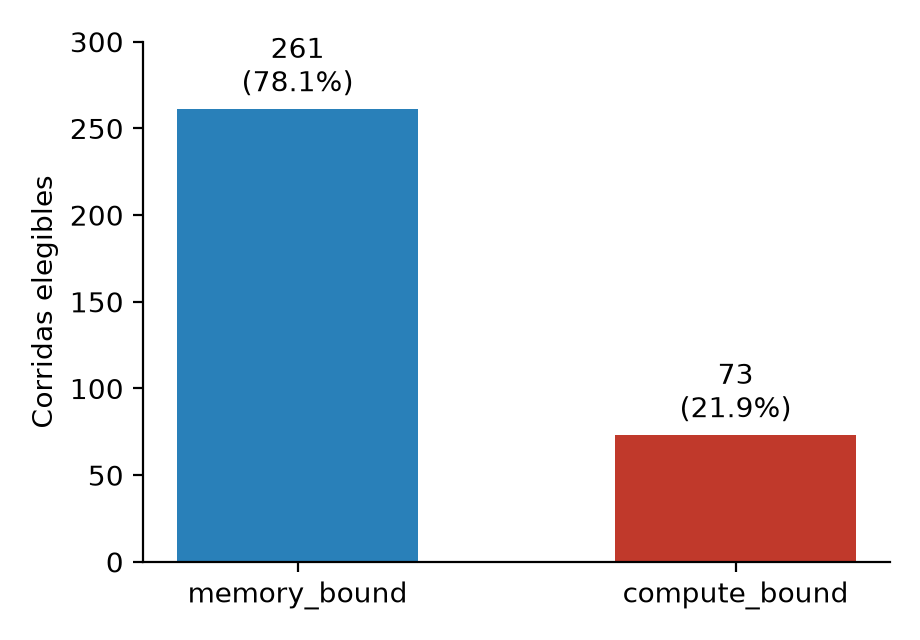
\includegraphics[width=0.5\textwidth]
        {figuras/fig_gpu_balance_clases_final_20260915.png}
    \caption[Balance de clases del conjunto GPU inicial]{Distribución de las 334 corridas elegibles del conjunto GPU empleado en el diagnóstico exploratorio. Fuente: elaboración propia.}
    \label{fig:gpu-balance-clases-final}
\end{figure}

\subsection{Reanálisis de campañas históricas con NVML}
\label{sec:resultados-gpu-oi-ventana}
\label{sec:resultados-gpu-gemm-evolucion}

El bloqueo de la nueva campaña multi-frecuencia impidió incorporar observaciones nuevas durante buena parte de esta fase. Se reanalizaron entonces campañas ya aceptadas, cuya etiqueta Roofline fue construida fuera de línea con \texttt{ncu} y cuya inferencia potencial dependía exclusivamente de NVML. El posproceso comparó esa intensidad con el \textit{ridge} correspondiente a la frecuencia y precisión de cada corrida, y difundió la misma etiqueta a todas sus lecturas NVML. No se registraron eventos CUPTI de lanzamiento en estas campañas, así que cada corrida se transformó en una sola observación mediante agregados robustos, sin duplicar ni sintetizar observaciones.

Un primer diagnóstico sobre esta representación mostró separación parcial entre clases (Figura \ref{fig:gpu-separabilidad-nvml}): la proyección PCA conserva la estructura global y t-SNE aproxima los vecindarios locales de ocho variables estáticas (mediana e IQR de utilización GPU, utilización de memoria, potencia y reloj SM). Ambas vistas contienen regiones dominadas por una clase, pero también regiones con etiquetas mezcladas. La separación por clase, calculada en el espacio original estandarizado, tuvo un coeficiente de silueta de 0.092, que describe separación débil. Un clasificador de tres vecinos que nunca observa ejemplos de la familia evaluada alcanzó F1 macro de 0.616, coherente con una señal transferible parcial: existe información física real en los agregados NVML, pero no una frontera estable para todas las familias.

\begin{figure}[H]
    \centering
    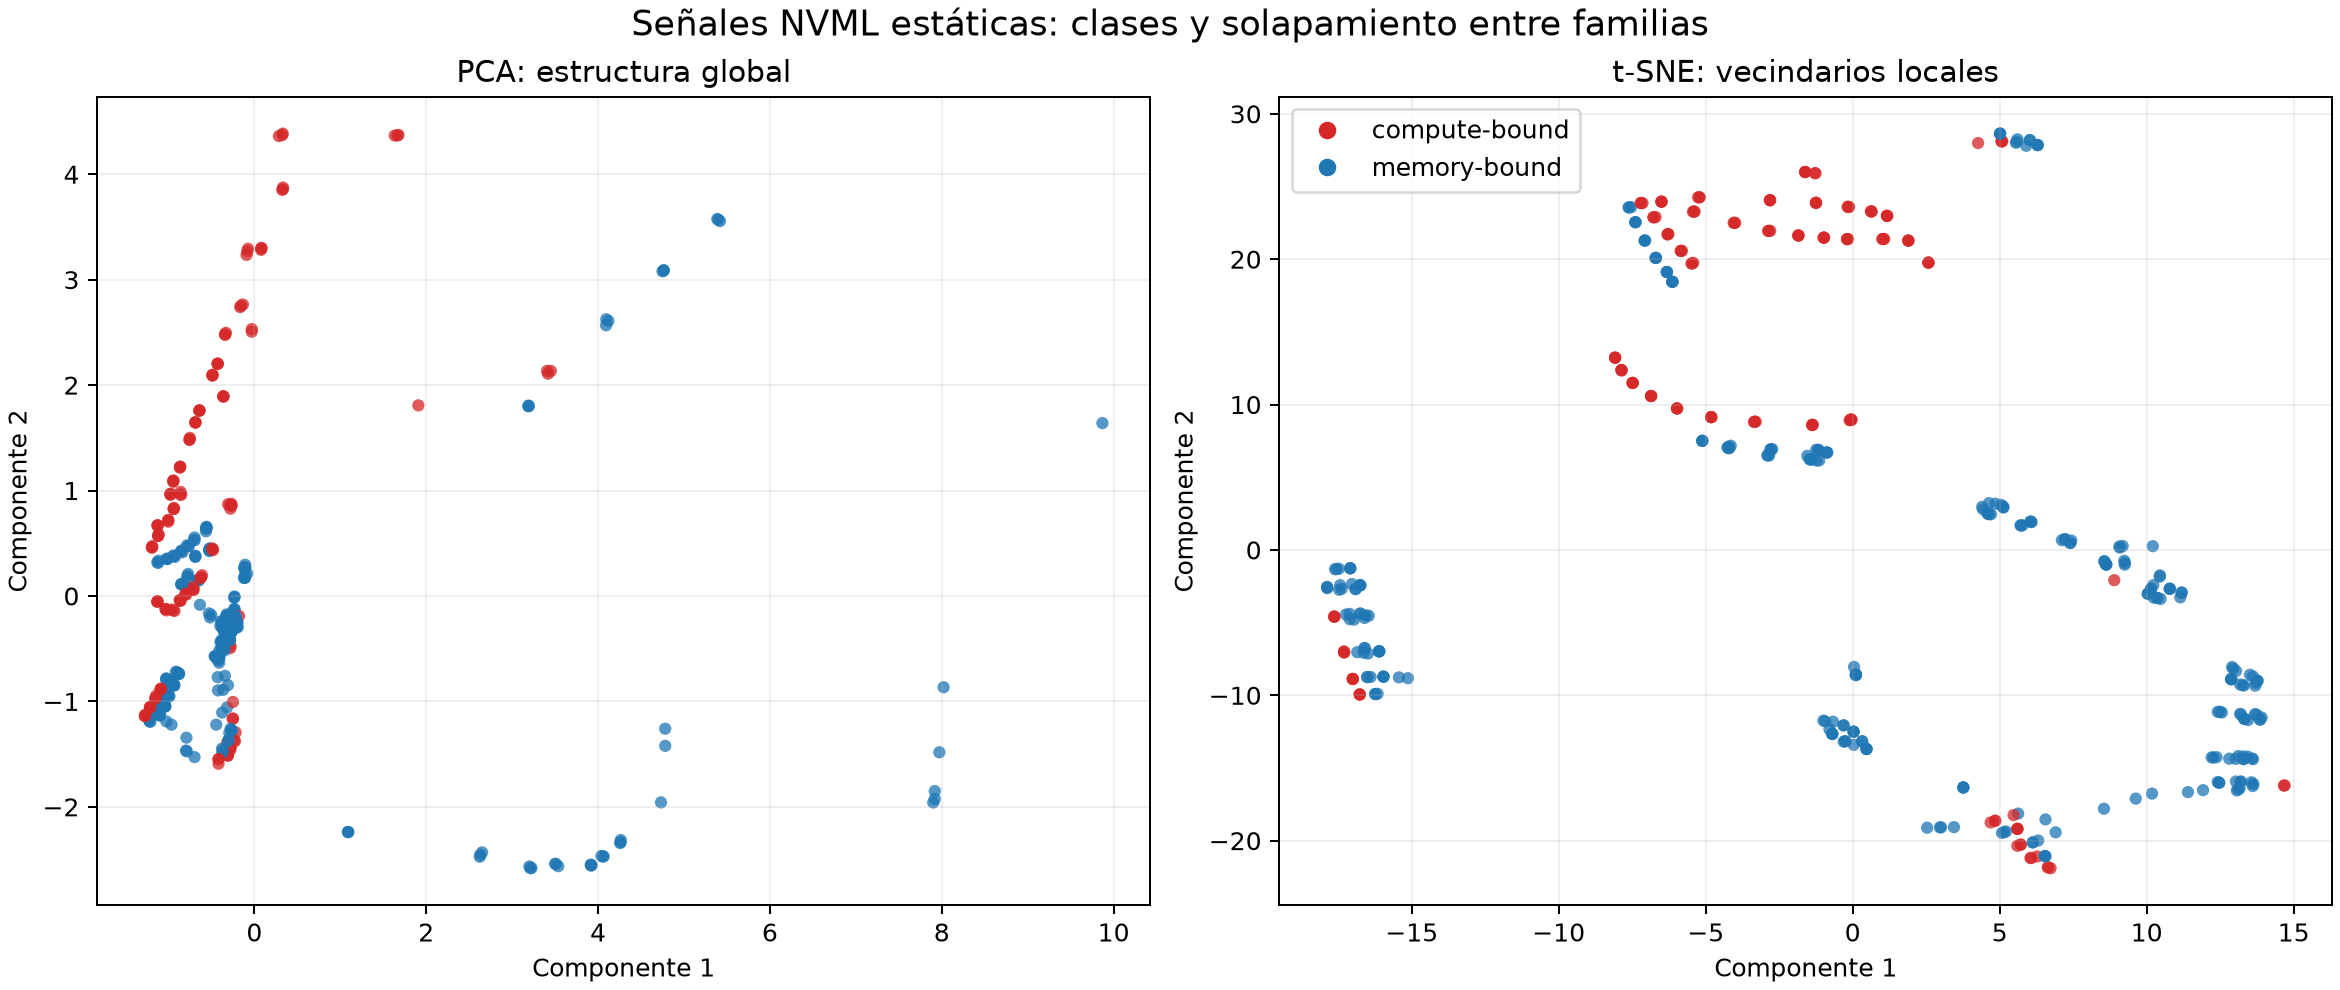
\includegraphics[width=\textwidth]
        {figuras/fig_gpu_separabilidad_nvml_20260918.png}
    \caption[Separabilidad de las clases GPU con señales NVML]{Proyecciones PCA y t-SNE de las medianas e IQR de utilización GPU, utilización de memoria, potencia y reloj SM. La proyección t-SNE es diagnóstica y no se utiliza para medir generalización. Fuente: elaboración propia.}
    \label{fig:gpu-separabilidad-nvml}
\end{figure}

A partir de ese diagnóstico se amplió el conjunto fusionando las campañas modernas aceptadas con tres campañas adicionales ya cerradas (\textit{kmeans}, miniBUDE y \textit{conv2d}), y se admitieron corridas que el gate de calidad había descartado únicamente por tener una fracción de muestras NVML posteriores al arranque menor al 50\%, cuando el conteo absoluto de muestras seguía siendo alto (cientos a miles por corrida). El conjunto resultante tiene 483 corridas y 16 familias algorítmicas, separando además los tres núcleos CUDA de RAJAPerf (GEMM, \textit{stencil} de calor y Jacobi 2D) que antes compartían una sola familia pese a tener perfiles Roofline distintos entre sí. La composición es de 171 corridas \textit{compute\_bound} y 312 \textit{memory\_bound}, trece de las dieciséis familias homogéneas respecto de su etiqueta.

La métrica de evaluación pasó a ser la exactitud balanceada sobre celdas familia por clase, el promedio del \textit{recall} de cada combinación observada. Esta métrica está bien definida incluso en familias de una sola clase y no depende de la prevalencia relativa de cada familia, a diferencia del F1 macro agrupado por volumen. La validación usó \textit{leave-one-familia-out}, cinco semillas de muestreo y un intervalo de confianza del 95\% por remuestreo \textit{bootstrap} de familias (2000 réplicas). Se compararon siete modelos candidatos con hiperparámetros fijos (Tabla \ref{tab:gpu-modelos-2026-09-22} y Figura \ref{fig:gpu-comparacion-modelos}): ninguno domina de forma concluyente. \textit{Random forest} (0.807), \textit{extra trees} (0.806) y la regresión logística (0.792) resultaron estadísticamente indistinguibles entre sí por remuestreo pareado de familias (probabilidad de superioridad entre 0.53 y 0.60), aunque \textit{random forest} sí superó con evidencia razonable a XGBoost (probabilidad de superioridad 0.961).

\begin{figure}[H]
    \centering
    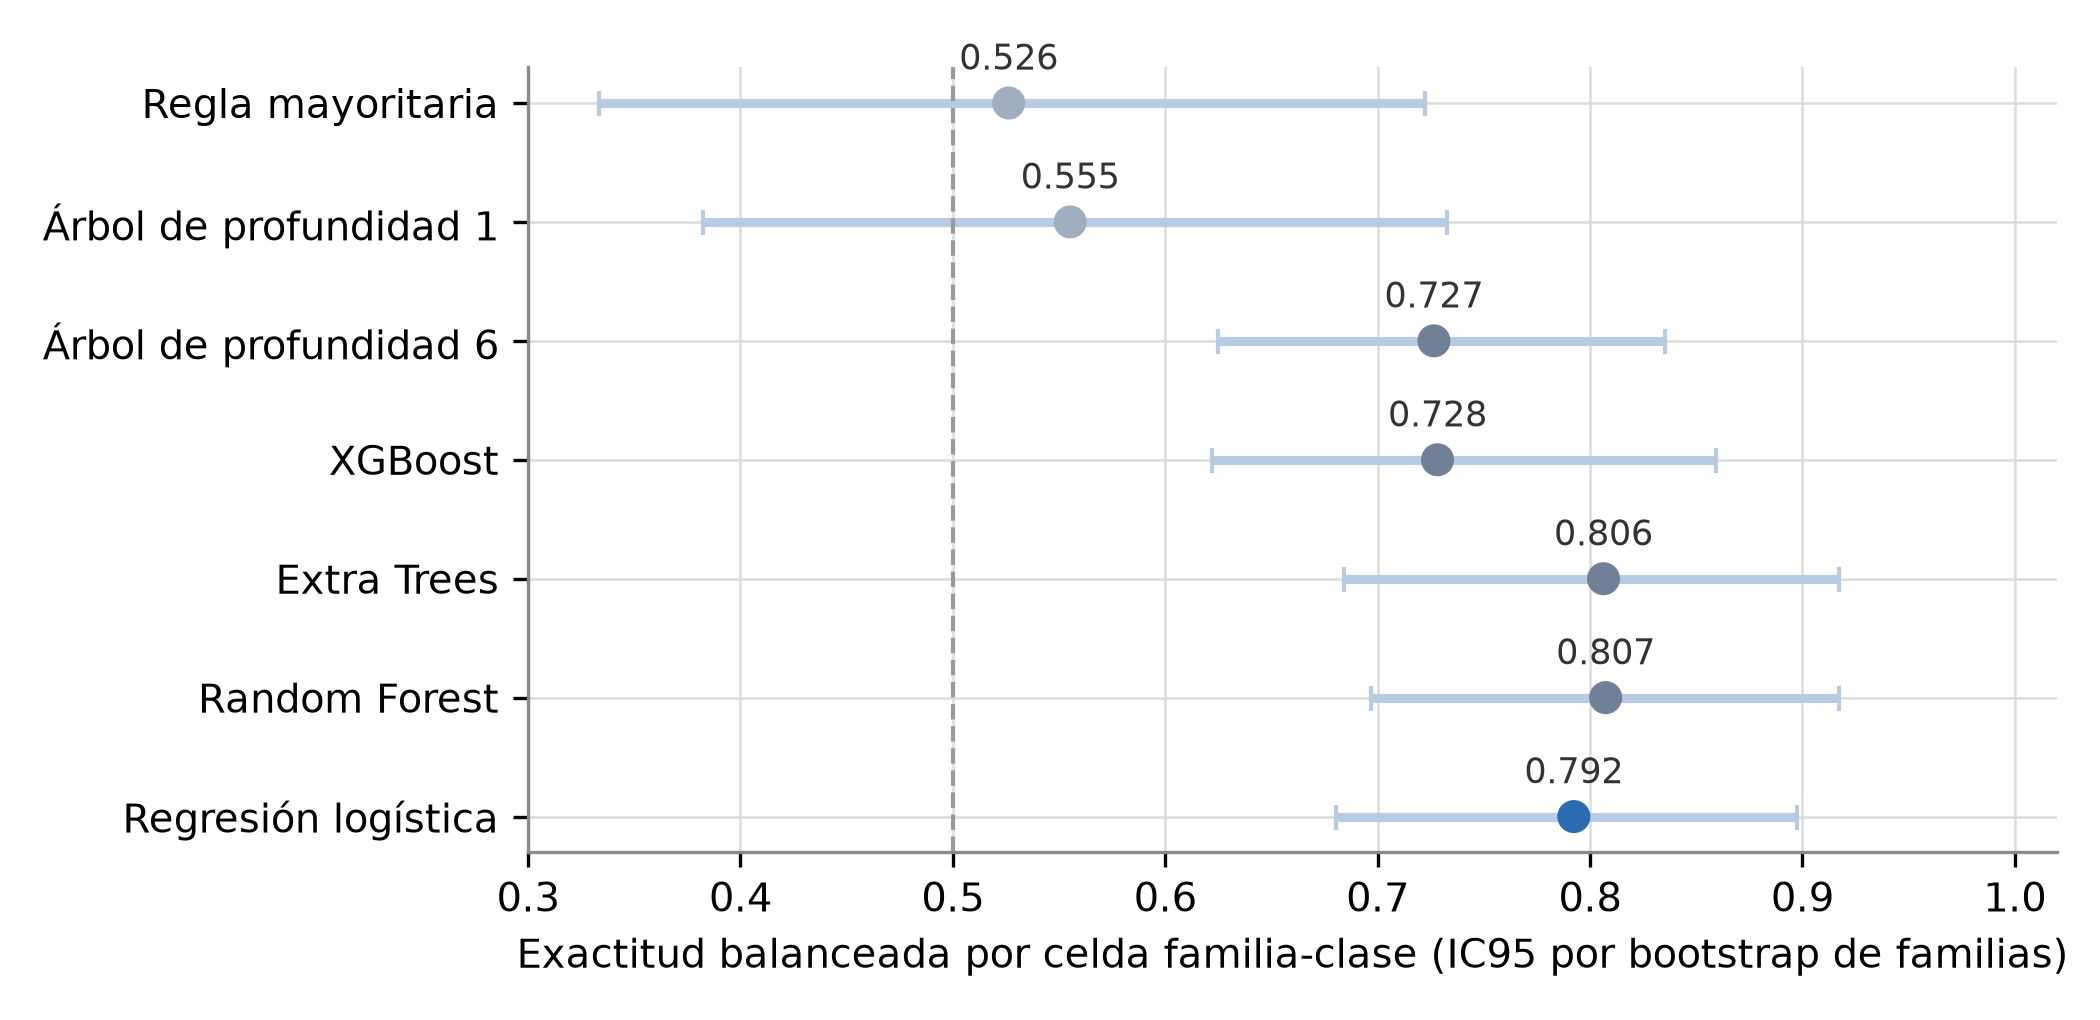
\includegraphics[width=\textwidth]{figuras/fig_gpu_comparacion_modelos_20260922.png}
    \caption[Comparación de modelos candidatos GPU]{Exactitud balanceada por celda familia-clase de los siete modelos candidatos, con intervalo de confianza del 95\% por \textit{bootstrap} de familias. Fuente: elaboración propia.}
    \label{fig:gpu-comparacion-modelos}
\end{figure}



Las cinco variables del conjunto candidato (Tabla \ref{tab:gpu-vif}) no presentan colinealidad relevante: el factor de inflación de varianza (VIF) máximo fue 2.26, muy por debajo del umbral convencional de 5 que suele usarse como señal de alerta.



Una búsqueda anidada de hiperparámetros con muestreador TPE (\textit{Optuna}), quince pruebas por modelo dentro de un \textit{leave-one-familia-out} interno, empeoró el resultado en cuatro de los cinco modelos ajustables respecto de la configuración fija (regresión logística de 0.792 a 0.767, \textit{random forest} de 0.807 a 0.778, \textit{extra trees} de 0.806 a 0.748, XGBoost de 0.740 a 0.724; solo el árbol de profundidad 6 mejoró, de 0.727 a 0.783). El mismo mecanismo documentado para el clasificador de fase de CPU explica esta caída: con familias limitadas, el criterio interno que Optuna maximiza no discrimina de forma confiable la configuración que generaliza mejor. La búsqueda de hiperparámetros se descarta para el candidato GPU por la misma razón que para CPU.

Con el empate entre \textit{random forest}, \textit{extra trees} y regresión logística ya establecido, el criterio de desempate para la referencia estática fue la latencia de inferencia de una sola fila, medida en \texttt{paccaA100}, el nodo de destino real. La regresión logística respondió en 400.9, 413.8 y 466.9 microsegundos (percentiles 50, 95 y 99); \textit{random forest} y \textit{extra trees} tardaron entre diez y doce veces más (percentil 99 de 5512.2 y 4989.9 microsegundos, respectivamente). La regresión logística usa las cuatro señales NVML, utilización GPU, utilización de memoria, potencia y reloj SM, todas por mediana, más la desviación estándar intracorrida de la utilización de memoria como quinta variable. Esta última se incorporó porque las medianas por sí solas diluyen el efecto de cargas con lanzamientos cortos y repetidos, como \textit{kmeans}, cuya intensidad operacional real es alta pero cuya firma NVML agregada se asemeja a una carga poco ocupada.

Dos familias no se resuelven con ninguna de las variables disponibles por una razón física, no por una limitación del modelo: el núcleo GEMM de RAJAPerf y \textit{LUD} de Rodinia cambian de régimen Roofline según el nivel de frecuencia de la corrida, porque el punto de inflexión se desplaza con el reloj mientras la intensidad operacional de cada kernel permanece fija. \textit{LUD}, por ejemplo, resultó \textit{memory\_bound} en los niveles de reloj más altos y \textit{compute\_bound} en los más bajos de la misma familia. Distinguir ese cambio exigiría una variable de distancia al \textit{ridge}, que constituye fuga de la propia etiqueta y por tanto no es admisible como entrada del clasificador.

La Figura \ref{fig:gpu-resultado-por-familia} desagrega el desempeño de la regresión logística estática por familia. El resultado no es parejo: ocho de las dieciséis familias superan 0.90 de exactitud, mientras \textit{dual\_cholesky} (0.23), el núcleo GEMM de RAJAPerf (0.50, la familia con cruce de \textit{ridge} ya descrita) y \textit{rodinia\_gaussian} (0.53, la familia más cercana al \textit{ridge} del catálogo) quedan por debajo del umbral trivial de 0.5. La matriz de confusión agregada (Figura \ref{fig:gpu-matriz-confusion}, panel izquierdo) resume esto en 483 corridas: 125 de 171 \textit{compute\_bound} (73.1\%) y 247 de 312 \textit{memory\_bound} (79.2\%) correctamente clasificadas.

\begin{figure}[H]
    \centering
    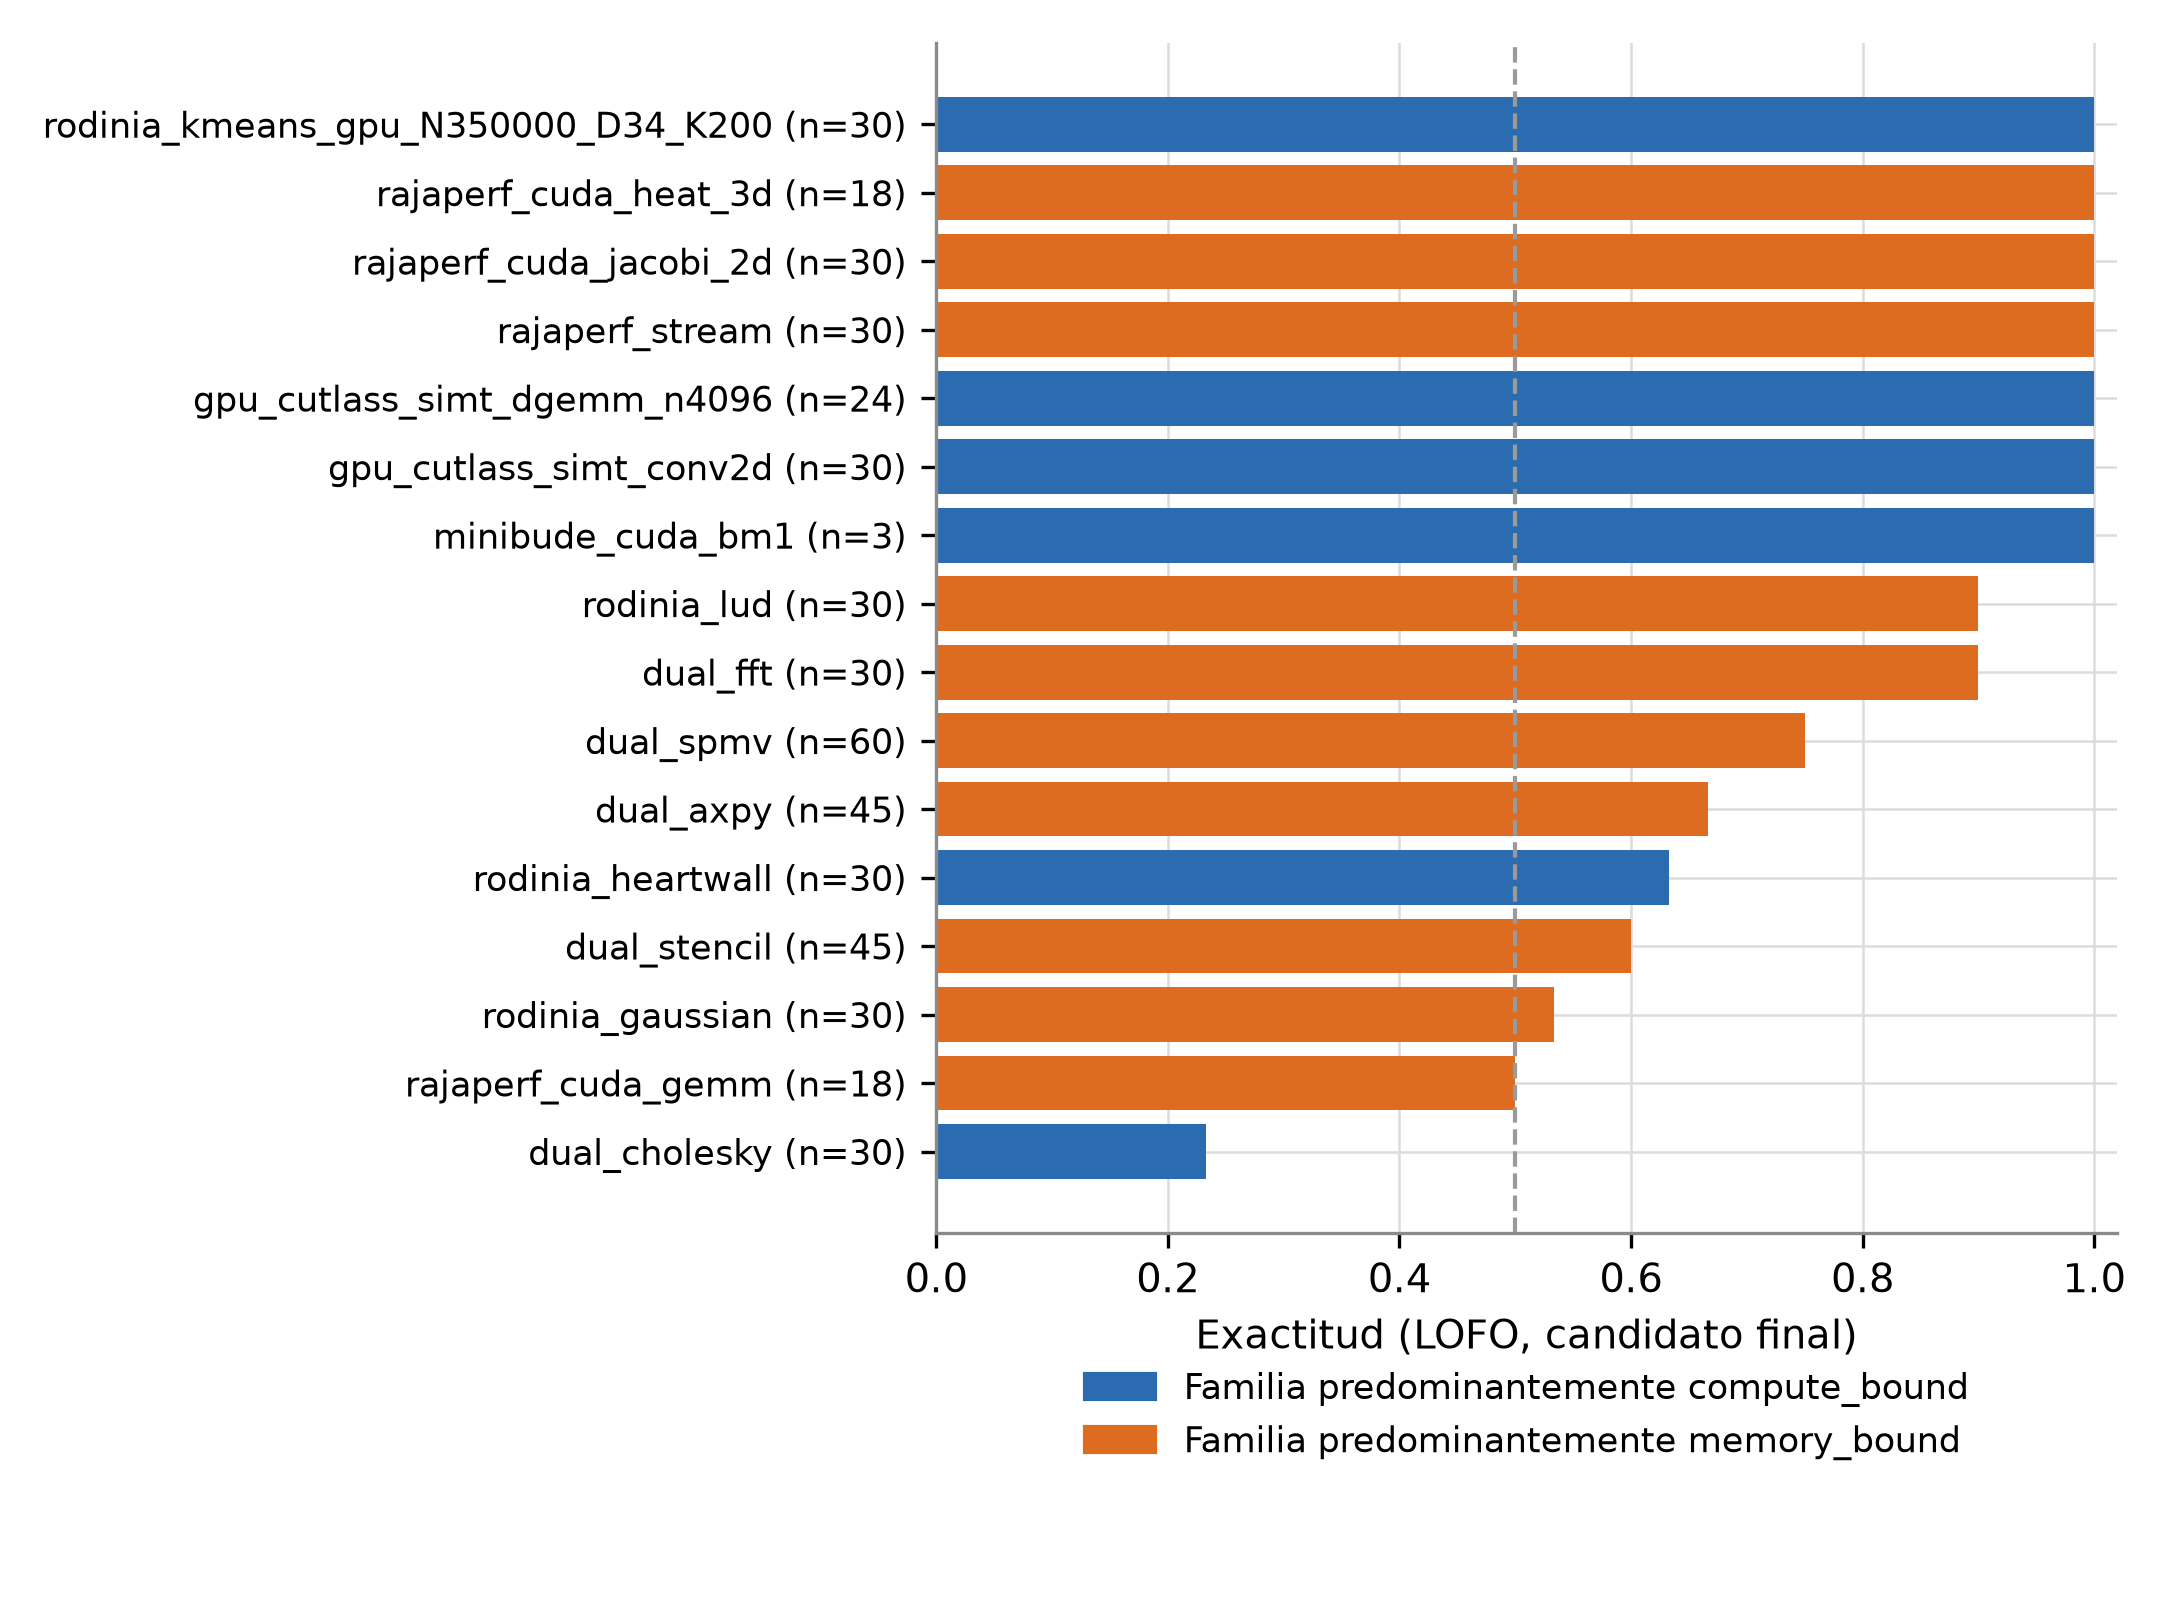
\includegraphics[width=\textwidth]{figuras/fig_gpu_resultado_por_familia_20260922.png}
    \caption[Exactitud de la referencia estática GPU por familia]{Exactitud de la regresión logística de cinco entradas por familia algorítmica, LOFO. El color indica la clase predominante real de cada familia. Fuente: elaboración propia.}
    \label{fig:gpu-resultado-por-familia}
\end{figure}





La calibración de probabilidades de la regresión logística de cinco variables, usada aquí solo como candidato estático de referencia, tiene un error de calibración esperado (ECE, calculado sobre diez rangos de confianza de igual amplitud) de 0.057. Su umbral de 0.70 sube la exactitud balanceada por celda de 0.792 a 0.846 reteniendo el 76.7\% de las corridas (Figura \ref{fig:gpu-calibracion-umbral}). La selección del modelo desplegable se reporta por separado después de aplicar el contrato de entradas invariantes.

\begin{figure}[H]
    \centering
    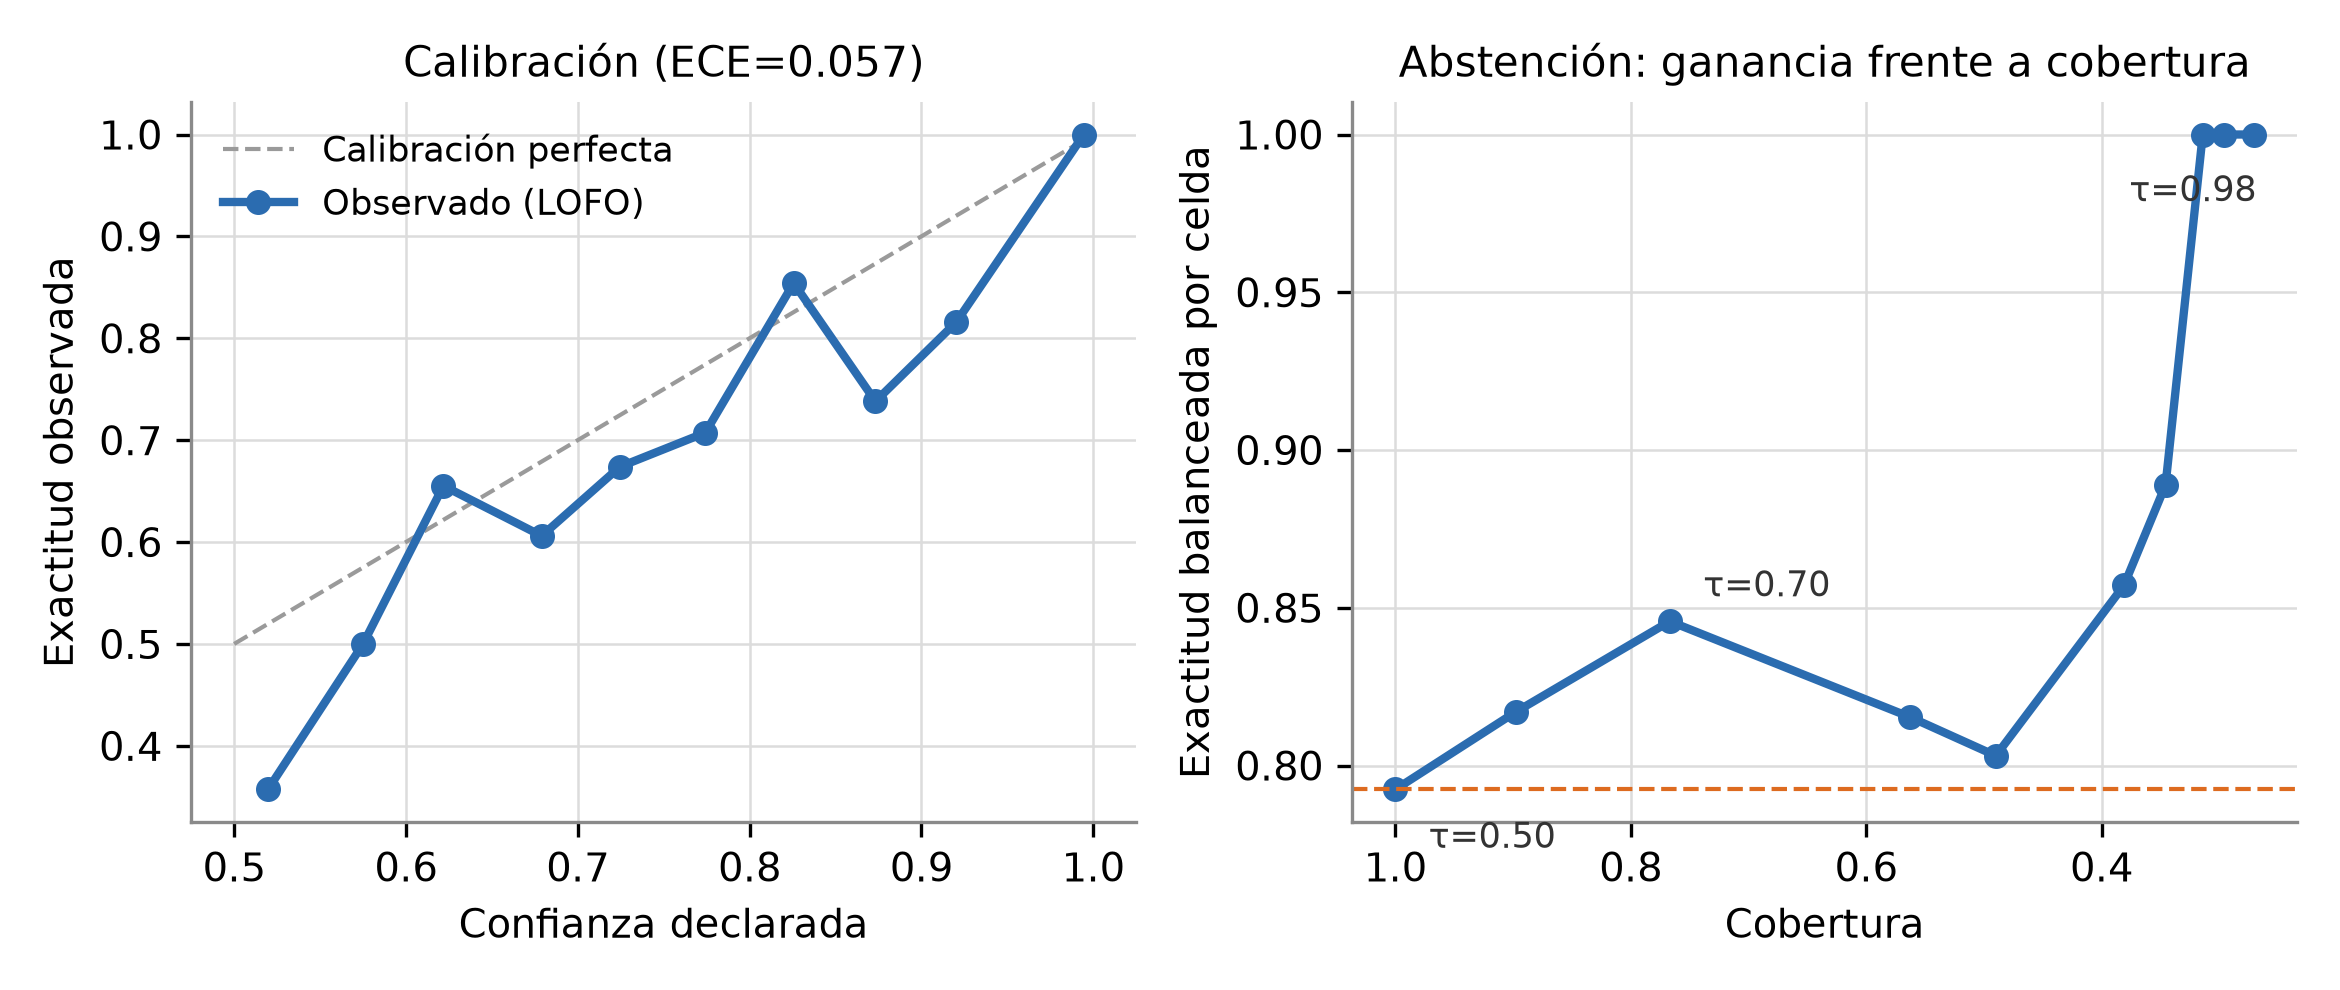
\includegraphics[width=\textwidth]{figuras/fig_gpu_calibracion_umbral_20260922.png}
    \caption[Calibración y abstención de la regresión logística GPU]{Calibración y abstención de la regresión logística de cinco entradas, candidata estática que no se despliega en el agente. Izquierda, confianza declarada contra exactitud observada, agrupada en diez rangos de igual amplitud. Derecha, exactitud balanceada por celda contra cobertura para distintos umbrales de decisión $\tau$. Fuente: elaboración propia.}
    \label{fig:gpu-calibracion-umbral}
\end{figure}

La regresión logística estática ya congelada, con sus cinco entradas, se evaluó una vez contra cuatro familias de Rodinia de una campaña de agosto (Backprop, DWT2D, LavaMD y Myocyte) que no participaron en ninguna decisión de esta ronda: ni en el umbral de aceptación de corridas, ni en la separación de familias de RAJAPerf, ni en la variable de variabilidad añadida, ni en la elección del modelo. Es el equivalente honesto a un conjunto de prueba sellado para esa referencia. Sobre 140 corridas, la exactitud global fue 0.779 (Figura \ref{fig:gpu-matriz-confusion}, panel derecho), con \textit{LavaMD} como la familia más débil (0.5) y las otras tres entre 0.81 y 0.97. Esta cifra es consistente con una validación externa independiente reportada en una versión anterior de este análisis sobre un conjunto ligeramente distinto (exactitud 0.743, misma familia más débil), lo que respalda que el resultado no es un artefacto de la partición específica de esta ronda.

\begin{figure}[H]
    \centering
    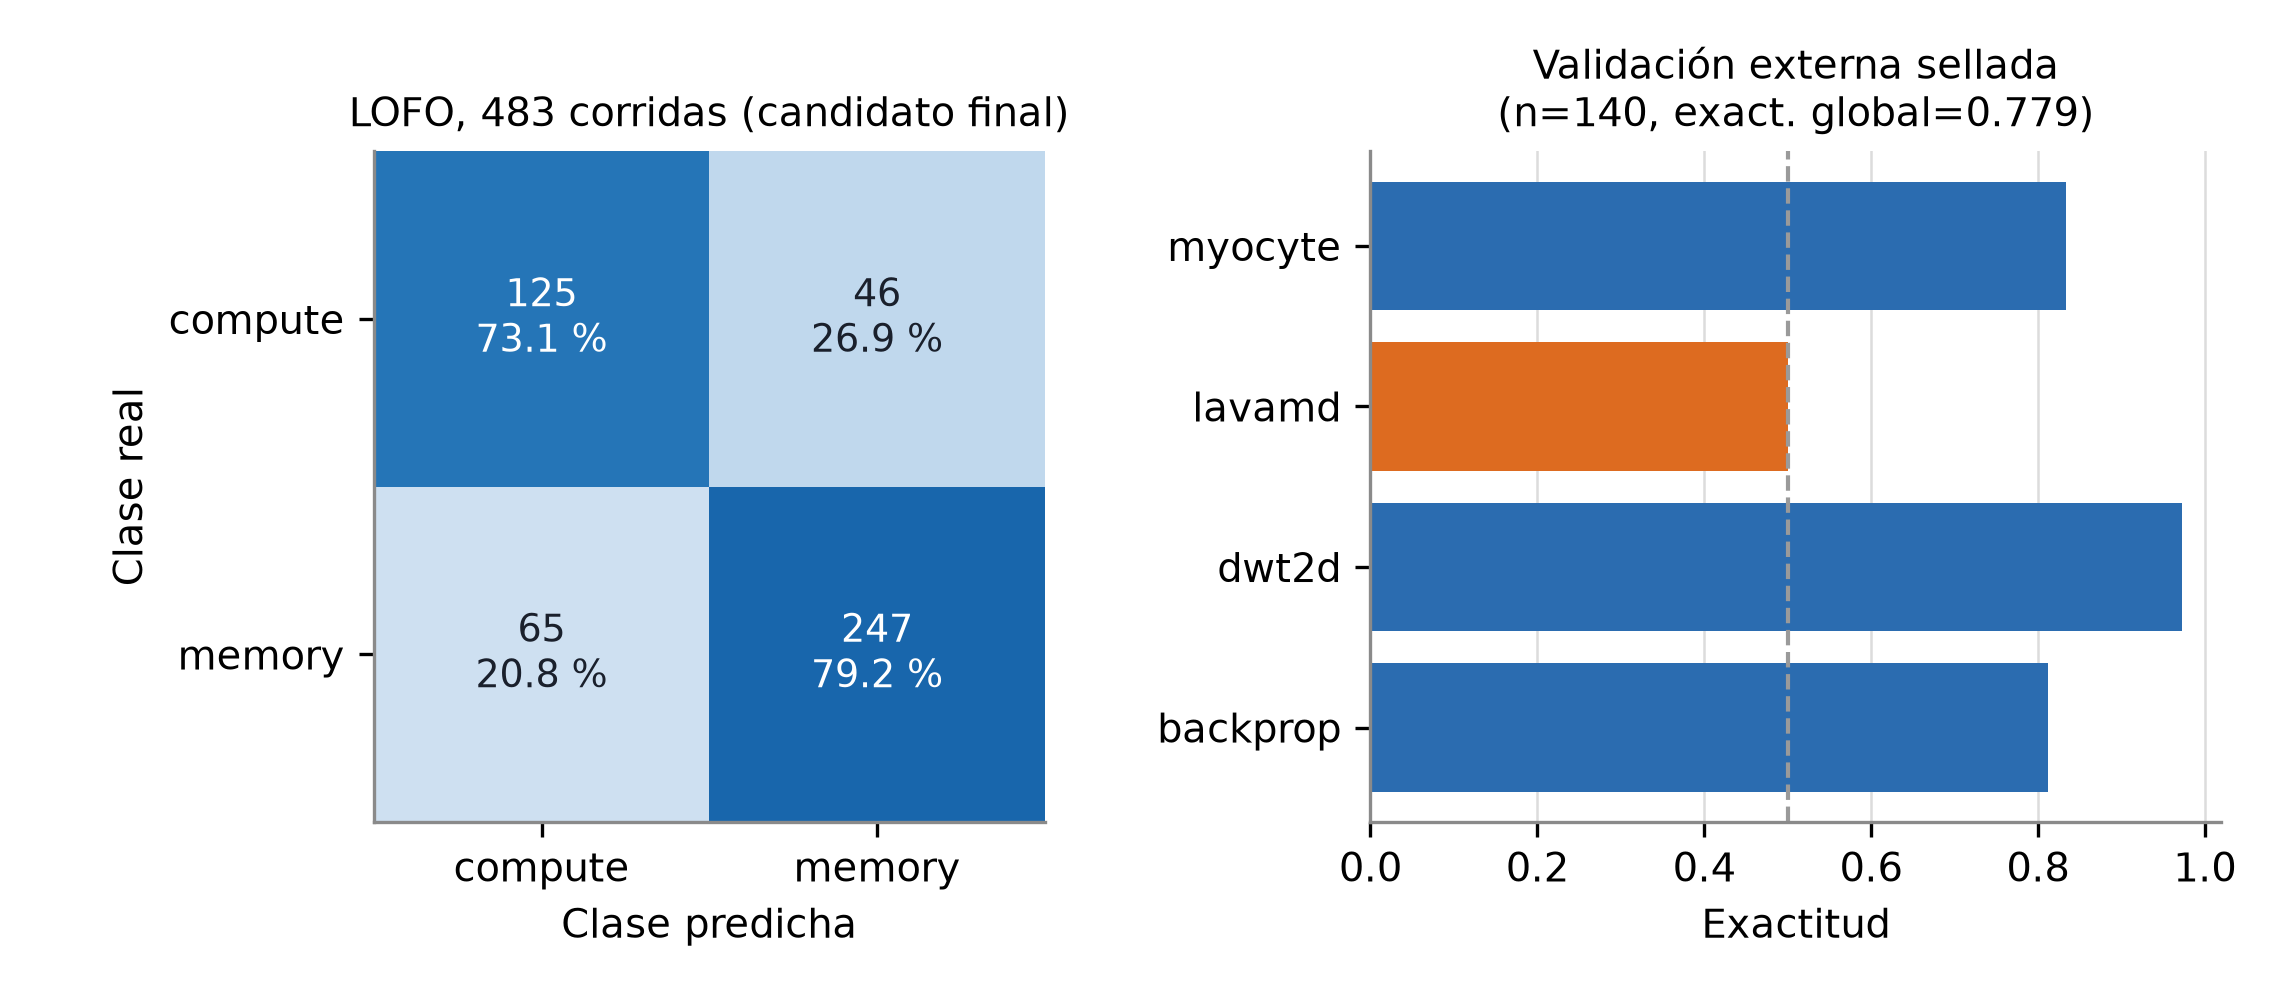
\includegraphics[width=\textwidth]{figuras/fig_gpu_matriz_confusion_20260922.png}
    \caption[Matriz de confusión y validación externa de la referencia estática GPU]{Izquierda, matriz de confusión agregada de la regresión logística de cinco entradas bajo \textit{leave-one-familia-out} (483 corridas). Derecha, exactitud por familia en la validación externa sellada (Backprop, DWT2D, LavaMD, Myocyte; 140 corridas nunca usadas en ninguna decisión de esta ronda). Fuente: elaboración propia.}
    \label{fig:gpu-matriz-confusion}
\end{figure}



\subsection{Candidato operativo de GPU: invarianza frente a la acción del agente}
\label{sec:resultados-gpu-invarianza}

La regresión logística de la subsección anterior es la referencia estática más rápida, pero el agente exige además que sus entradas no dependan del reloj que él mismo fija (sección \ref{sec:metodologia-invarianza-gpu}). La auditoría, sobre las mismas 483 corridas y sin mediciones nuevas, muestra que ese requisito cambia el modelo seleccionado (Figura \ref{fig:gpu-invarianza}). Al fijar de forma contrafactual el reloj de cada observación en 1410~MHz, la regresión logística cambia de clase el 26.7\% de sus predicciones, y su exactitud baja de 0.792 a 0.654 al excluir el reloj. El \textit{random forest} conserva el desempeño al retirar las entradas afectadas por la actuación, con 0.807 usando cinco variables, 0.812 sin reloj y 0.819 sin reloj ni potencia.

\begin{figure}[H]
    \centering
    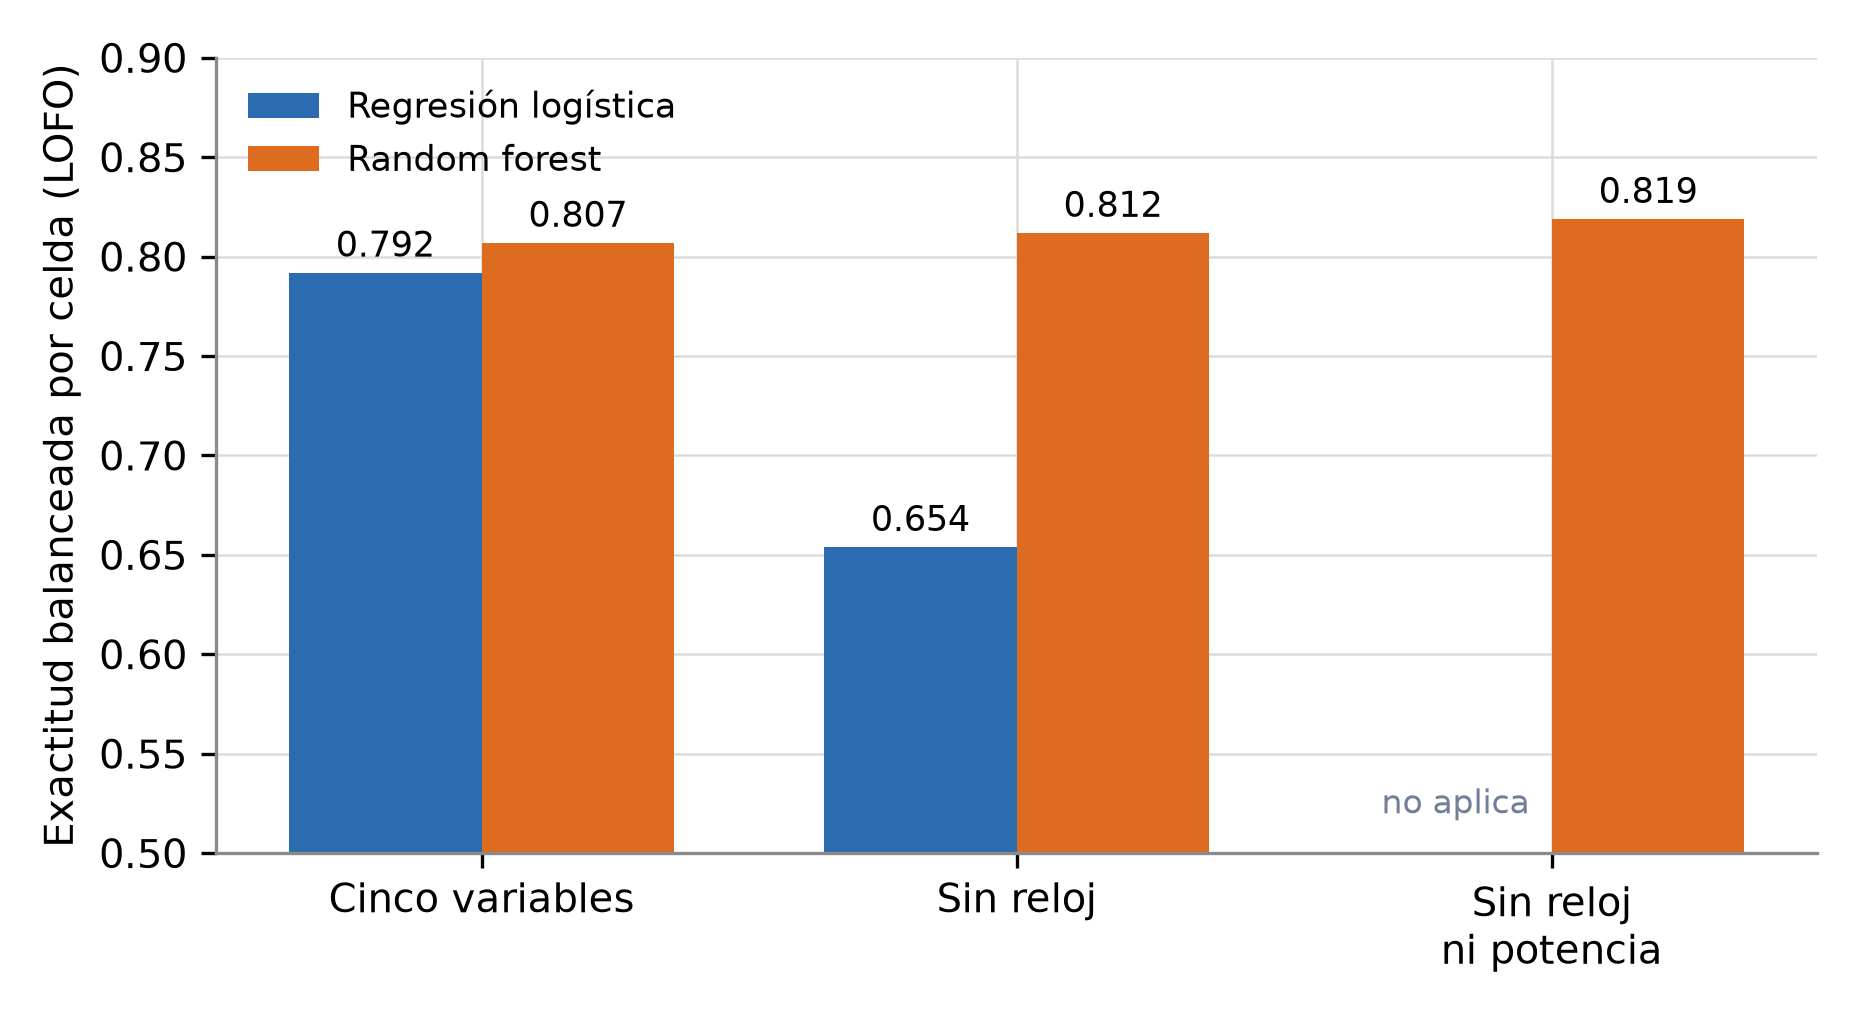
\includegraphics[width=0.85\textwidth]{figuras/fig_gpu_invarianza_reloj_20260923.png}
    \caption[Invarianza de los candidatos GPU frente al reloj]{Exactitud balanceada por celda (LOFO, 483 corridas, 16 familias) al excluir las variables que dependen de la acción del agente. Fuente: elaboración propia.}
    \label{fig:gpu-invarianza}
\end{figure}

El daemon consume el \textit{random forest} de tres entradas invariantes de la Tabla \ref{tab:gpu-modelos-operativos}. Su ECE LOFO es 0.0868 y su inferencia mediana tarda 4.7~ms, frente a los segundos requeridos para detectar y actuar sobre una fase. Con el umbral de 0.90 alcanza 0.900 de exactitud balanceada sobre el 65.7\% de las corridas aceptadas. El agente decide una sola vez por fase, por lo que una abstención no se reevalúa.

\begin{table}[H]
\centering
\caption{Modelos GPU después de aplicar el contrato de entradas del daemon. Las métricas se obtienen con LOFO sobre 483 corridas y 16 familias.}
\label{tab:gpu-modelos-operativos}
\small
\setlength{\tabcolsep}{3pt}
\begin{tabular}{@{}p{2.8cm}p{3.7cm}>{\centering\arraybackslash}p{2.1cm}>{\centering\arraybackslash}p{1.0cm}>{\centering\arraybackslash}p{1.7cm}@{}}
\toprule
\textbf{Modelo} & \textbf{Entradas} & \textbf{Exactitud balanceada} & \textbf{ECE} & \textbf{Estado} \\
\midrule
Regresión logística & Cinco señales NVML, incluidas potencia y reloj SM & 0.792 & 0.0569 & Referencia estática \\
\textit{Random forest} & Utilización GPU, utilización de memoria y desviación estándar de esta última & 0.819 & 0.0868 & Desplegado \\
\bottomrule
\end{tabular}
\end{table}

\subsection{Política de frecuencia por clase en GPU}
\label{sec:resultados-gpu-politica}

La tabla clase--frecuencia se derivó sobre las mismas 483 corridas de la sección anterior, con el kernel como unidad de comparación y el procedimiento de la sección \ref{sec:metodologia-politica-gpu}: mediana de repeticiones por kernel y nivel, prueba pareada contra \texttt{REF} e intervalo de confianza del 95\% por \textit{bootstrap}. Un cálculo preliminar emparejó en cambio, kernel por kernel, sus tres repeticiones de cada nivel contra sus tres de \texttt{REF} ($n=3$ por prueba); se descartó por responder una pregunta distinta de la que decide la tabla --- si el ruido de medición dentro de un kernel es distinguible de cero, no si el efecto generaliza entre kernels --- y se sustituye aquí por el resultado con el kernel, y su agregación por familia, como unidad.

De los 19 kernels con corridas aceptadas, uno (\texttt{minibude\_cuda\_bm1}) queda fuera por no tener más que una repetición en un solo nivel. De los 18 restantes, cuatro --- el núcleo GEMM y el \textit{stencil} de calor de RAJAPerf, y las variantes de menor tamaño de \texttt{dual\_axpy} y \texttt{dual\_stencil} --- quedan fuera de la prueba por no tener corridas en \texttt{REF} bajo la rejilla disponible, no por decisión editorial: sin \texttt{REF} no hay con qué parear. Restan 5 kernels \textit{compute\_bound} y 9 \textit{memory\_bound}, de los cuales tres pares (\texttt{dual\_axpy}, \texttt{dual\_spmv} y \texttt{dual\_stencil}, en su variante con \texttt{REF}) son el mismo algoritmo en dos tamaños de problema; la Tabla \ref{tab:gpu-politica-ic} agrega esos pares dentro de su familia (8 familias \textit{memory\_bound}, 5 \textit{compute\_bound}), con validación \textit{leave-one-familia-out} de la regla de nivel elegido.

\begin{table}[H]
\centering
\caption{Síntesis de la política GPU. Las ganancias son de EDP frente a REF; la rejilla completa se conserva en la Tabla \ref{tab:gpu-politica-detalle} del Anexo \ref{anexo:resultados-complementarios}.}
\label{tab:gpu-politica-ic}
\small
\begin{tabular}{@{}p{2.5cm}p{7.7cm}p{3.1cm}@{}}
\toprule
\textbf{Clase} & \textbf{Evidencia decisiva} & \textbf{Política} \\
\midrule
Cómputo & F1: $+2.1\%$ (IC95 $[-12.7;14.2]$, $p=0.438$); sin mejora confiable & No actuar \\
Memoria & F1: $+8.9\%$ (IC95 $[3.0;13.3]$, $p=0.020$); siete de ocho familias mejoran & Fijar F1 \\
\bottomrule
\end{tabular}
\end{table}



El resultado es \textbf{no actuar} en \textit{compute\_bound} y \textbf{actuar en F1 para \textit{memory\_bound}} (Figura \ref{fig:gpu-politica-forest}), con una ganancia agregada de 8.9\% (IC95 de 3.0 a 13.3\%, $p=0.020$, 7 de 8 familias mejoran). La validación \textit{leave-one-familia-out} --- aplicar la regla ``elegir F1'' a cada familia excluida, usando solo las siete restantes para elegirla --- confirma la dirección: siete de ocho pliegues eligen F1 de forma independiente y la ganancia realizada fuera de muestra es 6.5\% (IC95 de $-4.0$ a 13.1\%, un intervalo que roza cero por tratarse de solo ocho familias, pero consistente en signo con el resultado de la Tabla \ref{tab:gpu-politica-ic}). F2 muestra una ganancia de magnitud similar (7.4\%) pero no alcanza significancia con la familia como unidad, a diferencia del resultado preliminar por kernel: la diferencia es exactamente el efecto de dejar de contar dos veces los mismos algoritmos en dos tamaños.

\begin{figure}[H]
    \centering
    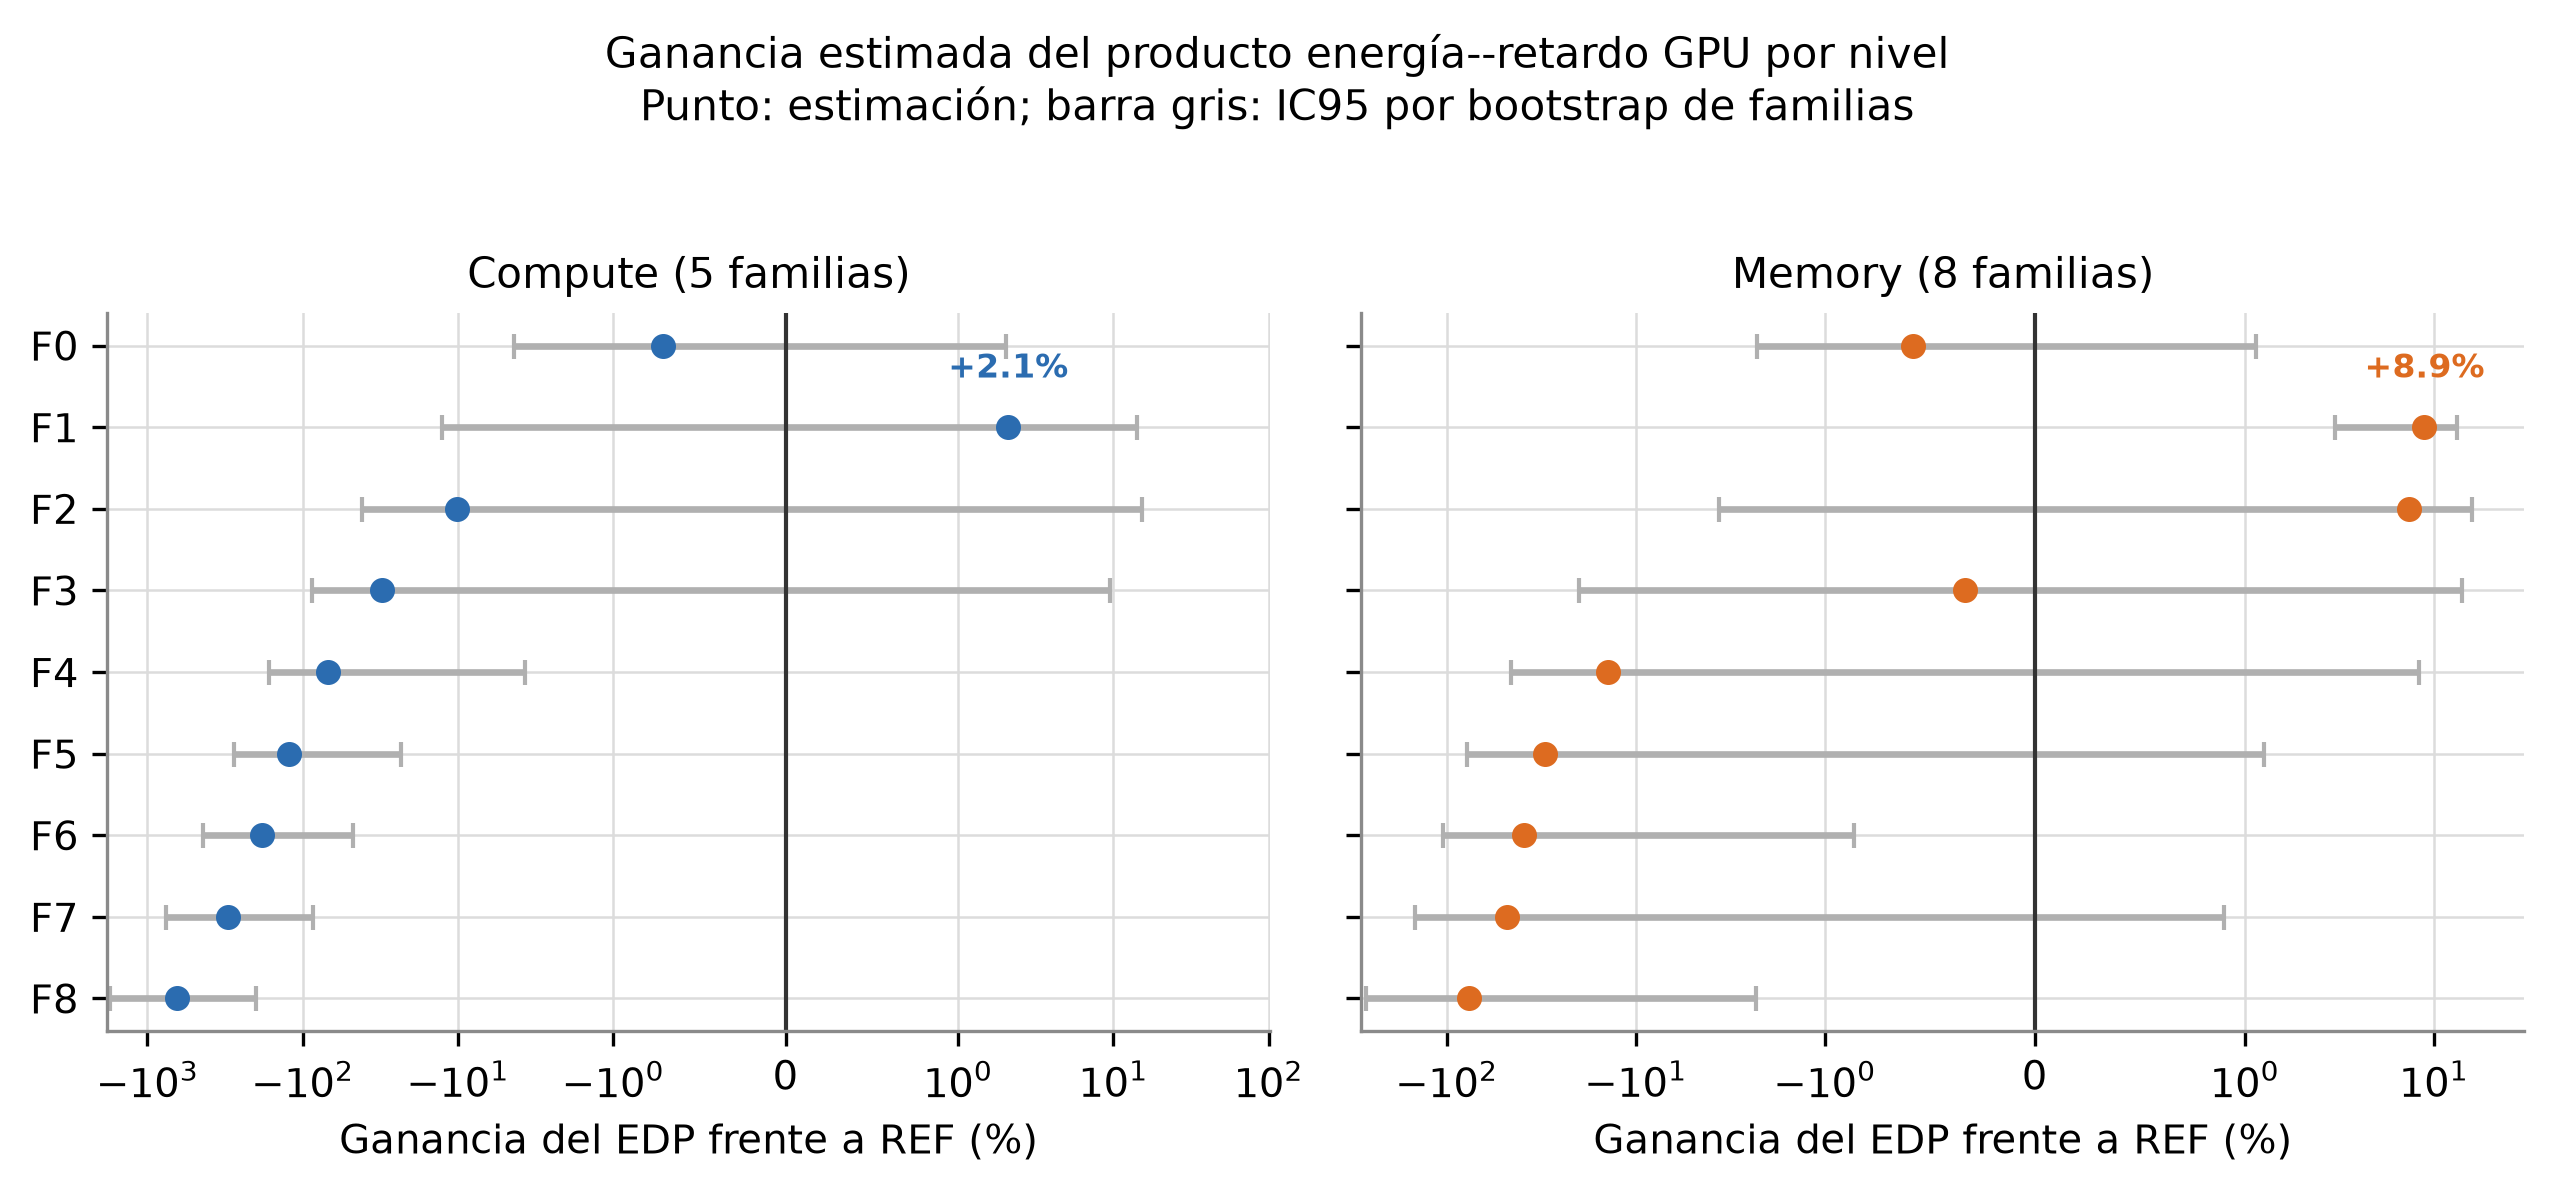
\includegraphics[width=0.94\textwidth]{figuras/fig_gpu_politica_forest_20260922.png}
    \caption[Ganancia del EDP GPU por nivel y clase, en forma de \textit{forest plot}]{La rejilla completa de la Tabla \ref{tab:gpu-politica-detalle}, en forma gráfica, con la familia como unidad. Cada punto es la ganancia estimada y la barra gris, su IC95 por \textit{bootstrap}; los rótulos señalan F1. El eje horizontal es simétrico-logarítmico para mostrar a la vez F1, cercano a cero, y F8, con pérdidas de más de un orden de magnitud en \textit{compute\_bound}. Fuente: elaboración propia.}
    \label{fig:gpu-politica-forest}
\end{figure}

En \textit{compute\_bound}, F1 parece favorable en el promedio descriptivo (+2.1\%), pero su IC95 va de $-12.7\%$ a $+14.2\%$ y la prueba pareada da $p=0.438$. No constituye una mejora confiable. Además, la validación LOFO de la regla que escoge F1 produce una ganancia realizada de $-4.8\%$ (IC95 de $-13.4$ a $0\%$): al aplicarla a una familia que no participó en elegir el nivel, empeora en promedio. Por ello el daemon conserva REF en \textit{compute\_bound}; la conclusión coincide con la de CPU.

La pendiente mediana de sensibilidad del tiempo al reloj SM es 0.837 en cómputo ($n=6$) y 0.189 en memoria ($n=12$). Por ello, en memoria puede bajarse el reloj de cómputo sin prolongar proporcionalmente la espera por el dominio de memoria, que no se varió en la campaña. La excepción es \texttt{rodinia\_gaussian}, etiquetada como memoria pero con una pendiente de 0.941 (véase el desglose en el Anexo \ref{anexo:resultados-complementarios}).

La Figura \ref{fig:gpu-politica-energia-relativa} hace visible el mismo contraste: en \textit{compute\_bound} el tiempo y el EDP crecen juntos desde F1, porque la energía apenas cae; en \textit{memory\_bound} el tiempo crece mucho más lentamente y la energía sí cae de forma sostenida hasta F3, de modo que el EDP se mantiene por debajo de 1 en F1--F2 antes de que la caída de energía se agote y el tiempo tome el control a partir de F5. Ajustando $P(f)=P_0+c\,f^{k}$ a la potencia de cada kernel frente al reloj SM --- descartando seis de los 18 kernels cuyo rango de reloj disponible (menos de siete niveles con datos) o cuyo ajuste resultante ($R^2<0.8$) no identifica los tres parámetros de forma confiable ---, el piso estático $P_0$ resulta de 38.5~W en mediana sobre los 12 kernels restantes, y representa el 55.8\% de la potencia al reloj más alto (Figura \ref{fig:gpu-politica-piso}): un margen de potencia dinámica más amplio, proporcionalmente, que el 84\% estático de CPU, consistente con que \textit{memory\_bound} sí encuentre una región de mejora que CPU no encontró en ninguna clase.

\begin{figure}[H]
    \centering
    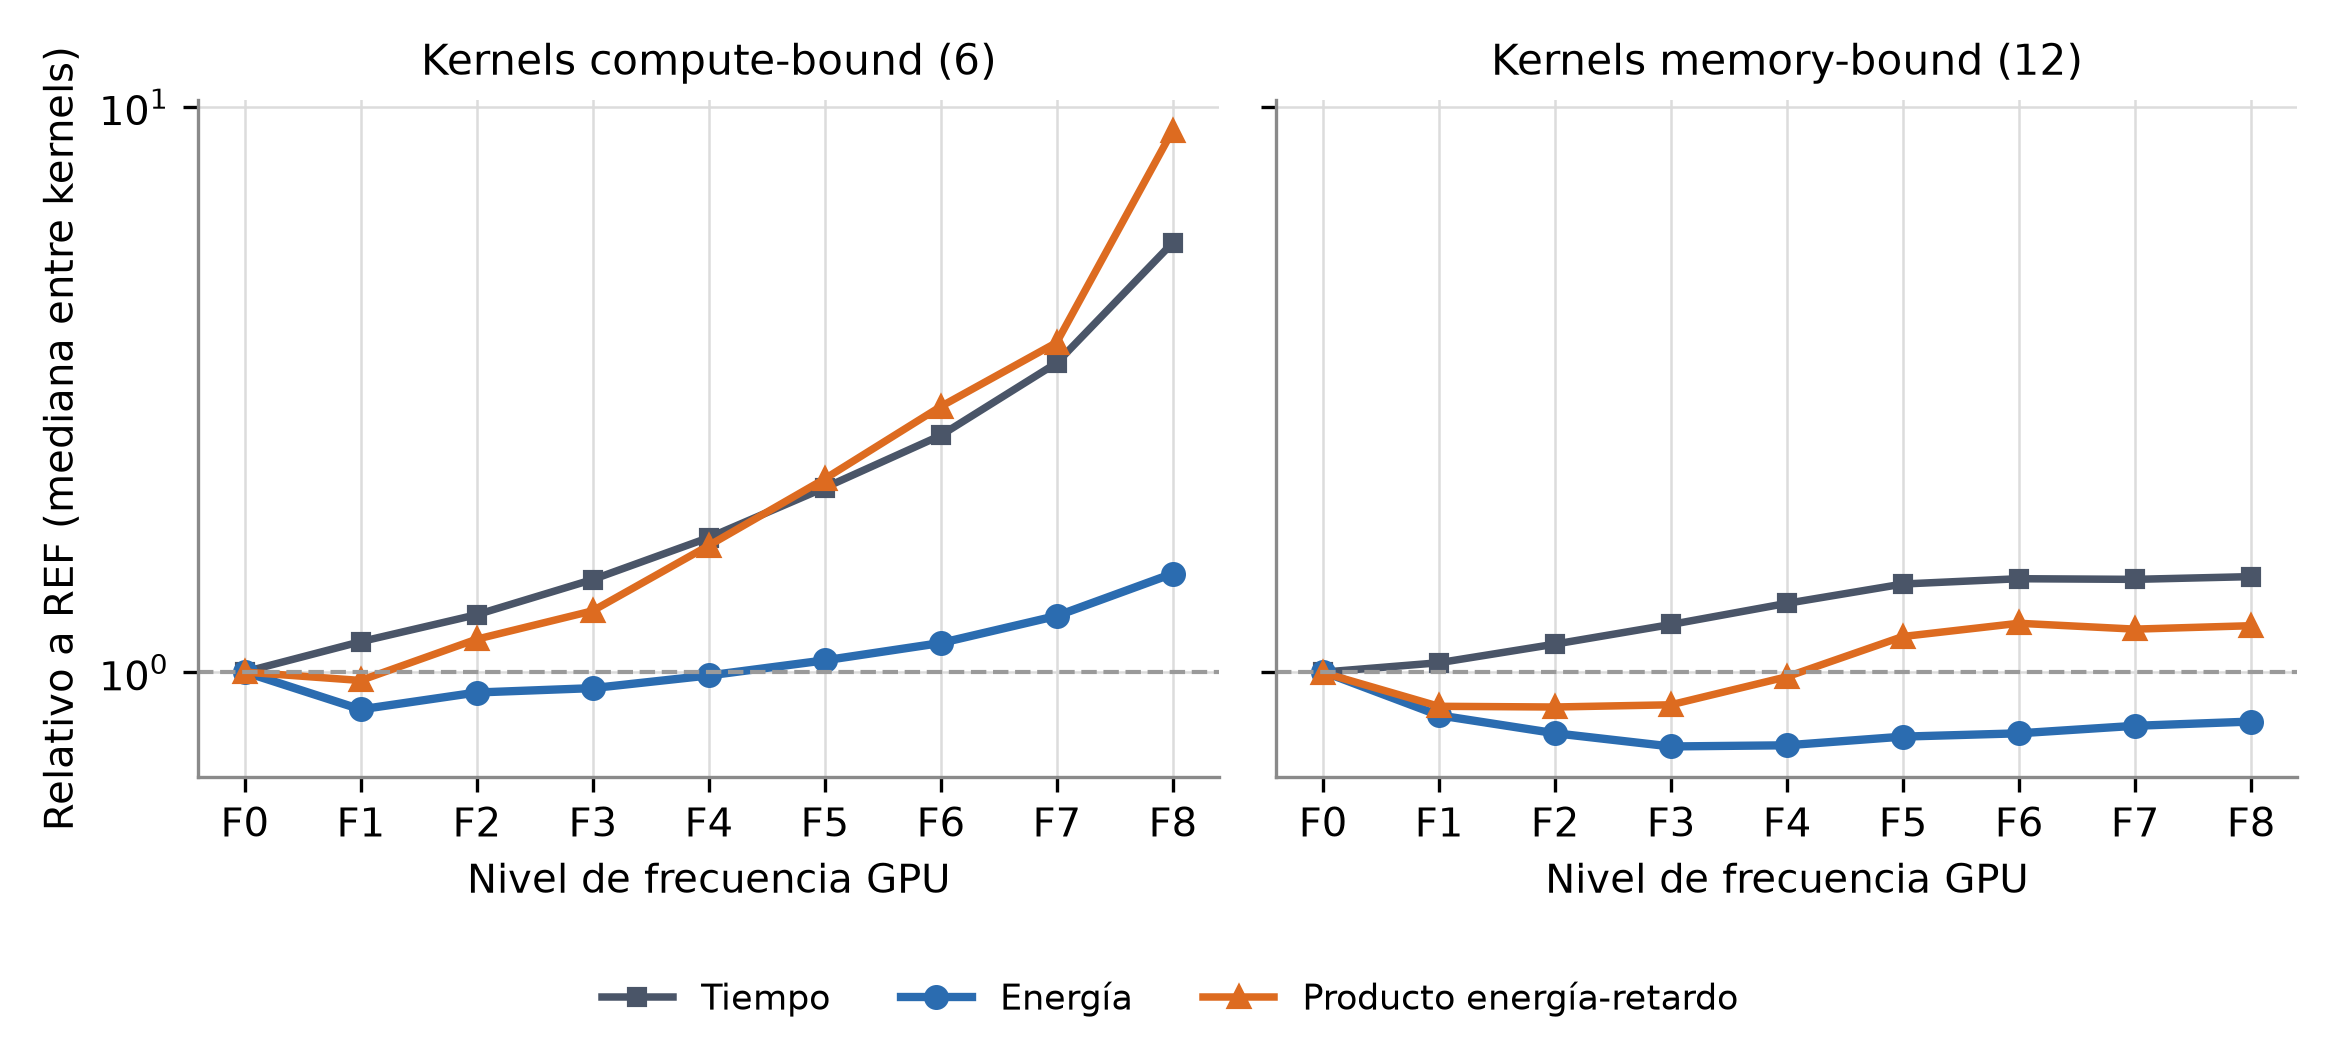
\includegraphics[width=0.94\textwidth]{figuras/fig_gpu_politica_energia_relativa_20260922.png}
    \caption[Tiempo, energía y EDP relativos por nivel de frecuencia GPU]{Mediana entre kernels del tiempo, la energía y el producto energía--retardo de cada nivel, relativos a \texttt{REF}, para las dos clases (5 y 9 kernels con corridas en \texttt{REF}, kernel como unidad, descriptivo; la significancia se evalúa por familia en la Tabla \ref{tab:gpu-politica-ic}). El eje vertical es logarítmico. Fuente: elaboración propia.}
    \label{fig:gpu-politica-energia-relativa}
\end{figure}

\begin{figure}[H]
    \centering
    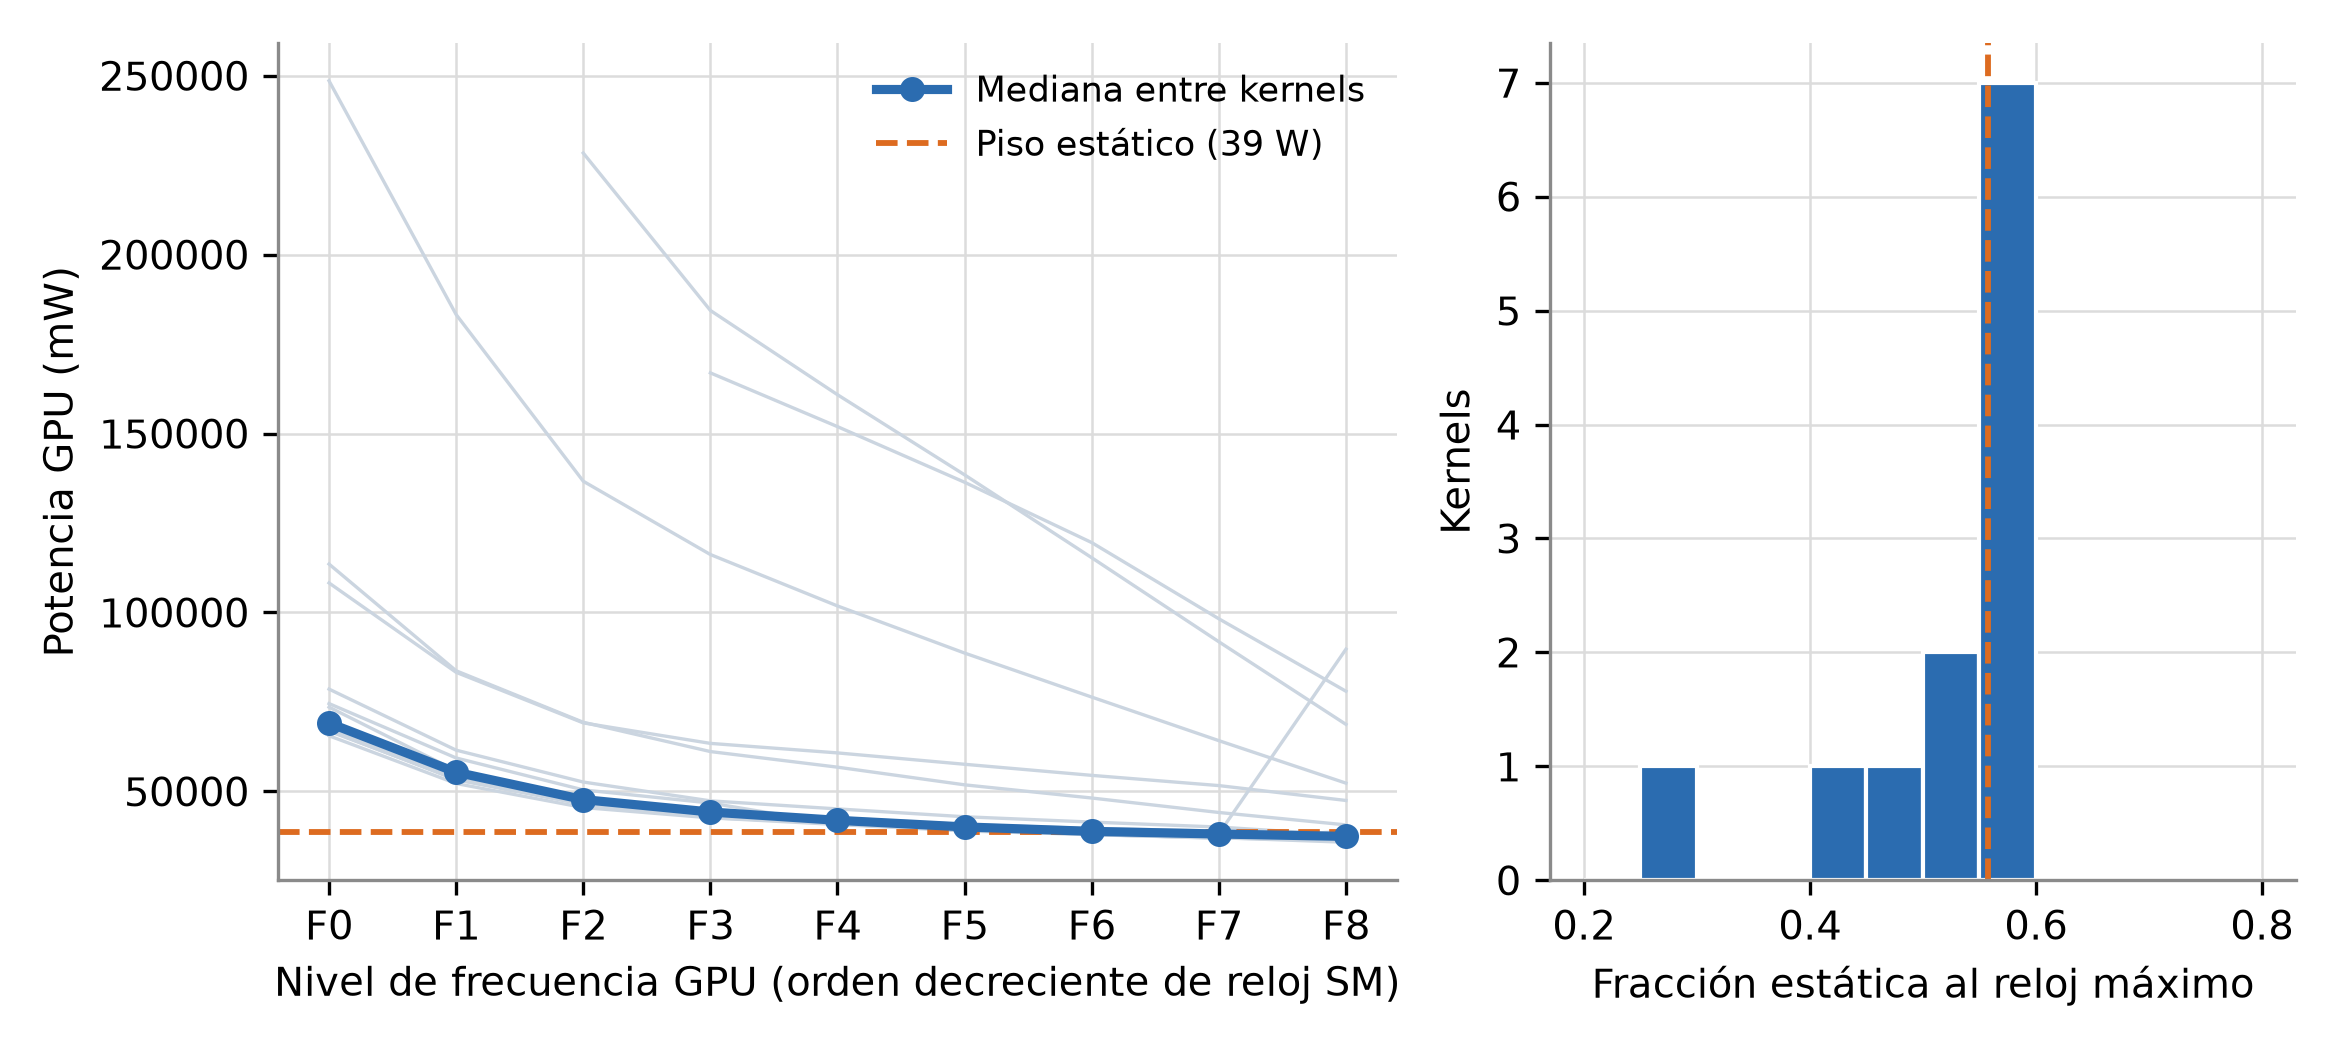
\includegraphics[width=0.94\textwidth]{figuras/fig_gpu_politica_piso_20260922.png}
    \caption[Potencia de GPU frente al reloj SM y piso estático]{Izquierda: potencia media de GPU de cada kernel (líneas grises) y su mediana en cada nivel, con el piso estático ajustado (12 kernels con ajuste identificable). Derecha: distribución entre esos kernels de la fracción de la potencia al reloj más alto que corresponde al piso. Fuente: elaboración propia.}
    \label{fig:gpu-politica-piso}
\end{figure}

En la validación por familia retirada, siete de ocho familias de memoria realizaron ganancias de 4.2 a 14.8\%; \texttt{rodinia\_gaussian} perdió 27.3\%. Su tiempo responde al reloj como una carga de cómputo pese a su etiqueta de memoria. Se conservó en el análisis: excluirla después de observar la pérdida sesgaría la política.

\subsection{Continuidad de la ruta CUPTI}
\label{sec:resultados-gpu-hiperparam}

La limitación observada en el reanálisis no invalida el uso de NVML como proxy ligero, pero delimita lo que puede esperarse de él. NVML mide efectos agregados de toda la GPU y no expone FLOPs, bytes movidos, ocupación ni la identidad del kernel activo en cada instante. Un sondeo más frecuente produce más lecturas del mismo estado agregado, no reconstruye los límites de los lanzamientos. Por ello se implementó una vía independiente, basada en la API de actividades de CUPTI, para ubicar en el tiempo real cada lanzamiento CUDA de una corrida y combinarlo con un modelo analítico de trabajo por lanzamiento \cite{CUPTI2026}. La biblioteca de captura se inyecta en el proceso CUDA medido, no en el proceso recolector, porque el lanzador separa ambos con \texttt{fork}+\texttt{exec}. Una auditoría de cobertura, de tipo \textit{fail-closed}, exige que todo kernel GPU del catálogo tenga registrado un modelo analítico de FLOPs y bytes por lanzamiento antes de permitir que una campaña con esta traza comience; diecinueve kernels del catálogo lo tienen.

Con esa infraestructura se ejecutó una campaña sobre el catálogo GPU completo, 544 corridas planificadas. La captura de la traza fue correcta: la corrida de \textit{rodinia\_gaussian} registró 8197 eventos CUPTI, consistentes con los aproximadamente 8190 lanzamientos esperados de \texttt{Fan1}/\texttt{Fan2} para una eliminación gaussiana de tamaño 4096. El mecanismo de captura por lanzamiento funciona como fue diseñado.

La campaña CUPTI capturó los lanzamientos, pero su eje de frecuencia no fue válido: con solicitudes de 700 y 1200~MHz, el reloj observado permaneció en 765~MHz. Ninguna ventana cumplió la tolerancia de reloj para entrenar por nivel. Se conservaron las trazas y calibraciones; una verificación posterior volvió a encontrar operativo el candado (sección \ref{sec:resultados-agente-candado}). Por tanto, el fallo afecta esa campaña, no la política GPU derivada de las 483 corridas previas.

CUPTI mantiene dos funciones futuras diferenciadas, independientes del resultado anterior. Su perfilado de contadores puede construir una intensidad operacional y una etiqueta Roofline por kernel en una campaña controlada. Su API de actividades, ya implementada, puede registrar los límites temporales de lanzamientos y transferencias necesarios para asociar esa etiqueta con el segmento NVML de la misma fase. La granularidad fina requiere ambas fuentes en la misma campaña: sin el perfilado no se conoce la clase física de cada fase, y sin la traza no se sabe qué parte de la telemetría corresponde a esa fase. Ninguna de estas funciones convierte automáticamente a CUPTI en una entrada del clasificador en producción, que debe conservar únicamente señales ligeras de NVML. La reconstrucción del eje de frecuencia de esa campaña y una nueva evaluación de etiquetas por fase con CUPTI quedan como extensiones; la política de frecuencia GPU de este trabajo se obtuvo de la campaña anterior válida.

\section{Resultados del agente de control}
\label{sec:resultados-agente}

Esta sección reporta la verificación del agente de la Fase 3 en \texttt{paccaA100}, antes de la evaluación de la Fase 4. Todas las pruebas usaron el nodo en asignación exclusiva y restauraron el estado de frecuencia al terminar.

\subsection{Candado de reloj de GPU y premisa física de la política}
\label{sec:resultados-agente-candado}

Con una carga sintética de fases controladas se comprobó que, al fijar el reloj con \texttt{nvidia-smi -lgc}, el reloj observado coincide con el solicitado en los seis valores probados (1410, 1260, 1110, 810, 510 y 210~MHz), y que el rendimiento responde con la forma que supone la política (Figura \ref{fig:agente-candado}): el de una carga \textit{compute\_bound} escala aproximadamente con el reloj, mientras que el de una carga \textit{memory\_bound} no cae hasta llegar a 510~MHz. Es la premisa física de bajar el reloj en la clase \textit{memory\_bound} sin costo de tiempo, medida sobre el mismo instrumento que aplicará el agente.

\begin{figure}[H]
    \centering
    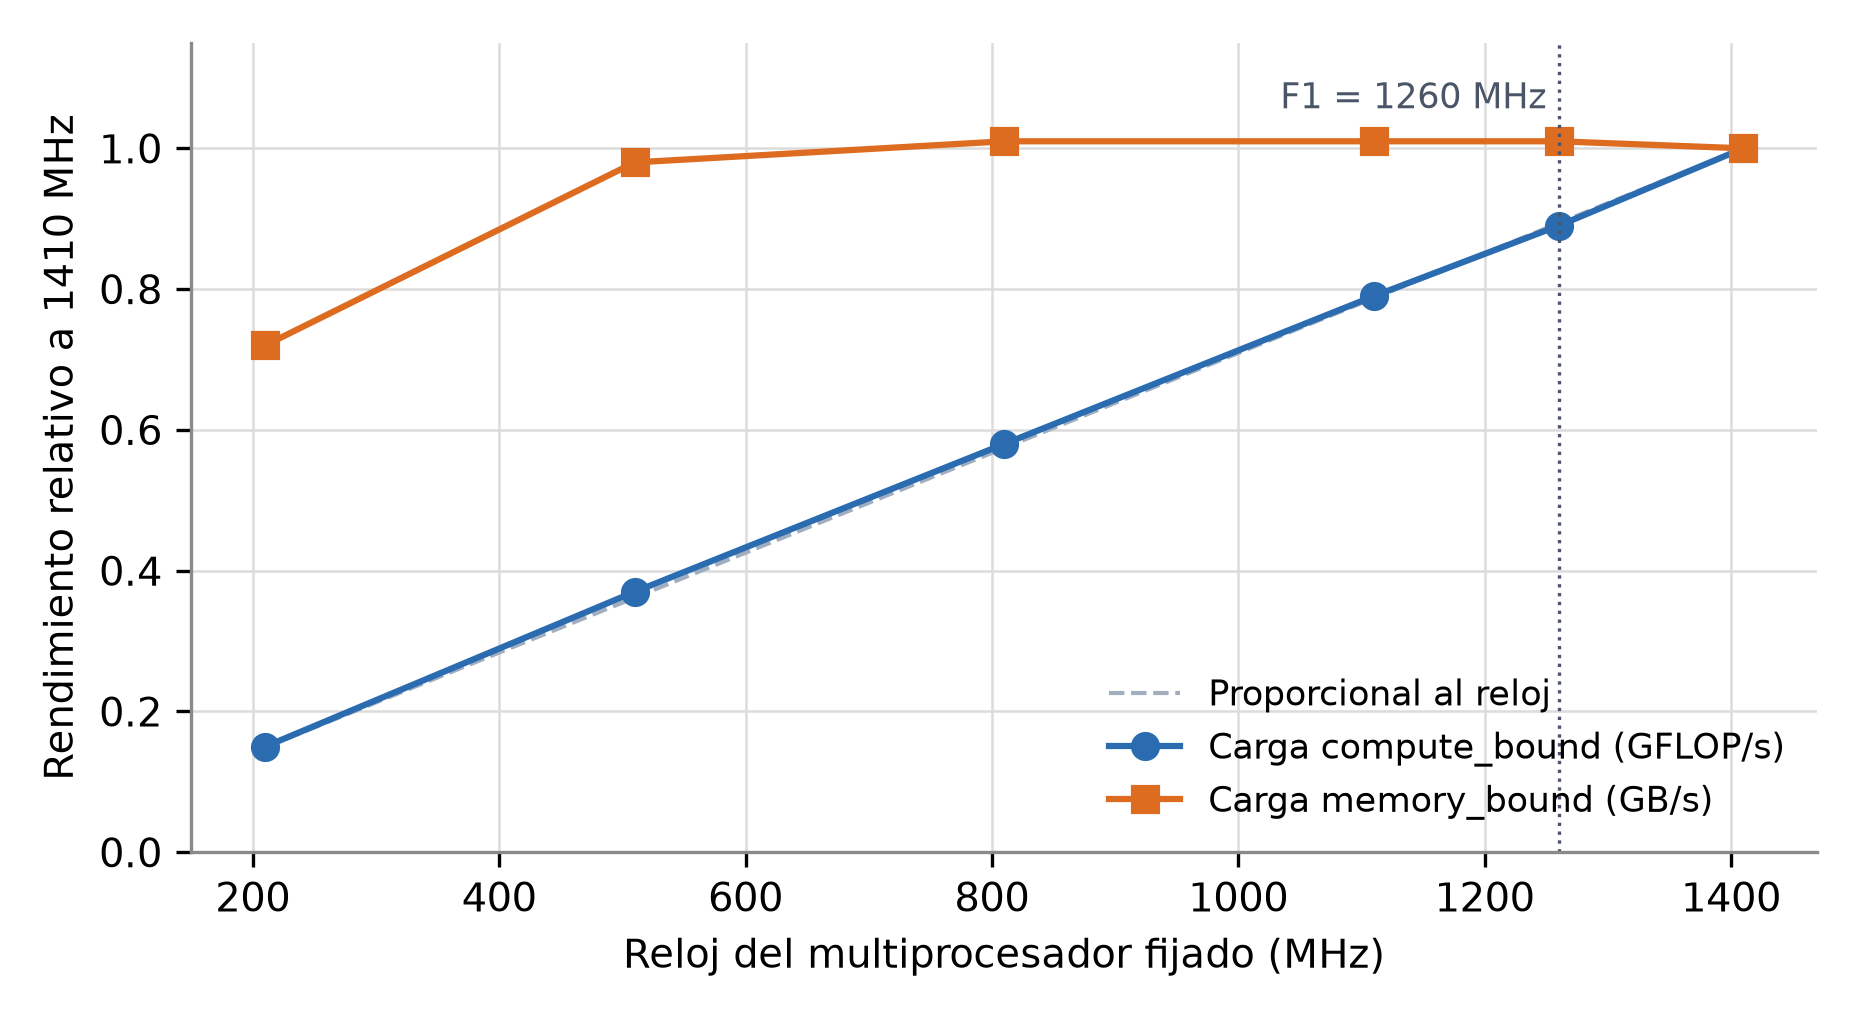
\includegraphics[width=0.85\textwidth]{figuras/fig_gpu_candado_rendimiento_20260923.png}
    \caption[Rendimiento de GPU con el reloj fijado]{Rendimiento relativo al reloj de 1410~MHz con el reloj de GPU fijado, para una carga \textit{compute\_bound} y una \textit{memory\_bound}; la línea discontinua es la proporcionalidad exacta al reloj. Fuente: elaboración propia.}
    \label{fig:agente-candado}
\end{figure}

\subsection{Latencias de conmutación y sobrecarga}
\label{sec:resultados-agente-latencias}

La Tabla \ref{tab:agente-latencias} resume las latencias de conmutación y la sobrecarga de cada proceso. La permanencia mínima entre cambios de reloj en GPU se fijó en 10 veces la latencia de conmutación observada, es decir, 3.7~s. La sobrecarga en energía de paquete del brazo \textit{sombra} frente al \textit{base} se mide en la Fase 4.

\begin{table}[H]
\centering
\caption{Latencias de conmutación y sobrecarga del agente en \texttt{paccaA100}.}
\label{tab:agente-latencias}
\small
\setlength{\tabcolsep}{3pt}
\begin{tabular}{@{}>{\raggedright\arraybackslash}p{1.6cm}>{\raggedright\arraybackslash}p{8.5cm}>{\centering\arraybackslash}p{3.0cm}@{}}
\toprule
\textbf{Dispositivo} & \textbf{Magnitud} & \textbf{Valor} \\
\midrule
GPU & Comando de fijado de reloj & $\approx$ 50~ms \\
GPU & Reloj observado en el valor pedido (tras el comando) & 70 a 80~ms \\
GPU & Uso de CPU del proceso con la GPU en reposo & 0.0 a 0.1\% de un núcleo \\
CPU & Escritura secuencial de límites en los núcleos delegados & 27.9~ms \\
CPU & Escritura en paralelo, un hilo por núcleo & 2.85~ms \\
CPU & Inferencia del clasificador (percentil 50 / 99) & 16.4 / 19.3~$\mu$s \\
\bottomrule
\end{tabular}
\end{table}

\subsection{Restauración bajo terminación anómala y coordinación}
\label{sec:resultados-agente-restauracion}

La Tabla \ref{tab:agente-restauracion} resume las pruebas de restauración y de coordinación. En cada prueba de terminación anómala inducida (\texttt{SIGTERM} o \texttt{SIGINT}) el agente atendió la señal y devolvió el dispositivo a su estado inicial, con código de salida 0. La prueba de coexistencia ejecutó ambos procesos en brazo activo sobre la aplicación compuesta A de GPU con el piso de CPU en 3.2~GHz.

\subsection{Detección y clasificación de fase de GPU sobre aplicaciones compuestas}
\label{sec:resultados-agente-deteccion}

La Tabla \ref{tab:agente-deteccion} reporta la clasificación de fase de GPU del agente sobre las dos aplicaciones compuestas, con el umbral de abstención de 0.90. En la aplicación A, las decisiones correctas tuvieron confianza 1.00 y las abstenciones entre 0.57 y 0.67; en la aplicación B, \textit{LavaMD}, una familia inédita, se clasificó correctamente con confianza 1.00. Los conteos son pequeños y sirven para verificar el funcionamiento del detector y de la abstención; la exactitud con muestra suficiente es lo que mide la Fase 4.



\section{Evaluación del agente frente a REF (Fase 4)}
\label{sec:resultados-fase4}

Esta sección reporta la evaluación experimental del agente frente al \textit{governor} nativo con turbo (REF) en \texttt{paccaA100}, según la matriz de la sección \ref{sec:metodologia-fase4}. Se reportan la matriz inicial (escenario A), sus repeticiones de comprobación, los escenarios C, D y E, el confirmatorio de E-A, CloverLeaf y la línea base secundaria sin turbo. Las razones de las tablas se calculan sobre la mediana de cada brazo y se expresan frente a la mediana de REF de la misma combinación experimental; un valor menor que 1 es una mejora. Cuando el diseño usa bloques, también se reportan las razones emparejadas por bloque.

\subsection{Aplicaciones compuestas}
\label{sec:resultados-fase4-apps}

Cada alcance usa dos aplicaciones compuestas que encadenan kernels del catálogo, con la clase de cada fase conocida de antemano. La aplicación A reúne familias vistas durante el entrenamiento y la B familias inéditas. La Figura \ref{fig:fase4-aplicaciones} muestra la estructura de un ciclo y la Tabla \ref{tab:fase4-apps} el detalle por kernel. La fracción de tiempo en fases \textit{memory\_bound} varía entre 15\% (CPU, B) y 71\% (CPU, A), y es la magnitud que acota cuánto puede ahorrar cualquier política que solo actúe en esa clase.

\begin{figure}[H]
    \centering
    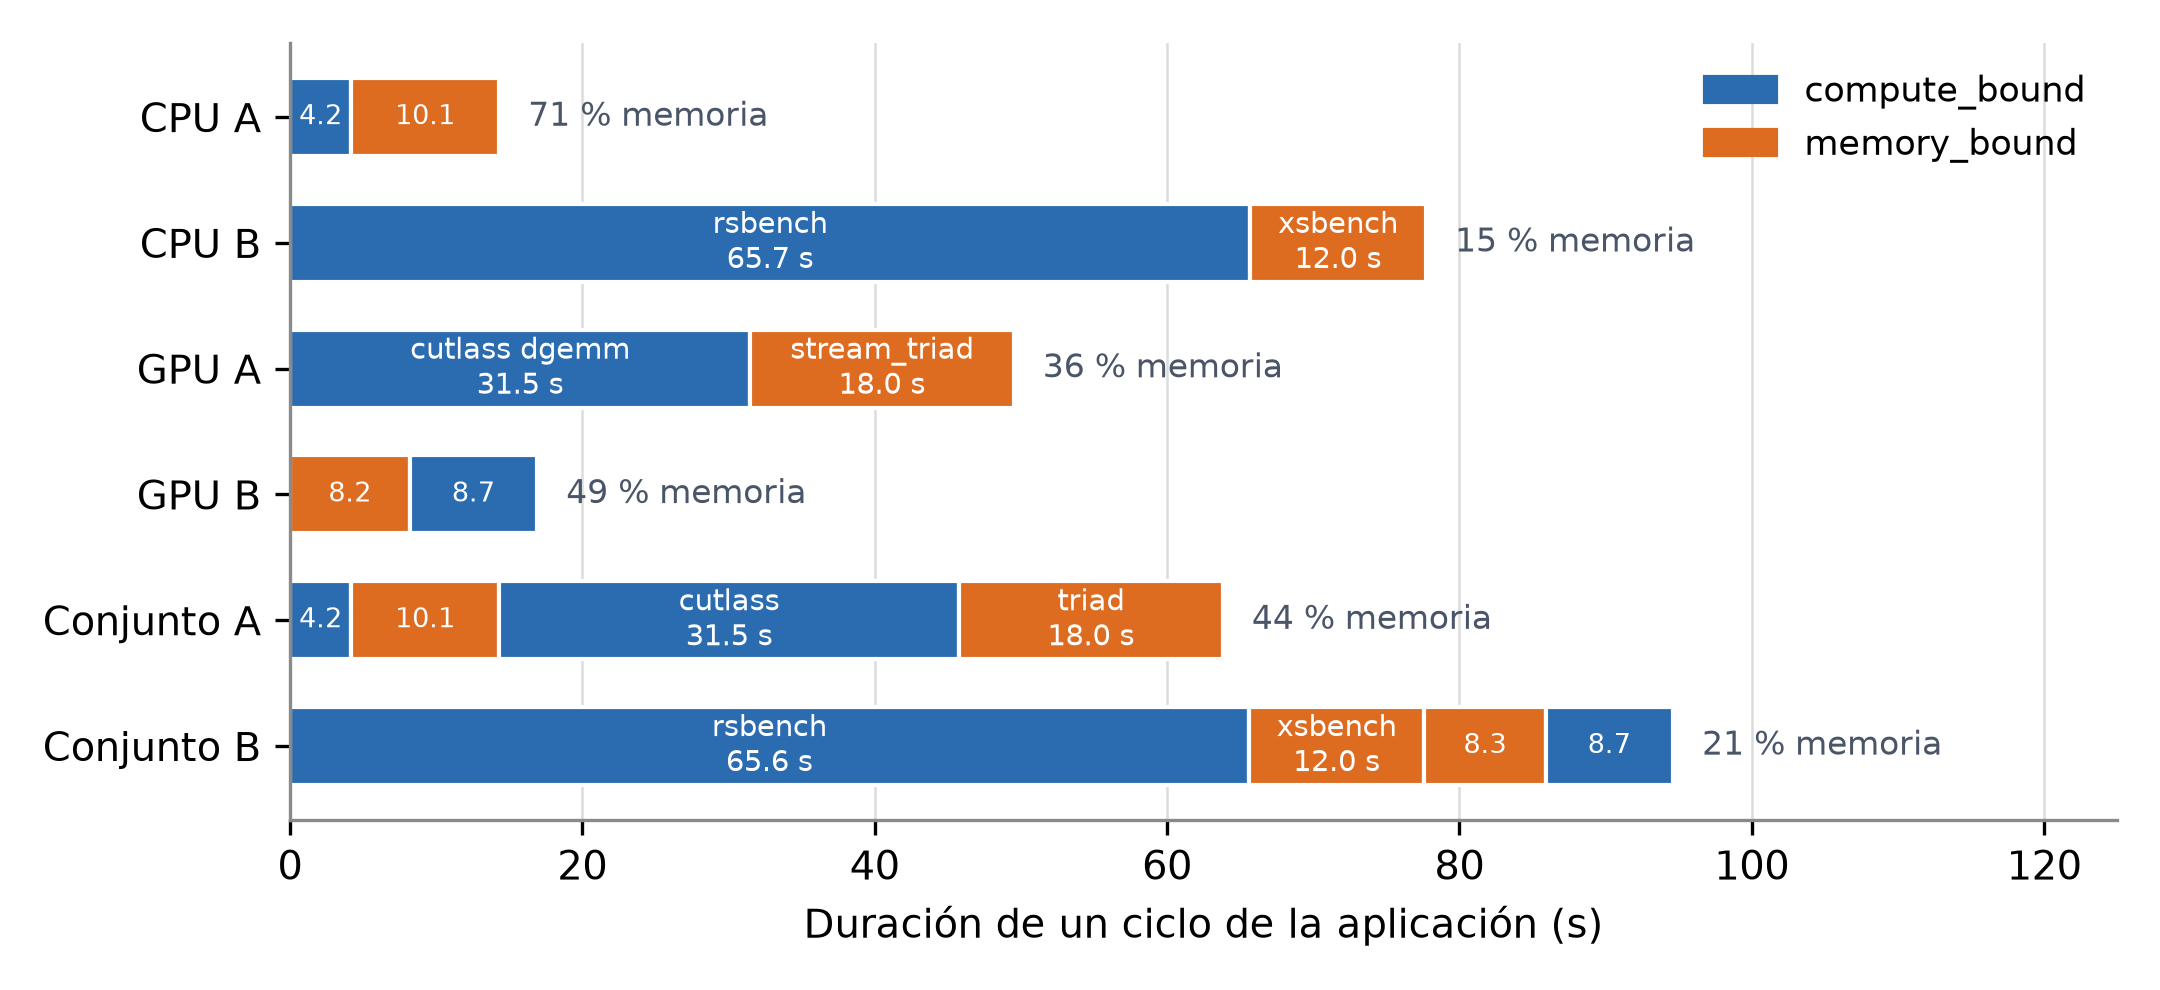
\includegraphics[width=0.94\textwidth]{figuras/fig_fase4_aplicaciones_20260924.png}
    \caption{Estructura de un ciclo de cada aplicación compuesta. Los números dentro de las barras son la duración media de cada fase en segundos; a la derecha, la fracción del ciclo en fases \textit{memory\_bound}.}
    \label{fig:fase4-aplicaciones}
\end{figure}



\subsection{Clasificación de fase con el agente en el lazo}
\label{sec:resultados-fase4-clasificacion}

La Tabla \ref{tab:fase4-clasificacion} puntúa cada decisión del agente contra la fase real en que cae su instante. En CPU las decisiones son por ventana de un milisegundo, de modo que hay decenas de miles por celda y la exactitud está ponderada por la duración de cada fase; en GPU hay una decisión por fase, con una permanencia mínima de 3.7~s.

En CPU, el agente acierta el 94\% de las decisiones sobre las familias vistas y más del 99.7\% sobre las inéditas. La diferencia favorable a las inéditas no debe leerse como mejor generalización: en la aplicación B una sola fase de cómputo ocupa el 85\% del tiempo y ponderar por ventanas la hace dominante, de modo que el resultado depende de cómo se separan esos dos kernels y no de familias arbitrarias. En GPU no hubo ninguna decisión errónea entre las que el agente tomó, pero se abstuvo con frecuencia: una de doce fases en A y entre cuatro y seis de doce en B (en el alcance conjunto, entre tres y siete de veinte). Toda fase, en cualquier alcance, recibió al menos una decisión. La exactitud del brazo activo y la del brazo sombra son indistinguibles, como corresponde a un clasificador cuya entrada no depende de la acción del agente.



\subsection{Tiempo, energía y EDP frente a REF}
\label{sec:resultados-fase4-edp}

La Tabla \ref{tab:fase4-resultados} y la Figura \ref{fig:fase4-edp} reportan la duración, las energías de CPU y de GPU por separado y las razones frente a REF de la matriz inicial. Tres hechos separan los alcances:

\begin{itemize}
    \item En \textbf{GPU} el agente activo no cambia el resultado: el EDP del nodo queda en 1.00 frente a REF en A y en B (y el brazo sombra, en 1.01 y 1.00). El agente de GPU no impone sobrecarga medible.
    \item En \textbf{CPU} el brazo activo queda entre 1.7 y 2.0 veces peor que REF en EDP, con un aumento de 15 a 25\% en tiempo y de 55 a 63\% en energía de CPU.
    \item En el alcance \textbf{conjunto} el EDP queda entre 1.3 (A) y 1.6 (B) veces el de REF. Con cinco repeticiones por brazo, la prueba de Mann--Whitney da $p = 0.0079$ en todas las comparaciones contra REF, que es el mínimo alcanzable con cinco contra cinco: las cinco corridas de cada brazo quedaron por encima de las de REF.
\end{itemize}

La descomposición por brazo indica dónde se origina la diferencia. El brazo sombra, que decide pero no escribe ninguna frecuencia, ya presenta prácticamente todo el exceso de CPU. La Tabla \ref{tab:fase4-activo-sombra} compara el brazo activo con el sombra: el efecto atribuible a la acción de frecuencia está entre $-3.3\%$ y $+2.9\%$ del EDP, es decir, de pocos puntos y de signo mixto (peor en CPU con kernels vistos, mejor con los inéditos y en el alcance conjunto). Poner F0 también en \textit{memory} (\textit{activo-F0}) o quitar el piso de coordinación (\textit{activo sin piso}) no cambia el resultado de forma apreciable.

\begin{figure}[H]
    \centering
    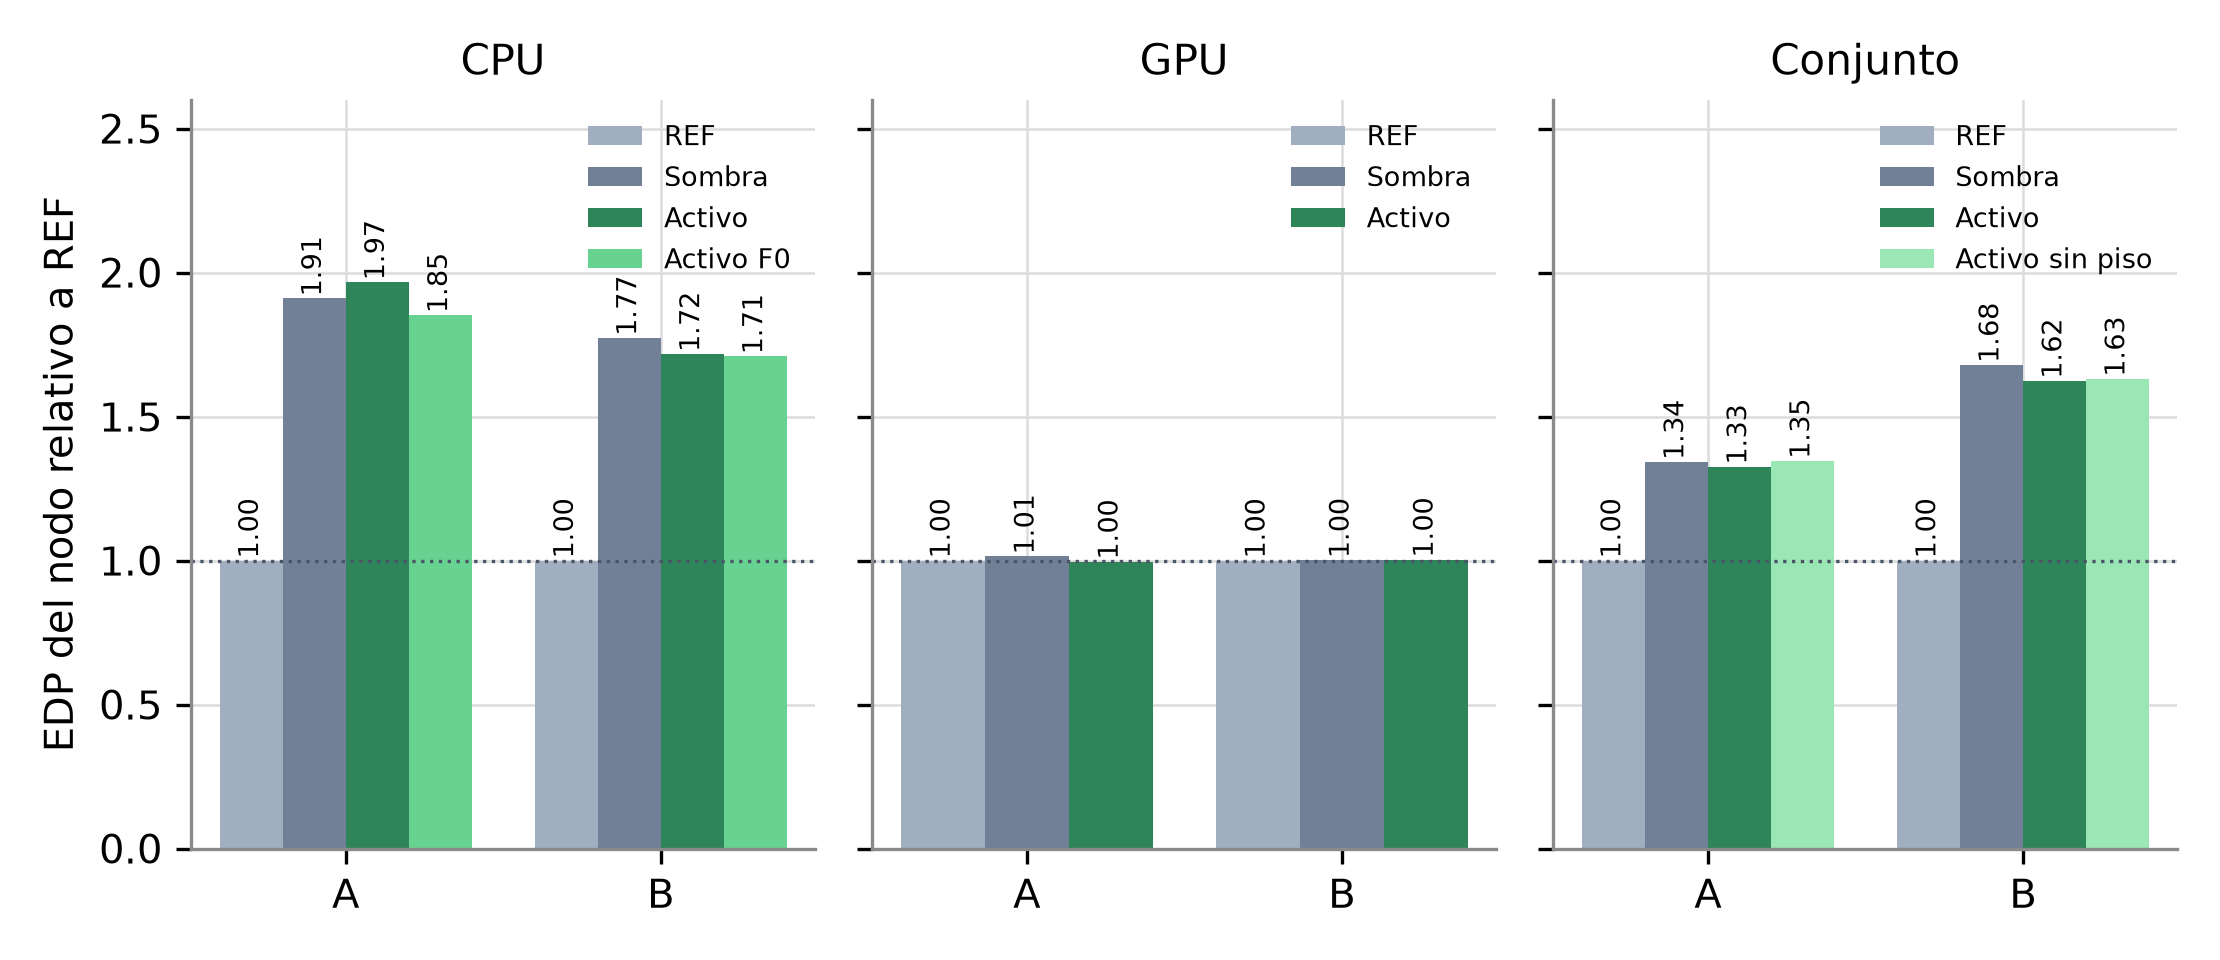
\includegraphics[width=\textwidth]{figuras/fig_fase4_edp_alcance_20260924.png}
    \caption{EDP del nodo, $(E_{\mathrm{CPU}} + E_{\mathrm{GPU}})\,T$, relativo a REF, por alcance, aplicación (A: vistos, B: inéditos) y brazo, en la matriz inicial. La línea punteada marca la paridad con REF.}
    \label{fig:fase4-edp}
\end{figure}





\subsection{Costo del agente de CPU y configuración de la inferencia}
\label{sec:resultados-fase4-costo}

La Figura \ref{fig:fase4-costo} desglosa el costo del agente. El brazo sombra permite medir el costo de mantener el agente en funcionamiento sin el efecto de la frecuencia. La causa del exceso de CPU no es el ritmo de muestreo: pasar de 1 a 10~ms reduce unas diez veces el número de decisiones y el costo no cambia (Tabla \ref{tab:fase4-costo}). Depende de la configuración del motor de inferencia. Con el conjunto de hilos por defecto, el motor de inferencia crea un hilo por núcleo que espera de forma activa entre inferencias y compite con la aplicación, que está fijada a los núcleos 0 a 3. Un único hilo de inferencia sin espera activa elimina la diferencia de tiempo (1.00 frente a REF) y reduce el sobrecosto de energía de CPU de 66\% a 6\%, y sube la exactitud de clasificación a 0.991; una explicación plausible, no verificada, es que las ventanas de contadores salen menos perturbadas cuando el agente no compite con la aplicación. Fijar el proceso consumidor a un núcleo no tiene efecto por sí solo. El agente de CPU se define, por tanto, con un hilo de inferencia; el agente de GPU no presentó este costo.



El sobrecosto de energía de CPU que queda con un hilo de inferencia no depende del periodo de muestreo: con kernels vistos, el brazo sombra queda en 1.086, 1.058 y 1.066 veces la energía de CPU de REF con periodos de 1, 10 y 100~ms (tres repeticiones cada uno), con exactitud de 97.6, 99.4 y 98.4\%. Es un costo fijo de mantener el agente, del orden de 6\%. La comparación completa del brazo activo con el agente definido con un hilo de inferencia es el escenario C (sección \ref{sec:resultados-fase4-C}).

\begin{figure}[H]
    \centering
    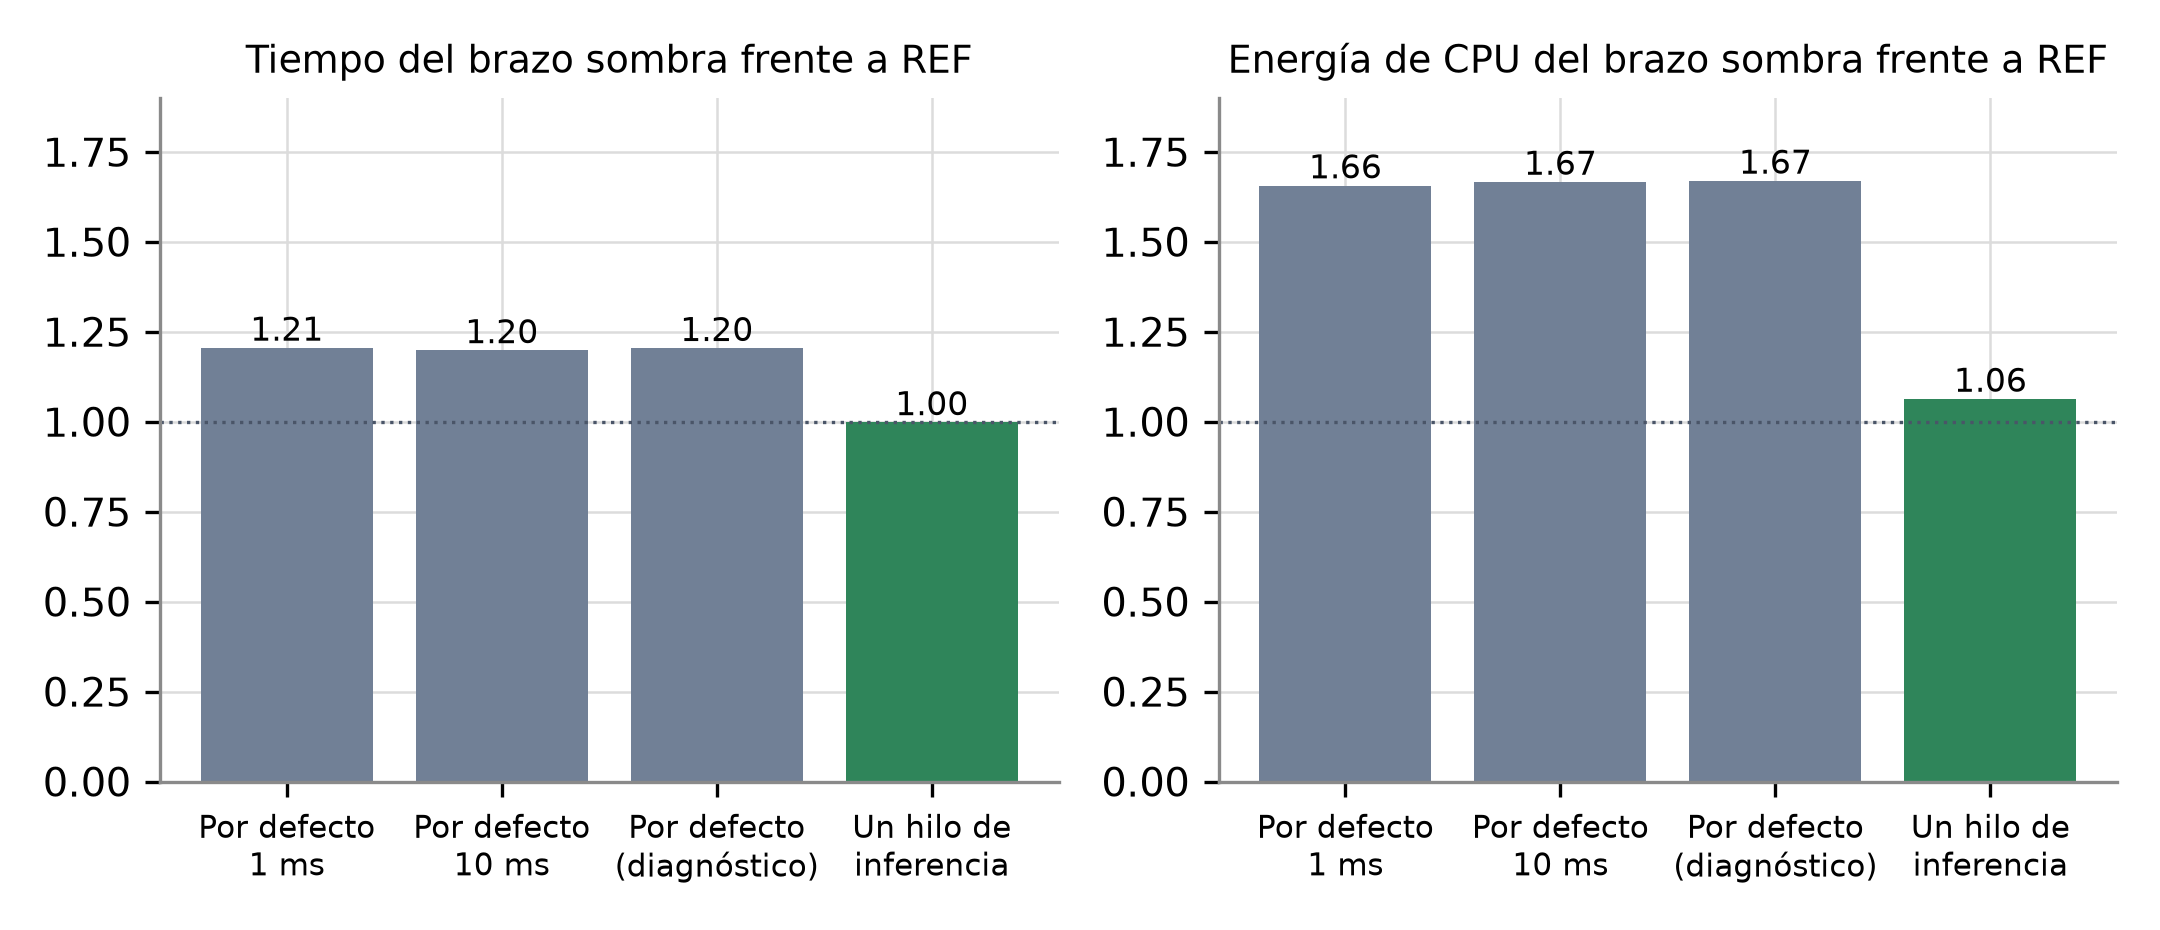
\includegraphics[width=0.94\textwidth]{figuras/fig_fase4_costo_agente_cpu_20260924.png}
    \caption{Costo del brazo sombra frente a REF en CPU con kernels vistos (A), por configuración de la inferencia y periodo de muestreo.}
    \label{fig:fase4-costo}
\end{figure}

\subsection{Potencial de la GPU}
\label{sec:resultados-fase4-gpu}

La ganancia máxima que la política de GPU puede aportar está acotada por la Fase 2: fijar el reloj en F1 (1260~MHz) durante fases \textit{memory\_bound} mejora el EDP en 8.9\% (IC95 3.0 a 13.3\%), y los niveles más bajos no mejoran o empeoran (Figura \ref{fig:fase4-gpu}, izquierda). El efecto sobre una aplicación completa se reduce por la fracción de su tiempo en memoria. Con 36\% (A) y 49\% (B) de fases \textit{memory\_bound}, la ganancia esperada del nodo es de 3.2\% y 4.3\%. La ganancia medida fue de 0.4\% en A y de $-0.3\%$ en B (Figura \ref{fig:fase4-gpu}, derecha), indistinguibles de cero con tres repeticiones.

\begin{figure}[H]
    \centering
    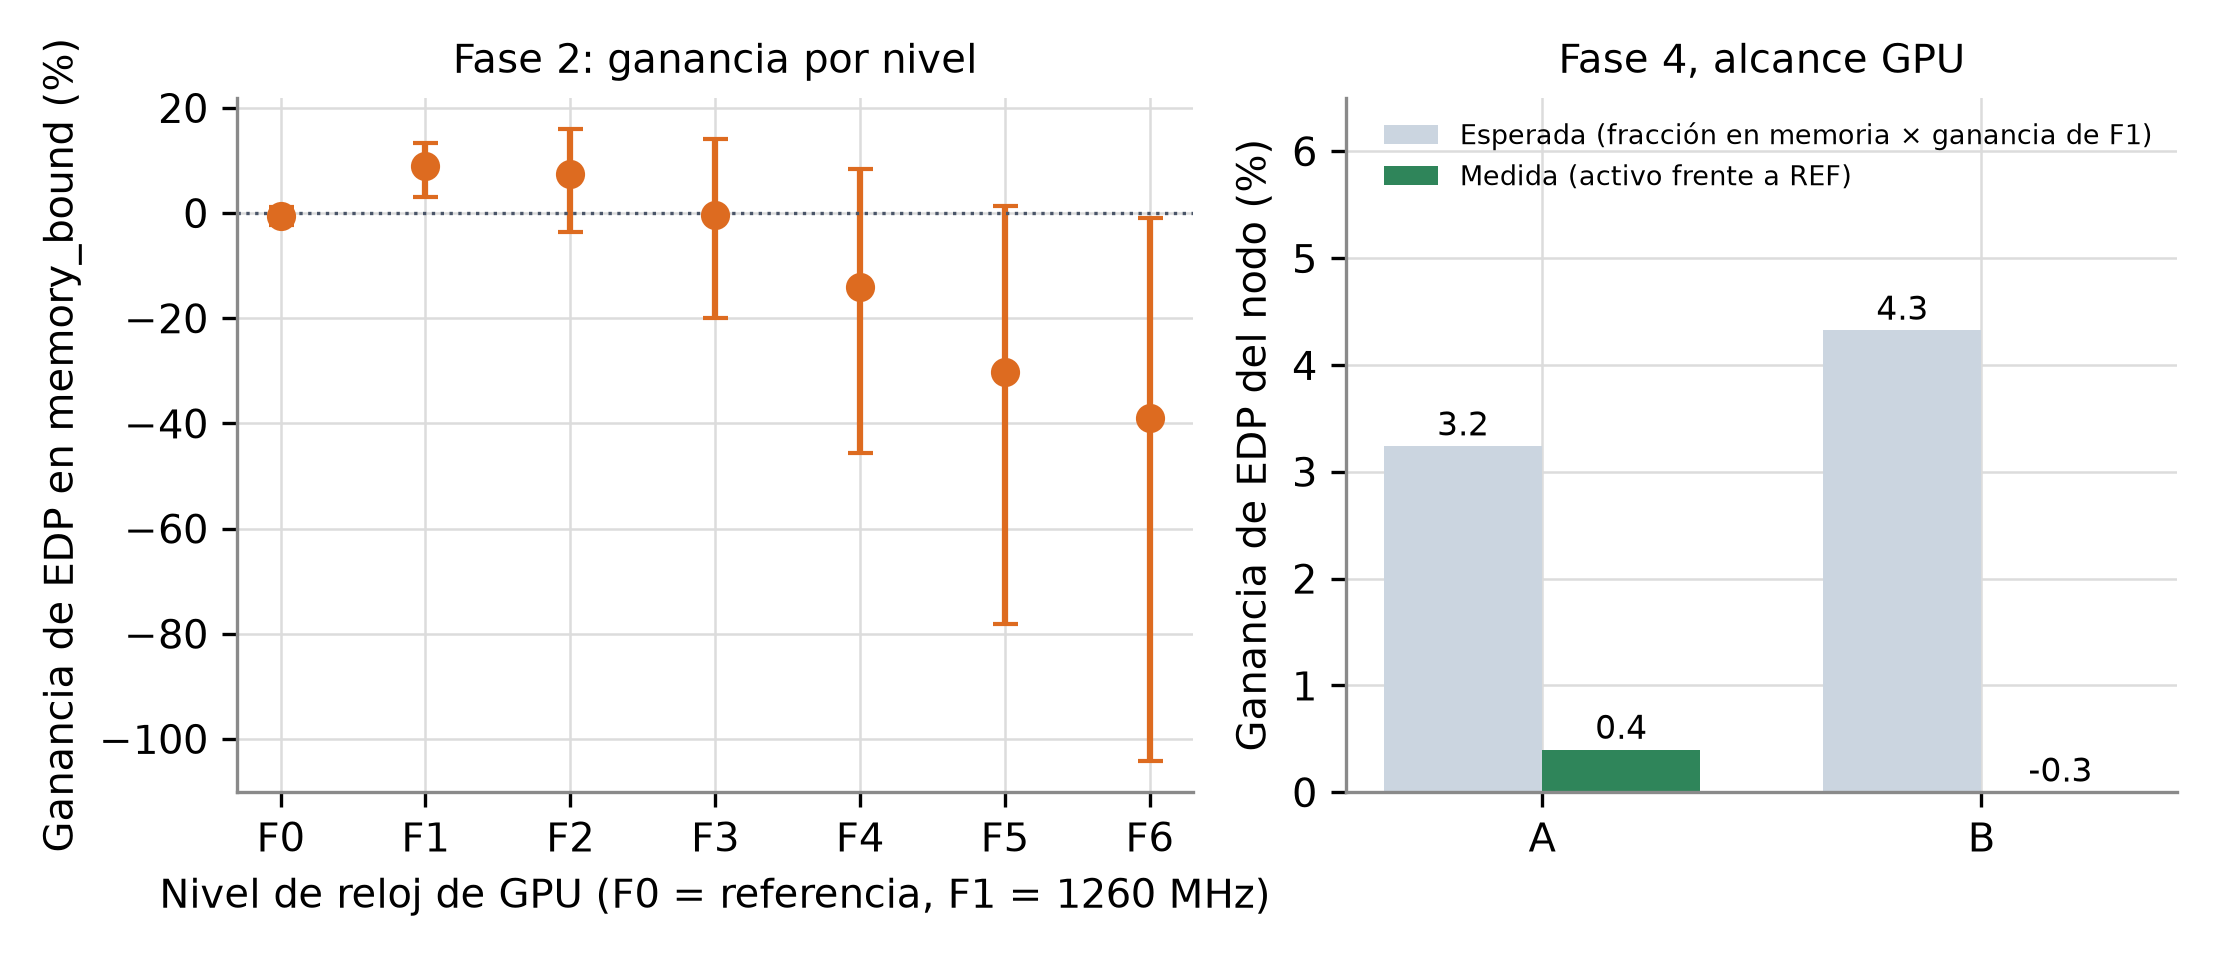
\includegraphics[width=\textwidth]{figuras/fig_fase4_gpu_potencial_20260924.png}
    \caption{Izquierda: ganancia de EDP por nivel de reloj de GPU en fases \textit{memory\_bound} (Fase 2, IC95 sobre familias). Derecha: ganancia esperada (fracción de tiempo en memoria por la ganancia de F1) frente a la medida con el agente activo en el alcance GPU.}
    \label{fig:fase4-gpu}
\end{figure}

En A, el agente clasificó las dos fases de \textit{triad} y aplicó F1 en ambas, y aun así la ganancia medida queda por debajo de la esperada: con tres repeticiones no puede separarse de cero y su causa no está aislada. En B, las fases de BabelStream, de 8~s, se resolvieron con una sola decisión cada una y en las celdas revisadas esa decisión fue una abstención, así que el reloj no se bajó. La ganancia posible de la GPU depende entonces de dos condiciones: que la aplicación pase una parte apreciable del tiempo en fases largas \textit{memory\_bound}, y que el agente no se abstenga en ellas. El escenario E de la sección \ref{sec:resultados-fase4-E} evalúa ambas.

\subsection{Escenario C: agente de CPU con un hilo de inferencia}
\label{sec:resultados-fase4-C}

Este escenario repite el alcance de CPU y el conjunto con el agente en su configuración final (un hilo de inferencia, sección \ref{sec:resultados-fase4-costo}), con tres repeticiones por brazo (Tabla \ref{tab:fase4-C} y Figura \ref{fig:fase4-C}). El costo de mantener el agente pasó a ser pequeño: el brazo sombra queda entre 1.036 y 1.094 del EDP de REF, con un exceso de tiempo de 0.4 a 1.4\% y un exceso de energía de CPU de 5 a 9\%. El brazo activo queda entre 1.05 y 1.16 y no mejora sobre sombra: el cociente activo/sombra es 1.06, 1.00, 1.02 y 1.01. En CPU con kernels vistos, bajar a F1 en memoria (1.161) es peor que mantener F0 (1.096). Quitar el piso de coordinación en el alcance conjunto empeora el EDP entre 0.8 y 1.3 puntos, de modo que el piso tiene un efecto pequeño pero favorable. La clasificación mantiene su exactitud con el agente corregido: 97.6\% en A y 99.9\% en B en CPU, sin errores en las decisiones de GPU (Tabla \ref{tab:fase4-clasificacion-CE}).

\begin{figure}[H]
    \centering
    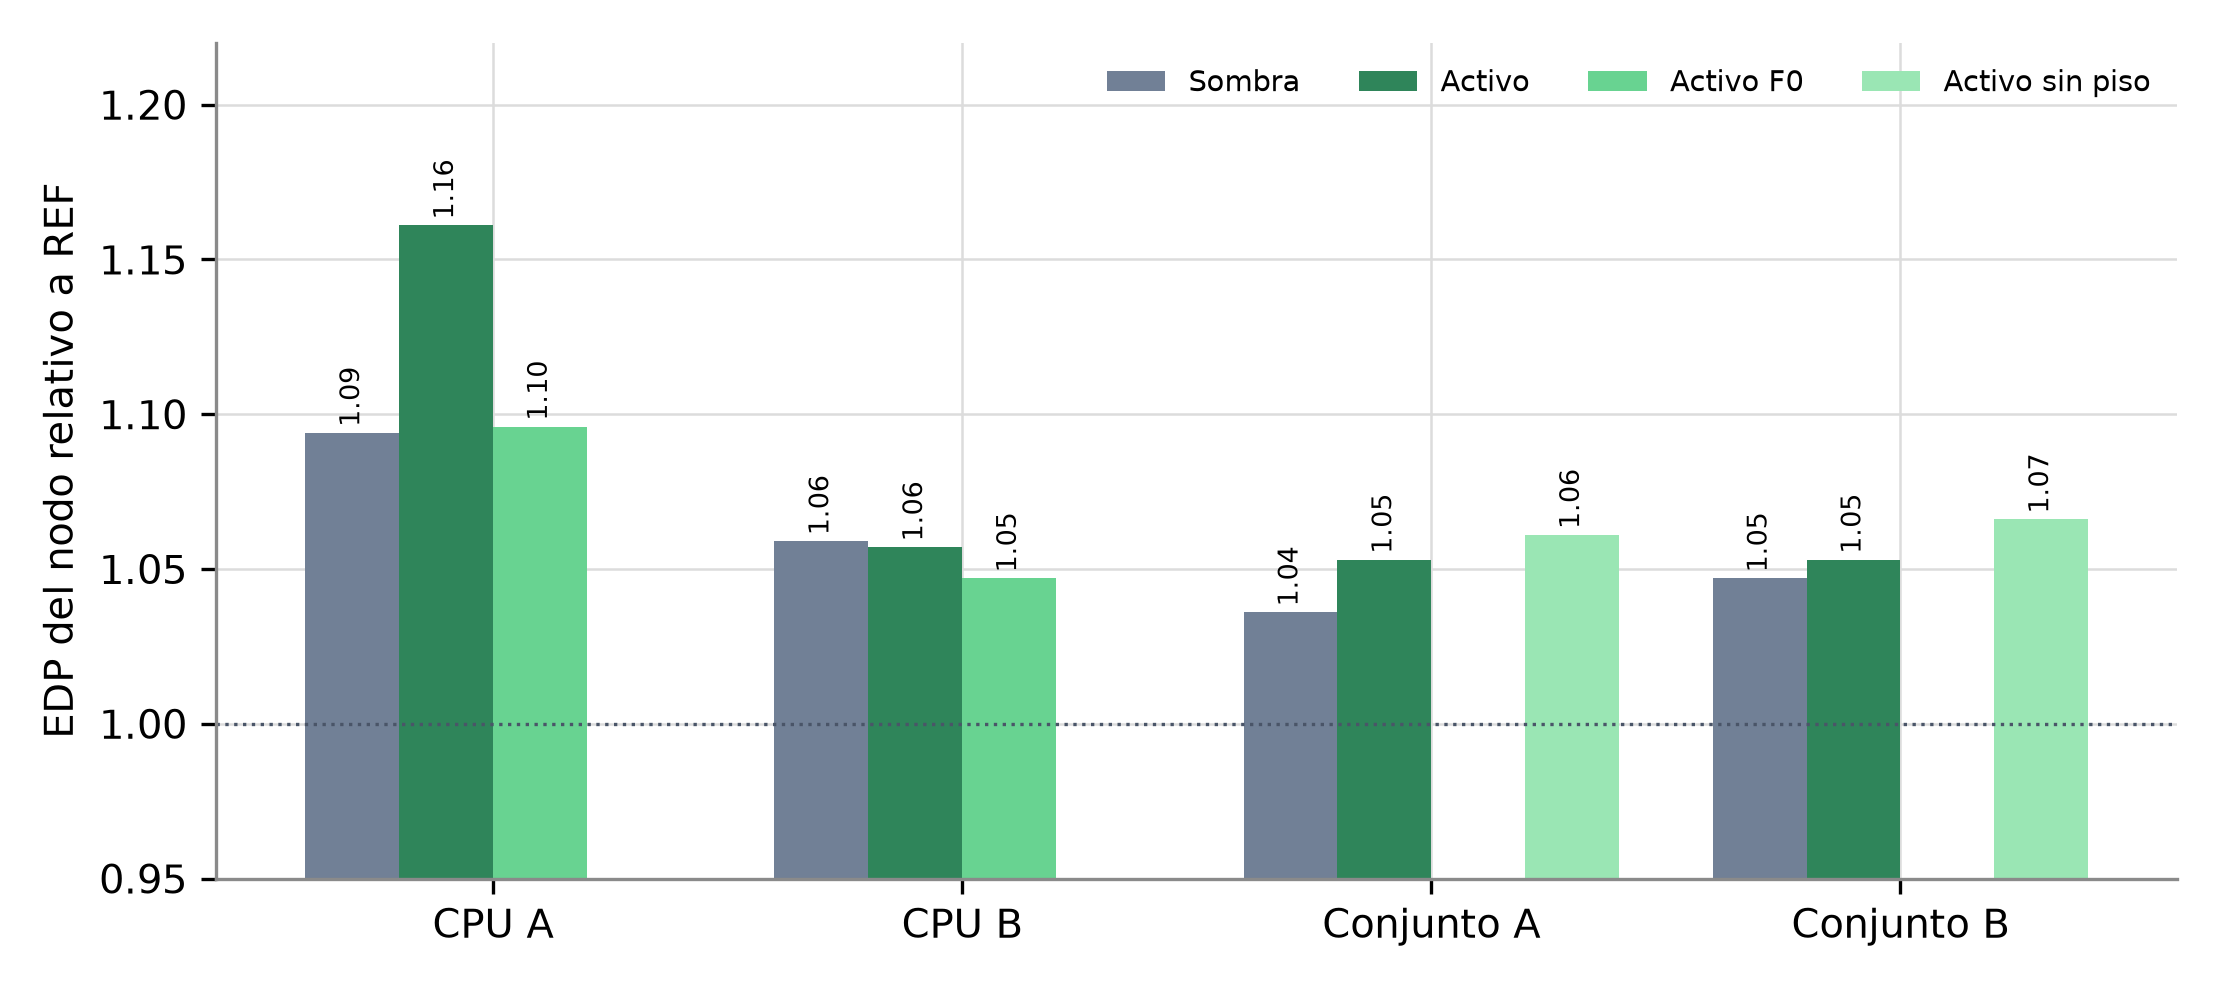
\includegraphics[width=\textwidth]{figuras/fig_fase4_C_edp_20260924.png}
    \caption{EDP del nodo relativo a REF en el escenario C, por alcance, aplicación y brazo. La línea punteada marca la paridad con REF.}
    \label{fig:fase4-C}
\end{figure}



\subsection{Referencia sin turbo}
\label{sec:resultados-fase4-noturbo}

REF sin turbo produjo razones medianas de EDP de 0.988 a 1.006 frente a REF en las seis combinaciones compuestas medidas (Tabla \ref{tab:fase4-noturbo}). En estas cargas el turbo no elevó el reloj sobre el límite de 3.2~GHz; por ello, las conclusiones CPU no dependen de esa línea base. La comparación no se extiende a LAMMPS ni CloverLeaf, ni sustituye un brazo de GPU con F1 fijo.



\subsection{Escenario E: GPU dominada por fases de memoria}
\label{sec:resultados-fase4-E}

El escenario E mide la política de GPU en las condiciones en que la Fase 2 predice ganancia: aplicaciones cuyo tiempo se reparte sobre todo en fases \textit{memory\_bound} largas. Es un escenario de aplicabilidad y no representa cualquier carga. Se definió antes de ejecutarse con un criterio de selección explícito: familias \textit{memory\_bound} cuya ganancia de EDP con F1 en la Fase 2 fue de al menos 10\%, más una variante con familias no vistas en el entrenamiento. La duración de las fases sale de una medición previa: el agente de GPU decide una vez por fase y la primera decisión llega entre 13 y 16~s después de su inicio, de modo que fases de 18~s pasan solo la mitad de su tiempo en F1 y fases de 45 a 60~s pasan más del 70\%.

La Tabla \ref{tab:fase4-E-composicion} resume las dos aplicaciones declaradas antes de medir. En B, \textit{myocyte} recibe una etiqueta de memoria por kernel pero casi no ocupa la GPU; solo el 42\% del ciclo corresponde a memoria con actividad GPU. Esta diferencia entre etiqueta y oportunidad de actuación condiciona la interpretación del resultado.

\begin{table}[H]
\centering
\caption{Composición del escenario E. Duraciones aproximadas por fase medidas antes de la matriz.}
\label{tab:fase4-E-composicion}
\small
\setlength{\tabcolsep}{3pt}
\begin{tabular}{@{}p{2.0cm}p{7.2cm}p{3.8cm}@{}}
\toprule
\textbf{Aplicación} & \textbf{Fases} & \textbf{Tiempo etiquetado memoria} \\
\midrule
A (vistas) & Stencil (58--60~s), SpMV (46~s), AXPY (47--48~s); DGEMM cómputo (31~s) & 84\% del ciclo \\
B (inéditas) & BabelStream (36~s), Myocyte (40--41~s); LavaMD cómputo (9~s) & 89\% etiquetado; 42\% con actividad GPU de memoria \\
\bottomrule
\end{tabular}
\end{table}

\paragraph{Medición exploratoria en familias vistas (A).} La medición exploratoria ejecutó tres repeticiones con REF, sombra y agente activo. El agente activo redujo la energía de GPU en 7.1\% (0.929 de REF), mantuvo la duración (1.000) y redujo el EDP del nodo a 0.975 y el EDP de GPU sola a 0.928 (Tabla \ref{tab:fase4-E} y Figura \ref{fig:fase4-E}). Sombra quedó en 0.995 del EDP de REF, lo que localiza la mayor parte del ahorro en la actuación F1. El agente clasificó y aplicó F1 en las fases de memoria previstas. La confirmación prospectiva de cinco bloques se reporta por separado a continuación.

El ahorro del nodo es modesto porque la CPU consume el 64\% de la energía en esta aplicación y no se modifica. Con el agente de CPU en observación, el EDP del nodo vuelve a 1.003, porque su costo (2.9\% más de energía de CPU y 1.0\% más de tiempo) iguala el ahorro de GPU. La configuración que mejora es, por tanto, la de un agente de GPU sin agente de CPU, coherente con la política de CPU de no actuar.

\paragraph{Confirmación prospectiva de E-A.} La mejora frente a REF se repitió en un confirmatorio declarado antes de medir, con cinco bloques aleatorizados y cinco repeticiones válidas por brazo. El brazo activo redujo la energía de GPU a 0.9282 de REF, mantuvo la duración en 0.9990 y dejó el EDP del nodo en 0.9716, equivalente a una reducción de 2.84\%. El brazo sombra quedó en 0.9935, por lo que el efecto no se explica por el costo de observación. Las cinco diferencias activo--REF fueron favorables; con bloques como unidad, la prueba exacta bilateral tiene $p=0.0625$, el mínimo posible para este diseño. El brazo F1 fijo no produjo celdas válidas, porque el reloj observado bajo carga quedó fuera del intervalo de 1230--1290~MHz exigido por el protocolo. Por ello, el confirmatorio reproduce la mejora frente a REF, pero no permite establecer la ventaja del cambio por fase frente a mantener F1 durante toda la aplicación.

\paragraph{Premedición de F1 fijo.} Antes del confirmatorio se ejecutó la medición diagnóstica F, con cinco repeticiones de REF y de una solicitud de F1 en DGEMM de CUTLASS, Conv2D y LavaMD. No se integra con E-A ni se usa para estimar el efecto del agente. En Conv2D y LavaMD, el EDP de GPU sola fue 0.894 y 0.960 de REF, respectivamente, pero el EDP del nodo fue 1.017 y 1.024 por el aumento del tiempo. En DGEMM, el reloj observado con F1 solicitado fue de 1140 a 1155~MHz, indistinguible de REF, por lo que esa comparación no valida una actuación a 1260~MHz. Este antecedente motivó el criterio de reloj bajo carga que después invalidó el brazo fijo del confirmatorio E-A.

\paragraph{Familias inéditas (B).} La mediana quedó cerca de paridad (EDP de nodo 1.014 y energía GPU 1.003 de REF). BabelStream recibió una decisión de memoria en una de tres repeticiones y allí ahorró 12\% de energía GPU y 5\% de EDP del nodo; en las otras dos se abstuvo. \textit{Myocyte} no superó sostenidamente el umbral de actividad GPU y no recibió decisión. Una demora aislada de esa fase ocurrió sin cambio de reloj atribuible al agente. El límite observado es la cobertura de decisión sobre familias inéditas, no un empeoramiento sistemático por F1.

\begin{figure}[H]
    \centering
    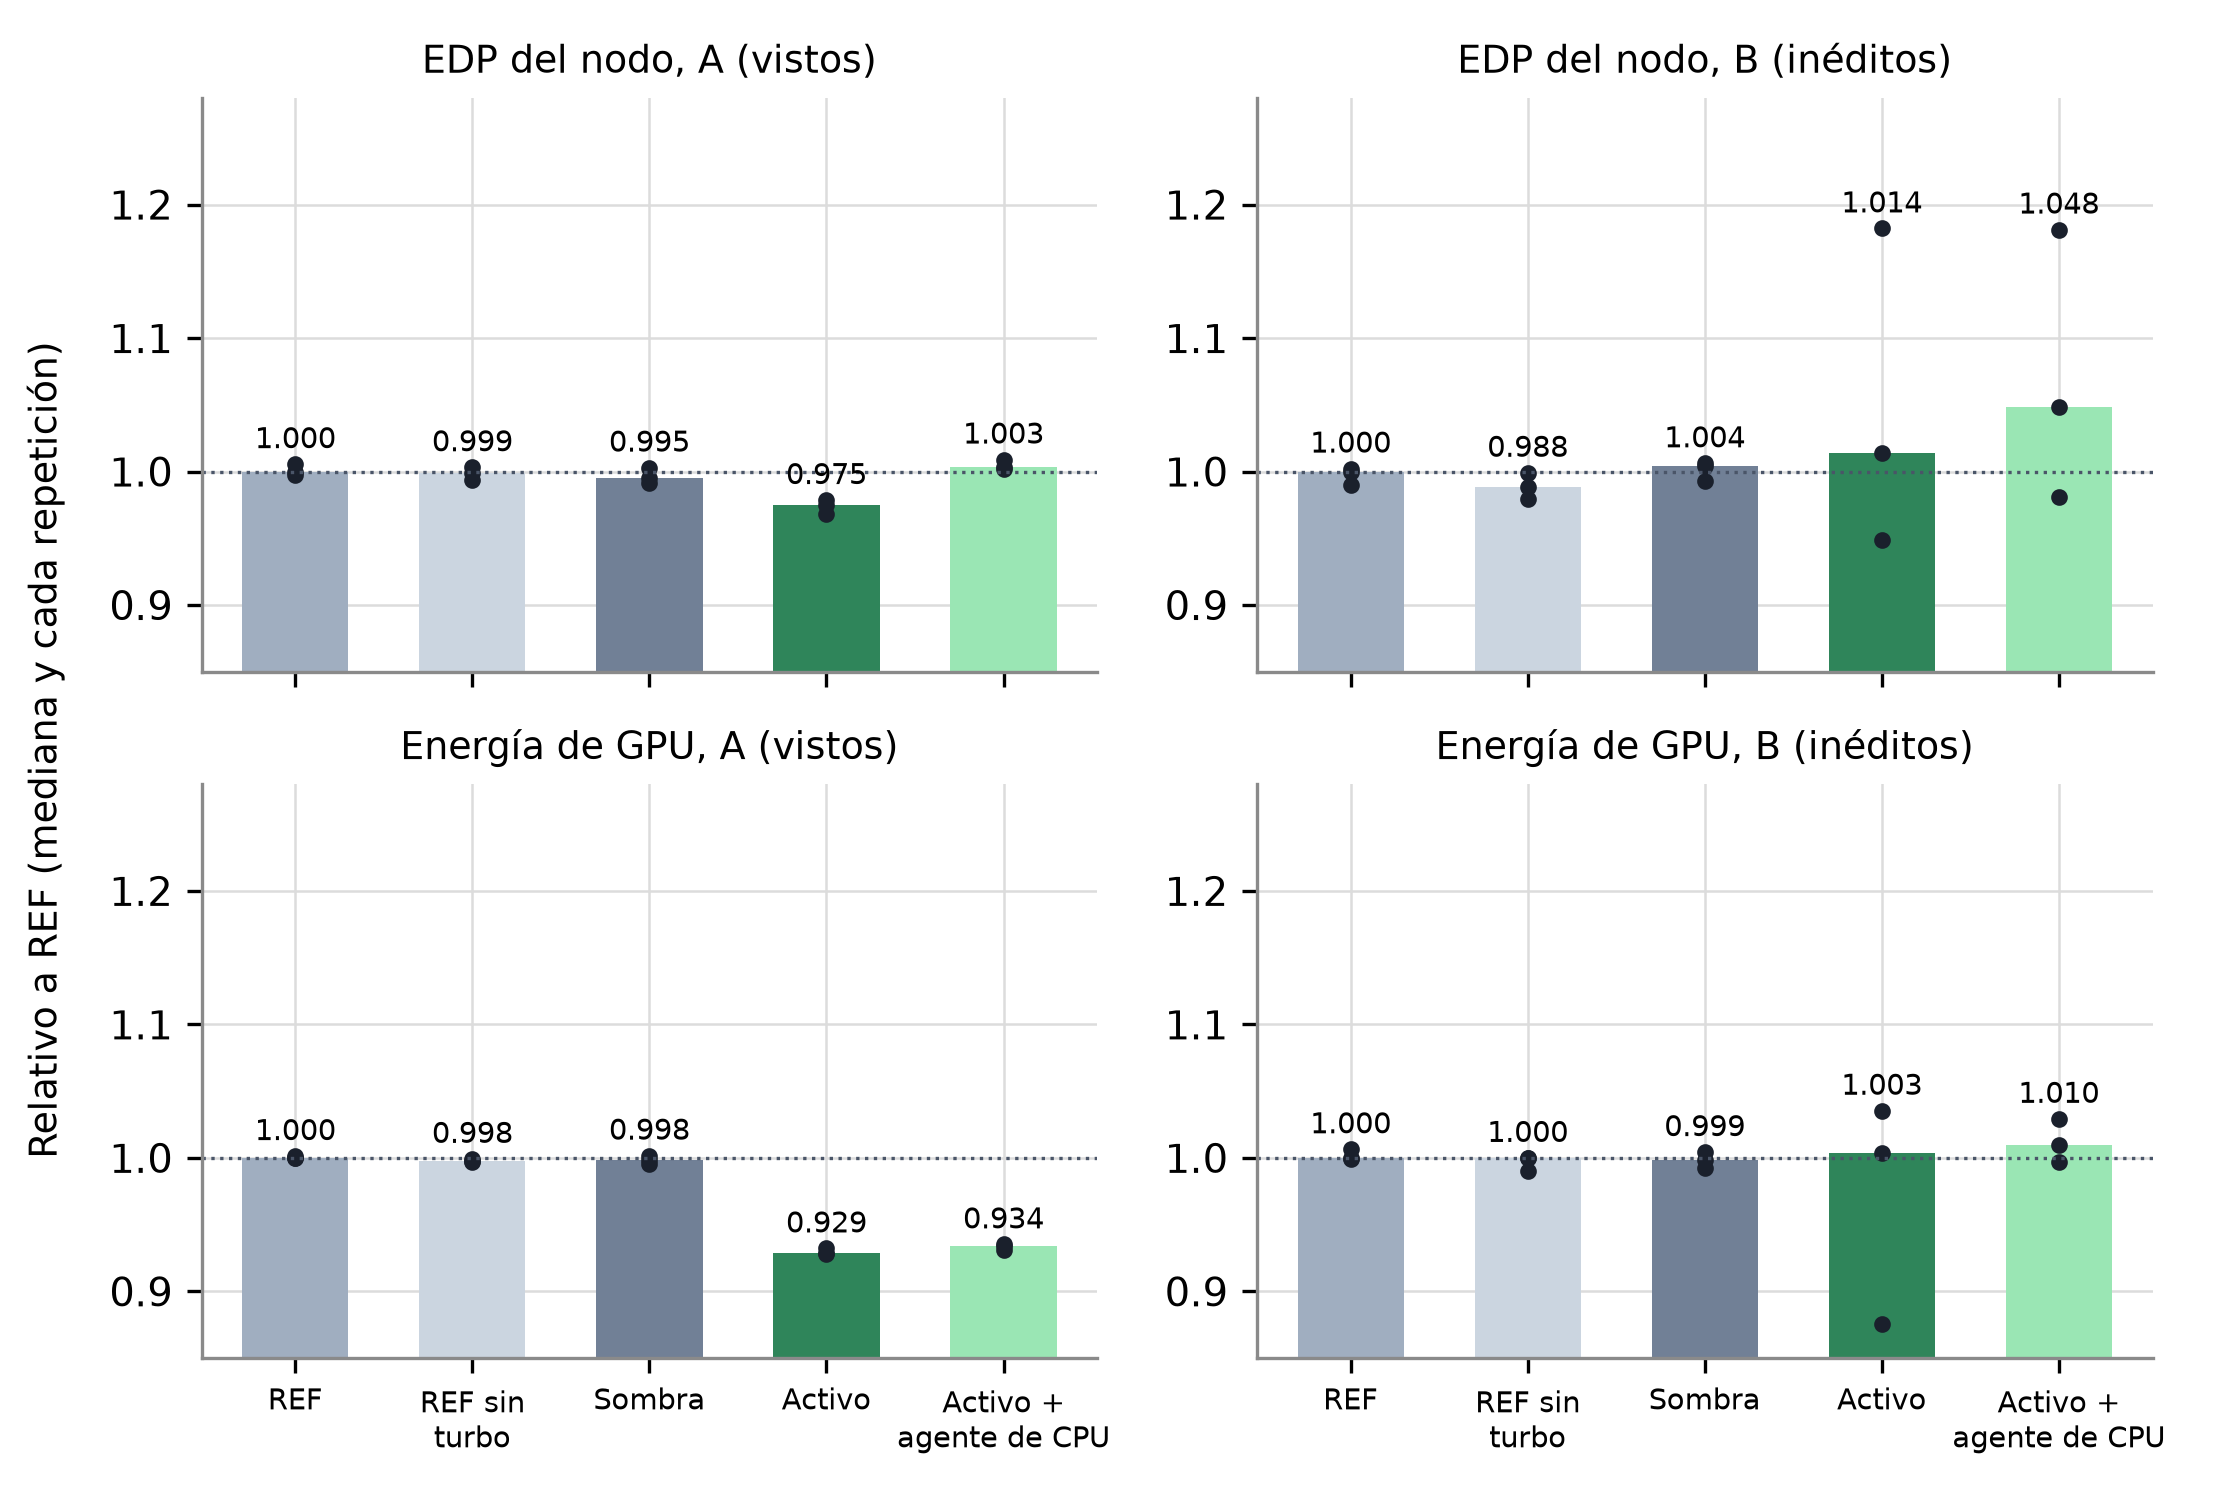
\includegraphics[width=\textwidth]{figuras/fig_fase4_E_20260924.png}
    \caption{Escenario E. EDP del nodo (arriba) y energía de GPU (abajo) relativos a REF, con la mediana (barra) y cada repetición (punto), para las aplicaciones de familias vistas (A) e inéditas (B).}
    \label{fig:fase4-E}
\end{figure}





\subsection{Escenario D: LAMMPS como aplicación de terceros}
\label{sec:resultados-fase4-D}

El escenario D evalúa LAMMPS 2023 con el paquete GPU del clúster, sin imponer fronteras de fase al programa. Se ejecutaron tres bloques de las entradas \texttt{chain}, \texttt{eam}, \texttt{lj} y \texttt{rhodo}, con REF, sombra, agente de GPU activo y una variante que mantiene el agente de CPU en observación. Todas las 48 celdas terminaron con código de aplicación y de daemon válido, y restauraron el estado de frecuencia. La Figura \ref{fig:fase4-D} y la Tabla \ref{tab:fase4-D} muestran que el brazo activo de GPU queda entre 0.998 y 1.008 de REF en EDP, según la entrada. No se observa una mejora persistente y la variante con el agente de CPU en observación incrementa el EDP entre 3.0 y 4.3\%. En \texttt{chain} y \texttt{rhodo} el agente no emitió decisiones y en \texttt{lj} y \texttt{eam} solo emitió \textit{compute\_bound}, por lo que no aplicó F1. Este resultado extiende la evaluación a una aplicación externa, pero no mide el efecto de la política GPU sobre una fase actuada.

\begin{figure}[H]
    \centering
    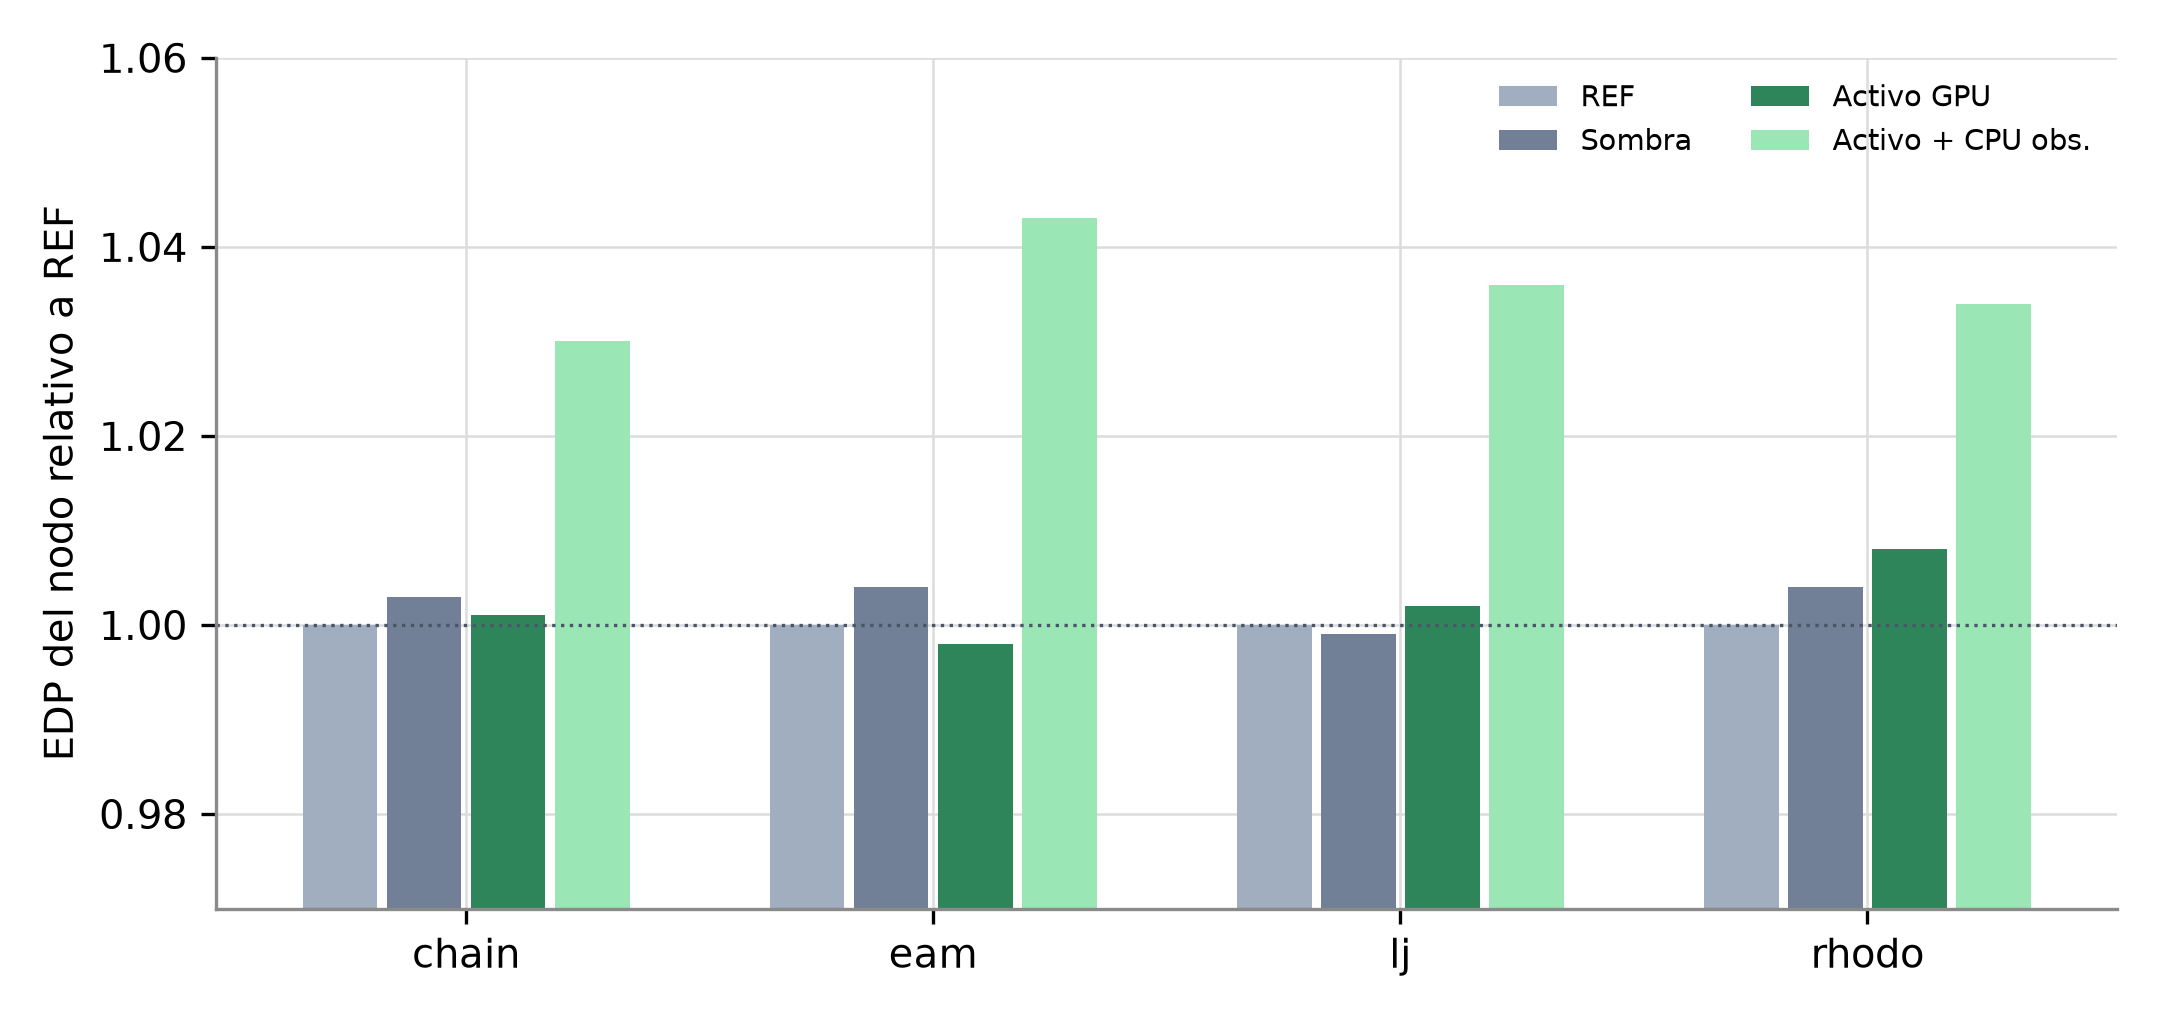
\includegraphics[width=0.88\textwidth]{figuras/fig_fase4_D_20260924.png}
    \caption{EDP mediano de LAMMPS por entrada y brazo, relativo a REF. Fuente: elaboración propia.}
    \label{fig:fase4-D}
\end{figure}



\subsection{CloverLeaf CUDA Fortran como aplicación continua}
\label{sec:resultados-fase4-cloverleaf}

CloverLeaf CUDA Fortran se evaluó como una aplicación continua de dinámica de fluidos, sin fronteras de fase impuestas al programa. El confirmatorio ejecutó cinco bloques aleatorizados con REF, sombra y activo. Las quince corridas terminaron con código de aplicación válido, restauración correcta del reloj y solución numérica reproducible; la energía cinética final fue idéntica dentro de la tolerancia relativa de $10^{-8}$. En cada corrida activa el agente emitió una decisión \textit{memory\_bound} con confianza 1.00 tras aproximadamente 3~s y solicitó 1260~MHz. Tras esa decisión, las 433 o 434 muestras NVML bajo carga de cada bloque permanecieron en 1260~MHz. CloverLeaf no aporta una etiqueta Roofline independiente por fase, de modo que este experimento verifica la actuación y su efecto energético, pero no puntúa la exactitud de esa decisión. La Tabla \ref{tab:fase4-cloverleaf} resume las medianas y las razones frente a REF.

El brazo activo mantuvo la duración en 1.0015 de REF, redujo la energía de GPU a 0.9393 y dejó el EDP del nodo en 0.9625, una reducción de 3.75\%. El brazo sombra quedó en 0.9958 de EDP, por lo que no se observa un costo apreciable de mantener el agente sin actuar. Las cinco diferencias de EDP activo--REF fueron favorables; la prueba exacta bilateral por bloques da $p=0.0625$, que no alcanza el umbral de 0.05. La Figura \ref{fig:fase4-cloverleaf-edp} muestra las cinco observaciones emparejadas por bloque y la Figura \ref{fig:fase4-cloverleaf-energia} descompone el resultado entre CPU y GPU. En este caso, la actuación reduce la energía del dispositivo sin modificar de forma apreciable el tiempo de ejecución.

\begin{figure}[H]
    \centering
    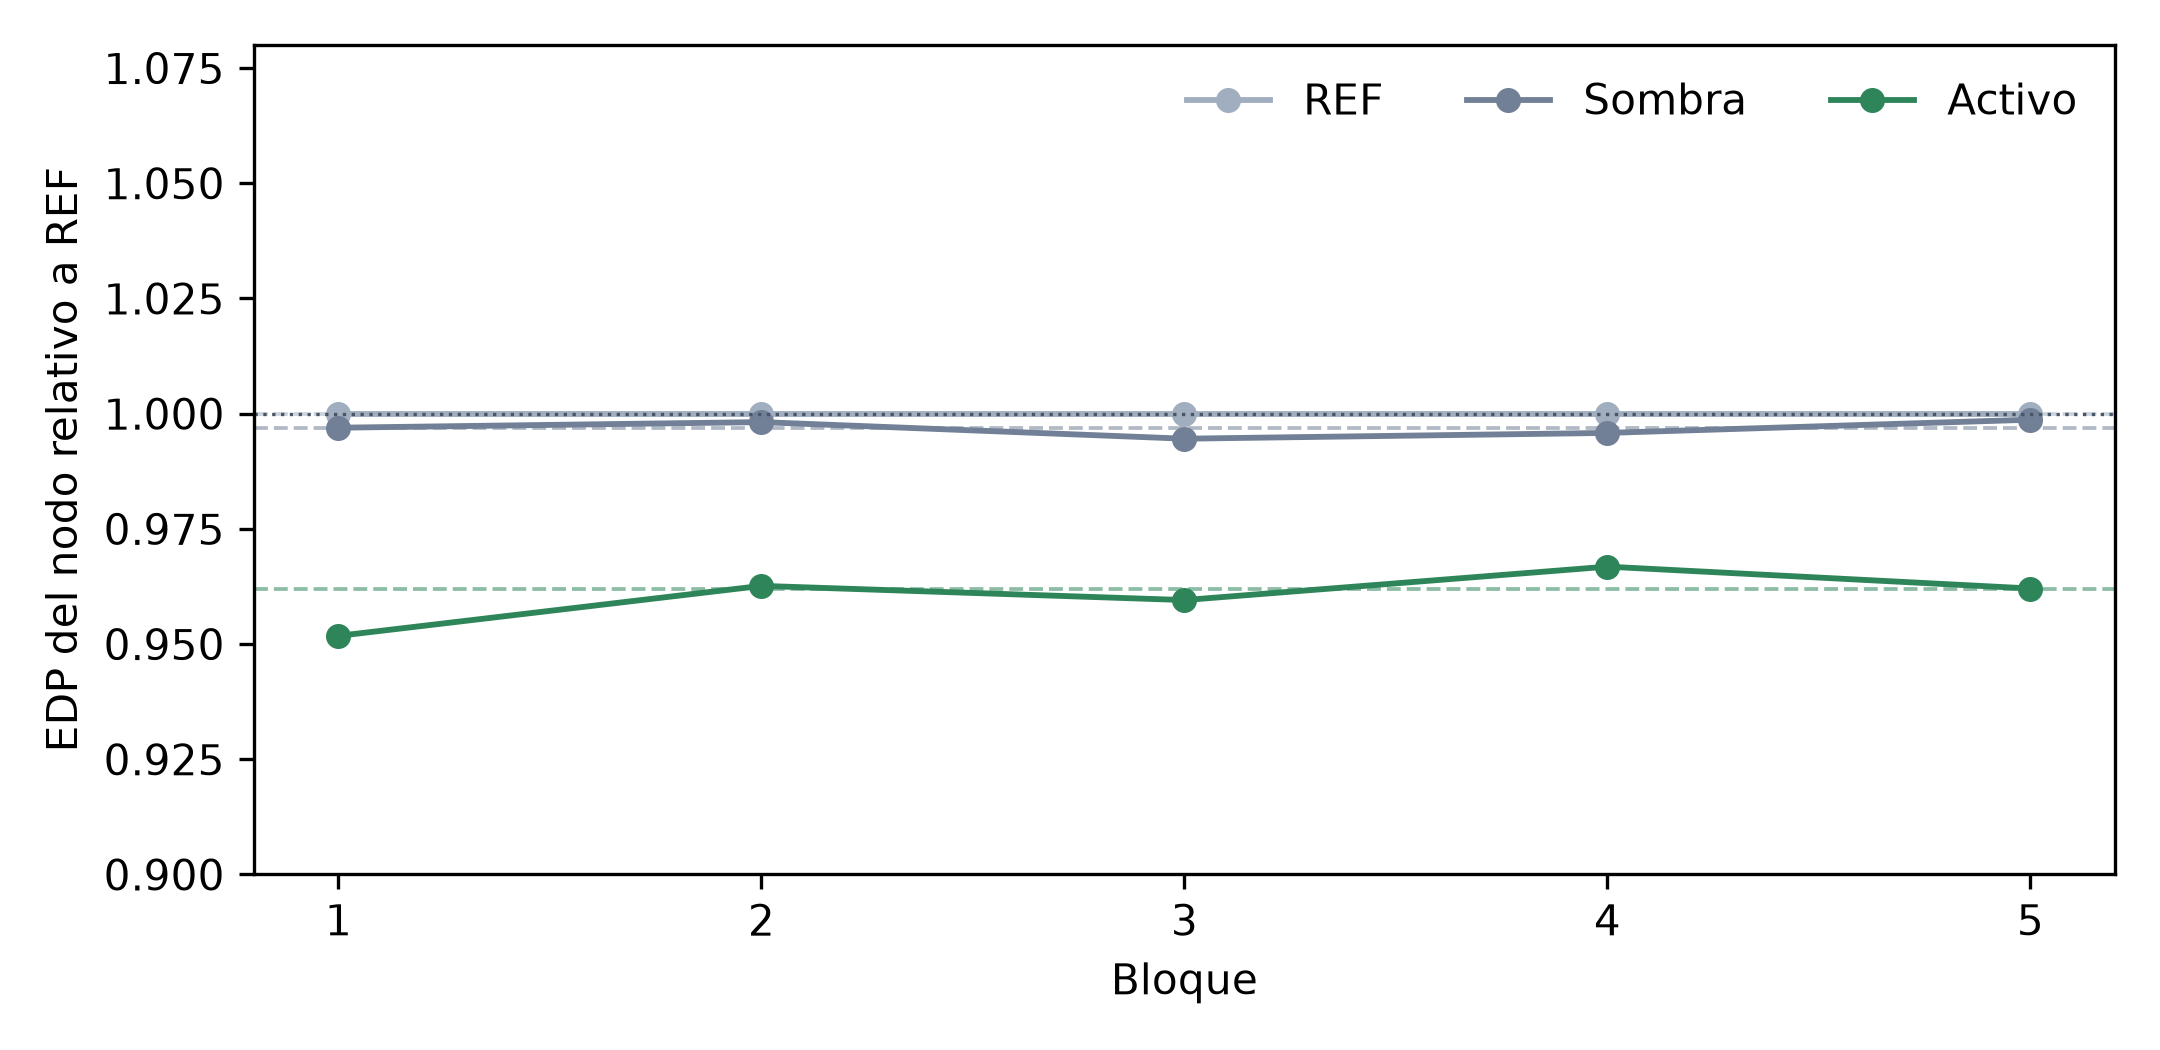
\includegraphics[width=0.90\textwidth]{figuras/fig_fase4_cloverleaf_edp_20260924.png}
    \caption[EDP de CloverLeaf por bloque y brazo]{EDP del nodo de CloverLeaf relativo a REF en cada bloque. Las líneas discontinuas indican la mediana de cada brazo y la línea punteada marca la paridad con REF. Fuente: elaboración propia a partir de cinco bloques del nodo \texttt{paccaA100}.}
    \label{fig:fase4-cloverleaf-edp}
\end{figure}

\begin{figure}[H]
    \centering
    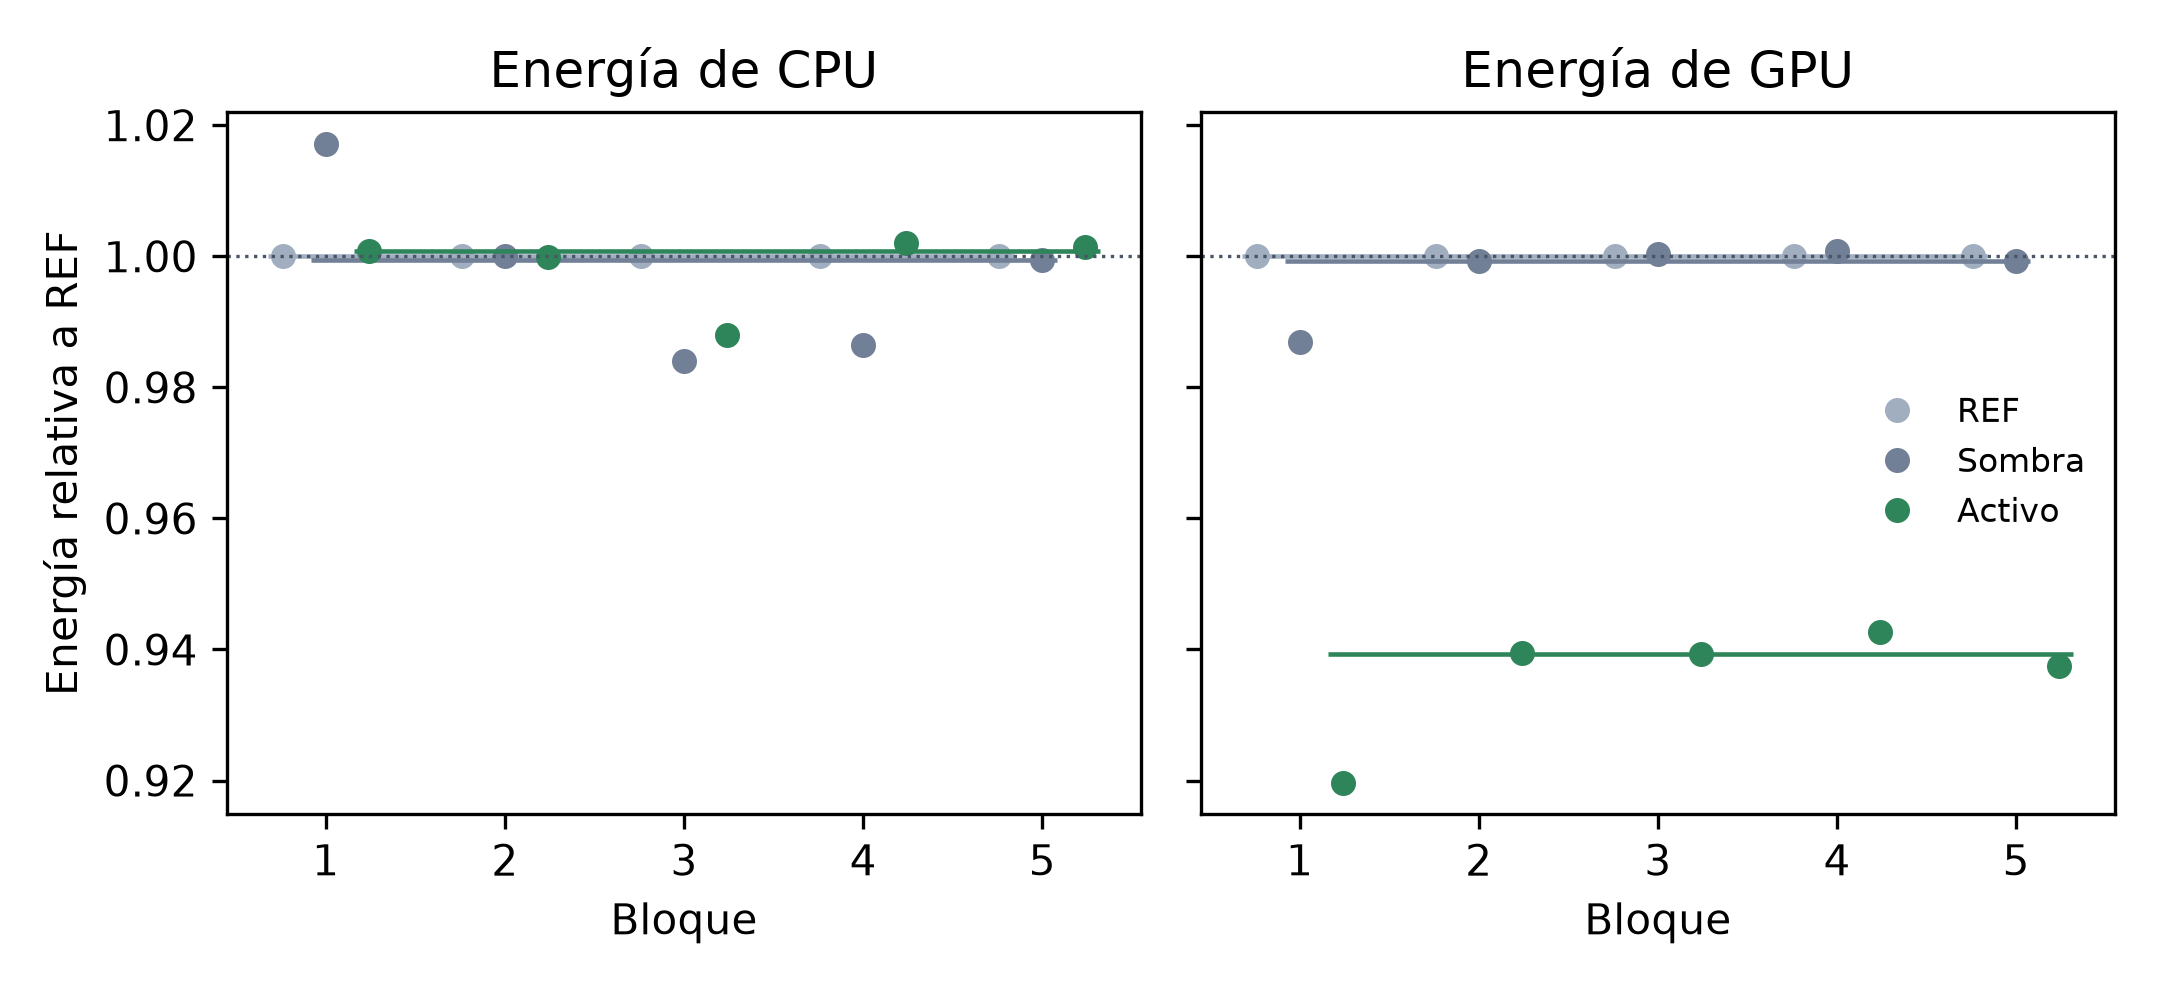
\includegraphics[width=0.90\textwidth]{figuras/fig_fase4_cloverleaf_energia_20260924.png}
    \caption[Descomposición de energía de CloverLeaf]{Energía de CPU y GPU de CloverLeaf relativa a REF en los cinco bloques. Los puntos representan bloques individuales y las líneas horizontales, las medianas por brazo. Fuente: elaboración propia.}
    \label{fig:fase4-cloverleaf-energia}
\end{figure}





\begin{table}[H]
\centering
\caption{Resultados del confirmatorio de CloverLeaf CUDA Fortran. Duración y energías son medianas de cinco bloques; las razones se calculan frente a REF.}
\label{tab:fase4-cloverleaf}
\small
\begin{adjustbox}{max width=\textwidth}
\begin{tabular}{@{}lrrrrrr@{}}
\toprule
\textbf{Brazo} & \textbf{$n$} & \textbf{$T$ (s)} & \textbf{$E_{\mathrm{CPU}}$ (J)} & \textbf{$E_{\mathrm{GPU}}$ (J)} & \textbf{EDP/REF} & \textbf{$E_{\mathrm{GPU}}$/REF} \\
\midrule
REF & 5 & 112.032 & 16939.3 & 27729.5 & 1.0000 & 1.0000 \\
Sombra & 5 & 111.975 & 16923.4 & 27733.6 & 0.9958 & 1.0001 \\
Activo & 5 & 112.201 & 16957.7 & 26044.9 & 0.9625 & 0.9393 \\
\bottomrule
\end{tabular}

\end{adjustbox}
\end{table}

\subsection{Balance de la Fase 4}
\label{sec:resultados-fase4-balance}

La Tabla \ref{tab:fase4-balance} reúne la respuesta a cada pregunta de la Fase 4 y distingue los resultados favorables, neutros y no demostrados.

\begin{table}[H]
\centering
\caption{Balance de la Fase 4. El desglose por pregunta se conserva en la Tabla \ref{tab:fase4-balance-detalle} del Anexo \ref{anexo:resultados-complementarios}.}
\label{tab:fase4-balance}
\small
\begin{tabular}{@{}p{3.5cm}p{9.8cm}@{}}
\toprule
\textbf{Pregunta} & \textbf{Resultado} \\
\midrule
Clasificación & Alta en aplicaciones con verdad conocida; la GPU se abstiene con frecuencia ante familias inéditas \\
Costo de observación & GPU sin costo medible; CPU con un hilo añade 5 a 9\% de energía \\
Actuación CPU & Sin mejora de EDP frente a REF ni frente a sombra \\
Actuación GPU & E-A: $-2.84\%$ de EDP del nodo; CloverLeaf: $-3.75\%$; LAMMPS: paridad \\
F1 fijo & La comparación directa quedó inválida por reloj no sostenido bajo carga \\
\bottomrule
\end{tabular}
\end{table}
